% !Mode:: "TeX:UTF-8"
\documentclass[doctor]{bnuthesis}
% \documentclass[%
%   bachelor|master|doctor, % 学士、硕士、博士 
%   xetex|pdftex|dvips|dvipdfm, % 可选编译方式
%   openany|operight,  % 连续页面,或者右侧打开
%   secret,  % 是否涉密
%   arialtoc,arialtitle]{bnuthesis}

% 所有其它可能用到的包都统一放在这里,可以根据实际需要添加或者删除。
\usepackage{bnutils}

% 这三条命令使用自动调整宽度的表格
% https://zhuanlan.zhihu.com/p/542672514
\usepackage{tabularx} % for 'tabularx' env. and 'X' col. type
\usepackage{ragged2e} % for \RaggedRight macro
\usepackage{booktabs} % for \toprule, \midrule etc macros
%% create a derivative column type called 'L':
\newcolumntype{L}{>{\RaggedRight\hangafter=1\hangindent=0em}X}

% 你可以在这里修改配置文件中的定义,导言区可以使用中文。
% \def\myname{薛瑞尼}


\begin{document}
% 定义所有的eps文件在figures子目录下
\graphicspath{{img/}}

%%% 封面部分
\frontmatter
% !Mode:: "TeX:UTF-8"

\ctitle{流域治理视角下黄河人-水关系演变过程及驱动机制}
\etitle{Co-evolution of human-water interactions from a governing perspective in the Yellow River Basin, China: processes and mechanism}


\makeatother

% 学士学位封面
% \cbuyuanxi{天文系} % 部院系
% \czhuanye{天文学} % 专业
% \cxuehao{201511160109} % 学号
% \cxueshengxingming{某某某} % 学生姓名
% \czhidaojiaoshi{某某} % 指导教师
% \czhidaojiaoshizhicheng{教授} % 指导教师职称
% \czhidaojiaoshidanwei{北京师范大学天文系} % 指导教师单位

% 博士(硕士)学位封面
\czuozhe{宋爽} % 作者
\cdaoshi{傅伯杰\ 教授} % 导师
\cxibienianji{地理学部2018级} % 系别年级
\cxuehao{201831051016} % 学号
\cxuekezhuanye{自然地理} % 学科专业
\cwanchengriqi{2023年4月} % 完成日期


\begin{cabstract}
% 论文的摘要是对论文研究内容和成果的高度概括。摘要应对论文所研究的问题及其研究目的进行描述,对研究方法和过程进行简单介绍,对研究成果和所得结论进行概括。摘要应具有独立性和自明性,其内容应包含与论文全文同等量的主要信息。使读者即使不阅读全文,通过摘要就能了解论文的总体内容和主要成果。

% 论文摘要的书写应力求精确、简明。切忌写成对论文书写内容进行提要的形式,尤其要避免“第 1 章……;第 2 章……;……”这种或类似的陈述方式。

% 本文介绍北京师范大学论文模板 BNUThesis 的使用方法。本模板是在清华大学学位论文模板 THUThesis 的基础上修改而来,以及BNU硕博士模板BNUThesis上修改完成。完全参照《毕业论文写作规范(修订)》(师教文[2007]186 号)、北京师范大学图书馆Word版学士模板、北京师范大学信息科学与技术学院Word版写作模板的格式要求制作而成。

大河流域是人类起源和发展的中心,随着人类活动改变了流域的自然和社会水循环过程,许多大河流域出现了不可持续的发展态势。
治理黄河是中华民族的千年夙愿,重塑黄河人水关系、实现黄河流域生态保护和高质量发展也是国家的重大战略。
因此,研究黄河流域人水关系演变规律、揭示演变机制,可为黄河流域治理提供理论基础和科学依据。
本研究结合水文气象观测、社会经济统计、历史数据重建和遥感反演等多源数据,借助统计分析、因果推断、与多主体建模等手段,发展了流域人水关系演变的识别与分析框架及机制分析方法,在历史时期和现代治黄时期定量划分黄河流域人水关系演变的主要阶段与过程、识别了推动人水关系变化的关键机制,主要研究结论如下:

(1)历史时期黄河流域存水沙变化的在两个湿润气候驱动期($900AD\sim1100AD$和$1700AD\sim1900AD$)和两个人类活动驱动期($1350AD \sim 1650AD$ 和 $1900AD$迄今)。其中第一个气候驱动期位于“中世纪暖期”(约$900AD \sim 1100AD$),此时黄河的水沙变化变化仍由气候因素主导。随后中游黄土高原地区发生农田与人口的快速扩张,不断增加的人为压力与另一次潮湿气候共同推动水沙特征在$1700AD \sim 1900AD$越过变化的临界点。上述结果表明人类活动带来的影响最早追溯至$1350AD$才开始取代周期变化的气候,逐步成为历史时期主导黄河流域人-水关系的主要因素。

(2)本研究使用综合水治理指数(IWGI)将当代治黄时期的流域水治理演变过程划分为三个阶段,并依据其各自特点命名为:集中供水时期($1965 \sim 1978$年)、治理转变时期($1979 \sim 2001$年)、以及适应增强时期($2002 \sim 2013$年)。灌区扩张和水库修建的放缓,是黄河从集中供水时期向治理转变时期过渡的主要特征。在治理转变时期流域的非工程治理措施迅速增加,过渡至适应增强时期后保持稳定,并着重提升用水效率。经讨论,上述治理模式转变可能在全世界流域系统中普遍存在,而本研究的分析指出水资源供给趋近极限可能是触发转变的关键。

(3)在上述治理转变期,$1987$年提出的黄河水资源配额制度及其在$1998$年的改革,是对流域影响深远的典型非工程治理政策。本研究指出这两次制度变化以不同的方式重塑了黄河流域的社会-生态系统结构,因而较政策初衷而言产生了不同的治理效果。其中,$1987$年通过的“八七”分水方案违背制度预期地使黄河流域用水量显著增加约$5.75\%$;而$1998$年参照该分水方案施行流域统一调度之后,大多数省份地区的用水量迅速得到控制,流域总用水在接下来十年间以每年$6.6$亿立方米的速度显著下降,成功治理了长达二十余年的黄河断流问题。

(4)黄河水资源配额制度在$1987$年与$1998$年两次变化对流域用水产生的影响,是用水者主体自下而上响应并适应制度变化的表现。本研究耦合了反映水资源配额制度的人类社会模块与计算三种主要粮食作物(水稻、玉米、小麦)灌溉用水需求的自然模块,发展了黄河流域农业灌溉用水者响应分水制度变化的多主体模型。模型仿真结果表明黄河流域的粮食生产灌溉需求与水资源配额之间存在时空不匹配,配额在$1987$至$1998$年间对用水的约束效果不明显,而$1998$年之后,配额制度在约束地表取水的同时也没有导致大规模的地下水开采。

本研究定量识别并划分了黄河流域人水关系演变过程的主要阶段、发展了分析其驱动机制的因果推断方法、开发了黄河流域社会-生态系统的多主体模型、自下而上解析了农业用水主体对制度变化的响应如何导致不同的流域治理效果。
本研究从流域系统治理和人水关系演变的视角为黄河流域的高质量、可持续发展提供科学基础和决策依据,重点解析了过去常常被忽视的流域非工程治理措施对人水关系演变的驱动作用,为流域治理制度的设计提供科学评估方法,这在世界大河流域非工程治理措施日益增多的当今显得尤为重要。

  % 本文的创新点主要有:
  % \begin{itemize}[$\bullet$]
  %   \item 用例子来解释模板的使用方法;
  %   \item 用废话来填充无关紧要的部分;
  %   \item 一边学习摸索一边编写新代码。
  % \end{itemize}

  % 关键词是为了文献标引工作、用以表示全文主要内容信息的单词或术语。关键词不超过5个,每个关键词中间用分号分隔。(模板作者注:关键词分隔符不用考虑,模板会自动处理。英文关键词同理。)
\end{cabstract}
\ckeywords{黄河流域, 人水关系, 稳态转换, 水治理, 多主体模型}



\begin{eabstract}
  Large river basins have been crucial to human society and its development. However, human activities have altered the natural and social water cycles in these basins, leading to unsustainable situation and unprecedented tension relationship between humans and rivers. Controlling the Yellow River has long been an aspiration of the Chinese nation, and a major national strategy aims to restore the human-water relationship in the Yellow River Basin, ensuring ecological protection and high-quality development.

  To facilitate this goal, it is vital to study the evolution of the human-water relationship in the Yellow River Basin and reveal its processes and underlying mechanisms. This will deepen our understanding of the regional human-earth interactions and provide a theoretical and scientific foundation for the governance of the Yellow River Basin. In this study we focus human-water interactions of the Yellow River Basin, China. We develop identification and analysis frameworks for the evolution of the human-water relationship by using statistical analysis and other methods, drawing upon multi-source data such as hydro-meteorological observations, socio-economic statistics, historical data reconstruction, and remote sensing. Our frameworks allow for quantitative divisions of the main stages and processes in the evolution of the human-water relationship in the Yellow River Basin during historical and modern periods.
  
  Furthermore, this study develops a causal inference method for analyzing the evolution mechanisms of the human-water relationship in the Yellow River Basin. A agent-based model of the socio-ecological system in the Yellow River Basin is established, and the key mechanisms driving the changes in the human-water relationship are identified. The main conclusions are as follows:

  (1) The historical period of the Yellow River Basin witnessed two wet climate-driven phases ($900 AD \sim 1100 AD$ and $1700 AD \sim 1900 AD$) and two human activity-driven phases ($1350 AD \sim 1650 AD$ and $1900 AD$ to present). The first climate-driven phase, also known as the Medieval Warm Period (approximately $900 AD \sim 1100 AD$), was dominated by climate-induced changes in the comprehensive index. Subsequently, rapid expansion of farmland and population on the Loess Plateau led to increasing human pressure, which, combined with a humid climate, drove water and sediment changes beyond a critical point during the second wet phase ($1700 AD \sim 1900 AD$). This suggests that human activity began to replace cyclical climate fluctuations as the primary driver of the human-water relationship in the Yellow River Basin after $1350 AD$.

  (2) In the contemporary period of Yellow River management, the water management evolution process can be divided into three stages: the centralized water supply period ($1965 \sim 1978$), the management transition period ($1979 \sim 2001$), and the adaptation enhancement period ($2002 \sim 2013$). Irrigation expansion and economic growth were the direct causes of changes in the first two stages. Environmental background, social culture, and water management policies had varying degrees of influence in each stage and were the main driving forces behind the transition from the second stage to the third stage. Such a management transition model is common in global river systems, with water resource supply approaching its limit as a potential key trigger for change.
  
  (3) The Yellow River Basin's surface water allocation system experienced two significant changes, which constituted far-reaching policy interventions during the management transition period. These interventions reshaped the social-ecological system structure of the Yellow River Basin and produced distinctly different management outcomes. The $1987$ water allocation plan unexpectedly led to an approximately $5.75\%$ increase in water usage in the Yellow River Basin. However, after the basin-wide unified scheduling in $1998$, water usage in most areas was quickly controlled, resulting in a significant annual decrease of $660$ million cubic meters in total water usage, effectively ending the Yellow River's over two-decade-long dry-up.
  
  (4) There was a spatial-temporal mismatch between the surface water quota stipulated by the water resources allocation system in the Yellow River Basin and the irrigation demand of three main food crops (rice, maize and wheat) in the basin. By developing a multi-agent model of responsive water allocation system for grain irrigation in the Yellow River Basin, we find that the water resource allocation system that restricts surface water intake does not directly lead to large-scale underground water substitute exploitation, and water-saving transformation is the main way to respond to system changes in each region.

  This study reveals the evolution process of human-water relationship in the Yellow River Basin, analyzes the main reasons driving the evolution of human-water relationship in different stages, develops a causal analysis method for the mechanism of human-water relationship change in the Yellow River Basin, establishes an agent-based model of the socio-ecological system in the Yellow River Basin, clarifies the mechanism of institution-driven human-water relationship change and evaluates its impact quantitatively. 
  From the perspective of river basin governance and human-water relationship evolution, this study provides scientific basis and decision-making basis for the high-quality and sustainable development of the Yellow River Basin. This study also provide innovative methods for the design of water governance and the analysis of institutional response mechanism, which is particularly important in today's world where attempts of non-engineering governance practices are growing.

\end{eabstract}
\ekeywords{Yellow River Basin, Human-water interactions, Regime shift, Water governance, Agent-based model}



\makecover

% 目录
\tableofcontents
\tableofengcontents % 英文目录


% 符号对照表
% % !Mode:: "TeX:UTF-8"
\begin{denotation}

\item[HPC] 高性能计算 (High Performance Computing)
\item[cluster] 集群
\item[Itanium] 安腾
\item[SMP] 对称多处理
\item[API] 应用程序编程接口
\item[PI]	聚酰亚胺
\item[MPI]	聚酰亚胺模型化合物,N-苯基邻苯酰亚胺
\item[PBI]	聚苯并咪唑
\item[MPBI]	聚苯并咪唑模型化合物,N-苯基苯并咪唑
\item[PY]	聚吡咙
\item[PMDA-BDA]	均苯四酸二酐与联苯四胺合成的聚吡咙薄膜
\item[$\Delta G$]  	活化自由能~(Activation Free Energy)
\item [$\chi$] 传输系数~(Transmission Coefficient)
\item[$E$] 能量
\item[$m$] 质量
\item[$c$] 光速
\item[$P$] 概率
\item[$T$] 时间
\item[$v$] 速度
\end{denotation}

% 插图索引
\listoffigures
% 表格索引
\listoftables

%%% 正文部分
\mainmatter
% % !Mode:: "TeX:UTF-8"
%%% Local Variables:
%%% mode: latex
%%% TeX-master: t
%%% End:

\chapter{带 English 的标题}
\label{cha:intro}

这是 \bnuthesis{} 的示例文档 \cite{schrieks2021},基本上覆盖了模板中所有格式的设置。建议大家在使用模
板之前,除了阅读《\bnuthesis{}用户手册》,这个示例文档也最好能看一看。

小老鼠偷吃热凉粉;短长虫环绕矮高粱。\footnote{韩愈(768-824),字退之,河南河阳(
  今河南孟县)人,自称郡望昌黎,世称韩昌黎。幼孤贫刻苦好学,德宗贞元八年进士。曾
  任监察御史,因上疏请免关中赋役,贬为阳山县令。后随宰相裴度平定淮西迁刑部侍郎,
  又因上表谏迎佛骨,贬潮州刺史。做过吏部侍郎,死谥文公,故世称韩吏部、韩文公。是
  唐代古文运动领袖,与柳宗元合称韩柳。诗力求险怪新奇,雄浑重气势。}


\section{封面相关}
封面的例子请参看 cover.tex。主要符号表参看 denation.tex,附录和个人简历分别参看 appendix01.tex
和 resume.tex。里面的命令都非常简单,一看即会。\footnote{你说还是看不懂?怎么会呢?}

\section{字体命令}
\label{sec:first}

苏轼(1037-1101),北宋文学家、书画家。字子瞻,号东坡居士,眉州眉山(今属四川)人
。苏洵子。嘉佑进士。神宗时曾任祠部员外郎,因反对王安石新法而求外职,任杭州通判,
知密州、徐州、湖州。后以作诗“谤讪朝廷”罪贬黄州。哲宗时任翰林学士,曾出知杭州、
颖州等,官至礼部尚书。后又贬谪惠州、儋州。北还后第二年病死常州。南宋时追谥文忠。
与父洵弟辙,合称“三苏”。在政治上属于旧党,但也有改革弊政的要求。其文汪洋恣肆,
明白畅达,为“唐宋八大家”之一。  其诗清新豪健,善用夸张比喻,在艺术表现方面独具
风格。少数诗篇也能反映民间疾苦,指责统治者的奢侈骄纵。词开豪放一派,对后代很有影
响。《念奴娇·赤壁怀古》、《水调歌头·丙辰中秋》传诵甚广。

{\kai 坡仙擅长行书、楷书,取法李邕、徐浩、颜真卿、杨凝式,而能自创新意。用笔丰腴
  跌宕,有天真烂漫之趣。与蔡襄、黄庭坚、米芾并称“宋四家”。能画竹,学文同,也喜
  作枯木怪石。论画主张“神似”,认为“论画以形似,见与儿童邻”;高度评价“诗中有
  画,画中有诗”的艺术造诣。诗文有《东坡七集》等。存世书迹有《答谢民师论文帖》、
  《祭黄几道文》、《前赤壁赋》、《黄州寒食诗帖》等。  画迹有《枯木怪石图》、《
  竹石图》等。}

{\fs 易与天地准,故能弥纶天地之道。仰以观於天文,俯以察於地理,是故知幽明之故。原
  始反终,故知死生之说。精气为物,游魂为变,是故知鬼神之情状。与天地相似,故不违。
  知周乎万物,而道济天下,故不过。旁行而不流,乐天知命,故不忧。安土敦乎仁,故
  能爱。范围天地之化而不过,曲成万物而不遗,通乎昼夜之道而知,故神无方而易无体。}

{\you 有天地,然后万物生焉。盈天地之间者,唯万物,故受之以屯;屯者盈也,屯者物之
  始生也。物生必蒙,故受之以蒙;蒙者蒙也,物之穉也。物穉不可不养也,故受之以需;
  需者饮食之道也。饮食必有讼,故受之以讼。讼必有众起,故受之以师;师者众也。众必
  有所比,故受之以比;比者比也。比必有所畜也,故受之以小畜。物畜然后有礼,故受之
  以履。}

{\hei 履而泰,然后安,故受之以泰;泰者通也。物不可以终通,故受之以否。物不可以终
  否,故受之以同人。与人同者,物必归焉,故受之以大有。有大者不可以盈,故受之以谦。
  有大而能谦,必豫,故受之以豫。豫必有随,故受之以随。以喜随人者,必有事,故受
  之以蛊;蛊者事也。}

{\li 有事而后可大,故受之以临;临者大也。物大然后可观,故受之以观。可观而后有所合
  ,故受之以噬嗑;嗑者合也。物不可以苟合而已,故受之以贲;贲者饰也。致饰然后亨
  ,则尽矣,故受之以剥;剥者剥也。物不可以终尽,剥穷上反下,故受之以复。复则不
  妄矣,故受之以无妄。}

{\song 有无妄然后可畜,故受之以大畜。物畜然后可养,故受之以颐;颐者养也。不养则不
  可动,故受之以大过。物不可以终过,故受之以坎;坎者陷也。陷必有所丽,故受之以
  离;离者丽也。}

\section{表格样本}
\label{chap1:sample:table} 

\subsection{基本表格}
\label{sec:basictable}

模板中关于表格的宏包有三个: \textsf{booktabs}、\textsf{array} 和
\textsf{longtabular},命令有一个 \verb|\hlinewd|。三线表可以用 \textsf{booktabs}
提供的 \verb|\toprule|、\verb|\midrule| 和 \verb|\bottomrule|。它们与
\textsf{longtable} 能很好的配合使用。如果表格比较简单的话可以直接用命令
\verb|hlinewd{xpt}| 控制。
\begin{table}[htb]
  \centering
  \begin{minipage}[t]{0.8\linewidth} % 如果想在表格中使用脚注,minipage是个不错的办法
  \caption[模板文件]{模板文件。如果表格的标题很长,那么在表格索引中就会很不美
    观,所以要像 chapter 那样在前面用中括号写一个简短的标题。这个标题会出现在索
    引中。}
  \label{tab:template-files}
    \begin{tabular*}{\linewidth}{lp{10cm}}
      \toprule[1.5pt]
      {\hei 文件名} & {\hei 描述} \\\midrule[1pt]
      bnuthesis.cls & 模板类文件\footnote{表格中的脚注}。\\
      bnuthesis.cfg & 模板配置文件\footnote{再来一个}。\\
      bnubib.bst    & 参考文献 Bibtex 样式文件。\\
      bnutils.sty   & 常用的包和命令写在这里,减轻主文件的负担。\\
      main.tex      & 主控文档,编码格式为UTF-8 。\\
      \bottomrule[1.5pt]
    \end{tabular*}
  \end{minipage}
\end{table}

首先来看一个最简单的表格。表 \ref{tab:template-files} 列举了本模板主要文件及其功
能。请大家注意三线表中各条线对应的命令。这个例子还展示了如何在表格中正确使用脚注。
由于 \LaTeX{} 本身不支持在表格中使用 \verb|\footnote|,所以我们不得不将表格放在
小页中,而且最好将表格的宽度设置为小页的宽度,这样脚注看起来才更美观。

\subsection{复杂表格}
\label{sec:complicatedtable}

我们经常会在表格下方标注数据来源,或者对表格里面的条目进行解释。前面的脚注是一种
不错的方法,如果你不喜欢脚注。那么完全可以在表格后面自己写注释,比如表~\ref{tab:tabexamp1}。
 \begin{table}[h]
   \centering
   \caption{复杂表格示例 1}
   \label{tab:tabexamp1}
   \begin{minipage}[t]{0.8\textwidth} 
     \begin{tabularx}{\linewidth}{|l|X|X|X|X|}
       \hline
  \multirow{2}* & \multicolumn{2}{c|}{First Half} & \multicolumn{2}{c|}{Second Half}\\\cline{2-5}
       & 1st Qtr &2nd Qtr&3rd Qtr&4th Qtr \\ \hline
       East$^{*}$ &   20.4&   27.4&   90&     20.4 \\
       West$^{**}$ &   30.6 &   38.6 &   34.6 &  31.6 \\ \hline
     \end{tabularx}\\[2pt]
     \footnotesize 注:数据来源《\bnuthesis{} 使用手册》。\\
     *:东部\\
     **:西部
   \end{minipage}
 \end{table}

此外,表~\ref{tab:tabexamp1} 同时还演示了通过 \textsf{tabularx} 的
 \texttt{|X|} 扩展实现表格自动放大;

为了使我们的例子更接近实际情况,我会在必要的时候插入一些“无关”文字,以免太多图
表同时出现,导致排版效果不太理想。第一个出场的当然是我的最爱:风流潇洒、骏马绝尘、
健笔凌云的{\hei 李太白}了。

李白,字太白,陇西成纪人。凉武昭王暠九世孙。或曰山东人,或曰蜀人。白少有逸才,志
气宏放,飘然有超世之心。初隐岷山,益州长史苏颋见而异之,曰:“是子天才英特,可比
相如。”天宝初,至长安,往见贺知章。知章见其文,叹曰:“子谪仙人也。”言于明皇,
召见金銮殿,奏颂一篇。帝赐食,亲为调羹,有诏供奉翰林。白犹与酒徒饮于市,帝坐沉香
亭子,意有所感,欲得白为乐章,召入,而白已醉。左右以水颒面,稍解,援笔成文,婉丽
精切。帝爱其才,数宴见。白常侍帝,醉,使高力士脱靴。力士素贵,耻之,摘其诗以激杨
贵妃。帝欲官白,妃辄沮止。白自知不为亲近所容,恳求还山。帝赐金放还。乃浪迹江湖,
终日沉饮。永王璘都督江陵,辟为僚佐。璘谋乱,兵败,白坐长流夜郎,会赦得还。族人阳
冰为当涂令,白往依之。代宗立,以左拾遗召,而白已卒。文宗时,诏以白歌诗、裴旻剑舞、
张旭草书为三绝云。集三十卷。今编诗二十五卷。\hfill\pozhehao《全唐诗》诗人小传

浮动体的并排放置一般有两种情况:1)二者没有关系,为两个独立的浮动体;2)二者隶属
于同一个浮动体。对表格来说并排表格既可以像图~\ref{tab:parallel1}、图~\ref{tab:parallel2} 
使用小页环境,也可以如图~\ref{tab:subtable} 使用子表格来做。
\begin{table}[h]
\noindent\begin{minipage}{0.5\textwidth}
\centering
\caption{第一个并排子表格}
\label{tab:parallel1}
\begin{tabular}{p{2cm}p{2cm}}
\toprule[1.5pt]
111 & 222 \\\midrule[1pt]
222 & 333 \\\bottomrule[1.5pt]
\end{tabular}
\end{minipage}
\begin{minipage}{0.5\textwidth}
\centering
\caption{第二个并排子表格}
\label{tab:parallel2}
\begin{tabular}{p{2cm}p{2cm}}
\toprule[1.5pt]
111 & 222 \\\midrule[1pt]
222 & 333 \\\bottomrule[1.5pt]
\end{tabular}
\end{minipage}
\end{table}

然后就是忧国忧民,诗家楷模杜工部了。杜甫,字子美,其先襄阳人,曾祖依艺为巩令,因
居巩。甫天宝初应进士,不第。后献《三大礼赋》,明皇奇之,召试文章,授京兆府兵曹参
军。安禄山陷京师,肃宗即位灵武,甫自贼中遁赴行在,拜左拾遗。以论救房琯,出为华州
司功参军。关辅饥乱,寓居同州同谷县,身自负薪采梠,餔糒不给。久之,召补京兆府功曹,
道阻不赴。严武镇成都,奏为参谋、检校工部员外郎,赐绯。武与甫世旧,待遇甚厚。乃于
成都浣花里种竹植树,枕江结庐,纵酒啸歌其中。武卒,甫无所依,乃之东蜀就高適。既至
而適卒。是岁,蜀帅相攻杀,蜀大扰。甫携家避乱荆楚,扁舟下峡,未维舟而江陵亦乱。乃
溯沿湘流,游衡山,寓居耒阳。卒年五十九。元和中,归葬偃师首阳山,元稹志其墓。天宝
间,甫与李白齐名,时称李杜。然元稹之言曰:“李白壮浪纵恣,摆去拘束,诚亦差肩子美
矣。至若铺陈终始,排比声韵,大或千言,次犹数百,词气豪迈,而风调清深,属对律切,
而脱弃凡近,则李尚不能历其藩翰,况堂奥乎。”白居易亦云:“杜诗贯穿古今,  尽工尽
善,殆过于李。”元、白之论如此。盖其出处劳佚,喜乐悲愤,好贤恶恶,一见之于诗。而
又以忠君忧国、伤时念乱为本旨。读其诗可以知其世,故当时谓之“诗史”。旧集诗文共六
十卷,今编诗十九卷。

\begin{table}
\centering
\caption{并排子表格}
\label{tab:subtable}
\subfloat[第一个子表格]{
\begin{tabular}{p{2cm}p{2cm}}
\toprule[1.5pt]
111 & 222 \\\midrule[1pt]
222 & 333 \\\bottomrule[1.5pt]
\end{tabular}}\hskip2cm
\subfloat[第二个子表格]{
\begin{tabular}{p{2cm}p{2cm}}
\toprule[1.5pt]
111 & 222 \\\midrule[1pt]
222 & 333 \\\bottomrule[1.5pt]
\end{tabular}}
\end{table}

不可否认 \LaTeX{} 的表格功能没有想象中的那么强大,不过只要你足够认真,足够细致,那么
同样可以排出来非常复杂非常漂亮的表格。请参看表~\ref{tab:tabexamp2}。
\begin{table}[hb]
  \centering\dawu[1.3]
  \caption{复杂表格示例 2}
  \label{tab:tabexamp2}
  \begin{tabular}[c]{|c|m{0.8in}|c|c|c|c|c|}\hline
    \multicolumn{2}{|c|}{Network Topology} & \# of nodes & 
    \multicolumn{3}{c|}{\# of clients} & Server \\\hline
    GT-ITM & Waxman Transit-Stub & 600 &
    \multirow{2}{2em}{2\%}& 
    \multirow{2}{2em}{10\%}& 
    \multirow{2}{2em}{50\%}& 
    \multirow{2}{1.2in}{Max. Connectivity}\\\cline{1-3}
    \multicolumn{2}{|c|}{Inet-2.1} & 6000 & & & &\\\hline
    \multirow{2}{1in}{Xue} & Rui  & Ni &\multicolumn{4}{c|}{\multirow{2}*{\bnuthesis}}\\\cline{2-3}
    & \multicolumn{2}{c|}{ABCDEF} &\multicolumn{4}{c|}{} \\\hline
\end{tabular}
\end{table}

最后就是清新飘逸、文约意赅、空谷绝响的王大侠了。王维,字摩诘,河东人。工书画,与
弟缙俱有俊才。开元九年,进士擢第,调太乐丞。坐累为济州司仓参军,历右拾遗、监察御
史、左补阙、库部郎中,拜吏部郎中。天宝末,为给事中。安禄山陷两都,维为贼所得,服
药阳喑,拘于菩提寺。禄山宴凝碧池,维潜赋诗悲悼,闻于行在。贼平,陷贼官三等定罪,
特原之,责授太子中允,迁中庶子、中书舍人。复拜给事中,转尚书右丞。维以诗名盛于开
元、天宝间,宁薛诸王驸马豪贵之门,无不拂席迎之。得宋之问辋川别墅,山水绝胜,与道
友裴迪,浮舟往来,弹琴赋诗,啸咏终日。笃于奉佛,晚年长斋禅诵。一日,忽索笔作书
数纸,别弟缙及平生亲故,舍笔而卒。赠秘书监。宝应中,代宗问缙:“朕常于诸王坐闻维
乐章,今存几何?”缙集诗六卷,文四卷,表上之。敕答云,卿伯氏位列先朝,名高希代。
抗行周雅,长揖楚辞。诗家者流,时论归美。克成编录,叹息良深。殷璠谓维诗词秀调雅,
意新理惬。在泉成珠,著壁成绘。苏轼亦云:“维诗中有画,画中有诗也。”今编诗四卷。

要想用好论文模板还是得提前学习一些 \TeX/\LaTeX{}的相关知识,具备一些基本能力,掌
握一些常见技巧,否则一旦遇到问题还真是比较麻烦。我们见过很多这样的同学,一直以来
都是使用 Word 等字处理工具,以为 \LaTeX{}模板的用法也应该类似,所以就沿袭同样的思
路来对待这种所见非所得的排版工具,结果被折腾的焦头烂额,疲惫不堪。

如果您要排版的表格长度超过一页,那么推荐使用 \textsf{longtable} 或者 \textsf{supertabular} 
宏包,模板对 \textsf{longtable} 进行了相应的设置,所以用起来可能简单一些。
表~\ref{tab:performance} 就是 \textsf{longtable} 的简单示例。
\begin{longtable}[c]{c*{6}{r}}
\caption{实验数据}\label{tab:performance}\\
\toprule[1.5pt]
 测试程序 & \multicolumn{1}{c}{正常运行} & \multicolumn{1}{c}{同步} & \multicolumn{1}{c}{检查点} & \multicolumn{1}{c}{卷回恢复}
& \multicolumn{1}{c}{进程迁移} & \multicolumn{1}{c}{检查点} \\
& \multicolumn{1}{c}{时间 (s)}& \multicolumn{1}{c}{时间 (s)}&
\multicolumn{1}{c}{时间 (s)}& \multicolumn{1}{c}{时间 (s)}& \multicolumn{1}{c}{
  时间 (s)}&  文件(KB)\\\midrule[1pt]
\endfirsthead
\multicolumn{7}{c}{续表~\thetable\hskip1em 实验数据}\\
\toprule[1.5pt]
 测试程序 & \multicolumn{1}{c}{正常运行} & \multicolumn{1}{c}{同步} & \multicolumn{1}{c}{检查点} & \multicolumn{1}{c}{卷回恢复}
& \multicolumn{1}{c}{进程迁移} & \multicolumn{1}{c}{检查点} \\
& \multicolumn{1}{c}{时间 (s)}& \multicolumn{1}{c}{时间 (s)}&
\multicolumn{1}{c}{时间 (s)}& \multicolumn{1}{c}{时间 (s)}& \multicolumn{1}{c}{
  时间 (s)}&  文件(KB)\\\midrule[1pt]
\endhead
\hline
\multicolumn{7}{r}{续下页}
\endfoot
\endlastfoot
CG.A.2 & 23.05 & 0.002 & 0.116 & 0.035 & 0.589 & 32491 \\
CG.A.4 & 15.06 & 0.003 & 0.067 & 0.021 & 0.351 & 18211 \\
CG.A.8 & 13.38 & 0.004 & 0.072 & 0.023 & 0.210 & 9890 \\
CG.B.2 & 867.45 & 0.002 & 0.864 & 0.232 & 3.256 & 228562 \\
CG.B.4 & 501.61 & 0.003 & 0.438 & 0.136 & 2.075 & 123862 \\
CG.B.8 & 384.65 & 0.004 & 0.457 & 0.108 & 1.235 & 63777 \\
MG.A.2 & 112.27 & 0.002 & 0.846 & 0.237 & 3.930 & 236473 \\
MG.A.4 & 59.84 & 0.003 & 0.442 & 0.128 & 2.070 & 123875 \\
MG.A.8 & 31.38 & 0.003 & 0.476 & 0.114 & 1.041 & 60627 \\
MG.B.2 & 526.28 & 0.002 & 0.821 & 0.238 & 4.176 & 236635 \\
MG.B.4 & 280.11 & 0.003 & 0.432 & 0.130 & 1.706 & 123793 \\
MG.B.8 & 148.29 & 0.003 & 0.442 & 0.116 & 0.893 & 60600 \\
LU.A.2 & 2116.54 & 0.002 & 0.110 & 0.030 & 0.532 & 28754 \\
LU.A.4 & 1102.50 & 0.002 & 0.069 & 0.017 & 0.255 & 14915 \\
LU.A.8 & 574.47 & 0.003 & 0.067 & 0.016 & 0.192 & 8655 \\
LU.B.2 & 9712.87 & 0.002 & 0.357 & 0.104 & 1.734 & 101975 \\
LU.B.4 & 4757.80 & 0.003 & 0.190 & 0.056 & 0.808 & 53522 \\
LU.B.8 & 2444.05 & 0.004 & 0.222 & 0.057 & 0.548 & 30134 \\
EP.A.2 & 123.81 & 0.002 & 0.010 & 0.003 & 0.074 & 1834 \\
EP.A.4 & 61.92 & 0.003 & 0.011 & 0.004 & 0.073 & 1743 \\
EP.A.8 & 31.06 & 0.004 & 0.017 & 0.005 & 0.073 & 1661 \\
EP.B.2 & 495.49 & 0.001 & 0.009 & 0.003 & 0.196 & 2011 \\
EP.B.4 & 247.69 & 0.002 & 0.012 & 0.004 & 0.122 & 1663 \\
EP.B.8 & 126.74 & 0.003 & 0.017 & 0.005 & 0.083 & 1656 \\
EP.A.2 & 123.81 & 0.002 & 0.010 & 0.003 & 0.074 & 1834 \\
EP.A.4 & 61.92 & 0.003 & 0.011 & 0.004 & 0.073 & 1743 \\
EP.A.8 & 31.06 & 0.004 & 0.017 & 0.005 & 0.073 & 1661 \\
EP.B.2 & 495.49 & 0.001 & 0.009 & 0.003 & 0.196 & 2011 \\
EP.B.4 & 247.69 & 0.002 & 0.012 & 0.004 & 0.122 & 1663 \\
EP.B.8 & 126.74 & 0.003 & 0.017 & 0.005 & 0.083 & 1656 \\
EP.A.2 & 123.81 & 0.002 & 0.010 & 0.003 & 0.074 & 1834 \\
EP.A.4 & 61.92 & 0.003 & 0.011 & 0.004 & 0.073 & 1743 \\
EP.A.8 & 31.06 & 0.004 & 0.017 & 0.005 & 0.073 & 1661 \\
EP.B.2 & 495.49 & 0.001 & 0.009 & 0.003 & 0.196 & 2011 \\
EP.B.4 & 247.69 & 0.002 & 0.012 & 0.004 & 0.122 & 1663 \\
EP.B.8 & 126.74 & 0.003 & 0.017 & 0.005 & 0.083 & 1656 \\
EP.A.2 & 123.81 & 0.002 & 0.010 & 0.003 & 0.074 & 1834 \\
EP.A.4 & 61.92 & 0.003 & 0.011 & 0.004 & 0.073 & 1743 \\
EP.A.8 & 31.06 & 0.004 & 0.017 & 0.005 & 0.073 & 1661 \\
EP.B.2 & 495.49 & 0.001 & 0.009 & 0.003 & 0.196 & 2011 \\
EP.B.4 & 247.69 & 0.002 & 0.012 & 0.004 & 0.122 & 1663 \\
EP.B.8 & 126.74 & 0.003 & 0.017 & 0.005 & 0.083 & 1656 \\
\bottomrule[1.5pt]
\end{longtable}


\subsection{横排表格}
如果有很宽的表格,可以考虑使用lscape宏包来横排。
在环境 \textsf{landscape}中的内容会被放在一个横排的页面中,例如表\ref{tab:landscape}。
如果横排之后表格仍然超出页面,就有必要缩小表格字体。
可在\verb|\begin{table}|之后、\verb|\begin{tabular}|之前使用\verb|\footnotesize|或其他字号。

\begin{landscape}
\begin{table}[htb]
  \centering
  \footnotesize
    \begin{tabular}{lll}
      \hline
      文件名 & 描述 & 其他\\
      \hline
      bnuthesis.cls & 模板类文件。&  \\  
      bnuthesis.cfg & 模板配置文件。& \\
      bnubib.bst    & 参考文献 Bibtex 样式文件。&  \\ 
      bnutils.sty   & 常用的包和命令写在这里,减轻主文件的负担。&  \\
      main.tex      & 主控文档,编码格式为UTF-8。& 这里需要一个很宽的表格,很宽、很宽、宽得横排也显示不全,只能缩小字体。 \\
      \hline
    \end{tabular}
  \caption[横排表格]{横排表格模板}
  \label{tab:landscape}
\end{table}
\end{landscape}

\subsection{其它}
\label{sec:tableother}
有的同学不想让某个表格或者图片出现在索引里面,那么请使用命令 \verb|\caption*{}|,
这个命令不会给表格编号,也就是出来的只有标题文字而没有“表~XX”,“图~XX”,否则
索引里面序号不连续就显得不伦不类,这也是 \LaTeX{} 里星号命令默认的规则。

有这种需求的多是本科同学的英文资料翻译部分,如果你觉得附录中英文原文中的表格和图
片显示成“  表”和“图”很不协调的话,一个很好的办法就是用 \verb|\caption*|,参数
随便自己写,比如不守规矩的表~1.111 和图~1.111 能满足这种特殊需要(可以参看附录部
分)。
\begin{table}[ht]
\centering
  \begin{minipage}{0.45\linewidth}
  \centering
  \caption*{表~1.111\hskip1em 这是一个手动编号,不出现在索引中的表格。}
  \label{tab:badtabular}
  \begin{picture}(150,50)
    \framebox(150,50)[c]{\bnuthesis}
  \end{picture}    
  \end{minipage}\hfill
  \begin{minipage}{0.45\linewidth}
  \centering
  \begin{picture}(150,50)
    \framebox(150,50)[c]{薛瑞尼}
  \end{picture}
  \caption*{Figure~1.111\hskip1em 这是一个手动编号,不出现在索引中的图。}
  \label{tab:badfigure}
  \end{minipage}
\end{table}

如果你的确想让它编号,但又不想让它出现在索引中的话,那就自己看看代码改一改吧,我
目前不打算给模板增加这种另类命令。

最后,虽然大家不一定会独立使用小页,但是关于小页中的脚注还是有必要提一下。请看下
面的例子。

\begin{minipage}[t]{\linewidth-2\parindent}
  柳宗元,字子厚(773-819),河东(今永济县)人\footnote{山西永济水饺。},是唐代
  杰出的文学家,哲学家,同时也是一位政治改革家。与韩愈共同倡导唐代古文运动,并称
  韩柳\footnote{唐宋八大家之首二位。}。
\end{minipage}\\[-5pt]

唐朝安史之乱后,宦官专权,藩镇割据,土地兼并日渐严重,社会生产破坏严重,民不聊生。柳宗
元对这种社会现实极为不满,他积极参加了王叔文领导的“永济革新”,并成为这一
运动的中坚人物。他们革除弊政,打击权奸,触犯了宦官和官僚贵族利益,在他们的联合反
扑下,改革失败了,柳宗元被贬为永州司马。

\section{定理环境}
\label{sec:theorem}

给大家演示一下各种和证明有关的环境:

\begin{assumption}
待月西厢下,迎风户半开;隔墙花影动,疑是玉人来。
\begin{eqnarray}
  \label{eq:eqnxmp}
  c & = & a^2 - b^2\\
    & = & (a+b)(a-b)
\end{eqnarray}
\end{assumption}

千辛万苦,历尽艰难,得有今日。然相从数千里,未曾哀戚。今将渡江,方图百年欢笑,如
何反起悲伤?(引自《杜十娘怒沉百宝箱》)

\begin{definition}
子曰:「道千乘之国,敬事而信,节用而爱人,使民以时。」
\end{definition}

千古第一定义!问世间、情为何物,只教生死相许?天南地北双飞客,老翅几回寒暑。欢乐趣,离别苦,就中更有痴儿女。
君应有语,渺万里层云,千山暮雪,只影向谁去?

横汾路,寂寞当年箫鼓,荒烟依旧平楚。招魂楚些何嗟及,山鬼暗谛风雨。天也妒,未信与,莺儿燕子俱黄土。
千秋万古,为留待骚人,狂歌痛饮,来访雁丘处。

\begin{proposition}
 曾子曰:「吾日三省吾身 \pozhehao 为人谋而不忠乎?与朋友交而不信乎?传不习乎?」
\end{proposition}

多么凄美的命题啊!其日牛马嘶,新妇入青庐,奄奄黄昏后,寂寂人定初,我命绝今日,
魂去尸长留,揽裙脱丝履,举身赴清池,府吏闻此事,心知长别离,徘徊庭树下,自挂东南
枝。

\begin{remark}
天不言自高,水不言自流。
\begin{gather*}
\begin{split} 
\varphi(x,z)
&=z-\gamma_{10}x-\gamma_{mn}x^mz^n\\
&=z-Mr^{-1}x-Mr^{-(m+n)}x^mz^n
\end{split}\\[6pt]
\begin{align} \zeta^0&=(\xi^0)^2,\\
\zeta^1 &=\xi^0\xi^1,\\
\zeta^2 &=(\xi^1)^2,
\end{align}
\end{gather*}
\end{remark}

天尊地卑,乾坤定矣。卑高以陈,贵贱位矣。 动静有常,刚柔断矣。方以类聚,物以群分,
吉凶生矣。在天成象,在地成形,变化见矣。鼓之以雷霆,润之以风雨,日月运行,一寒一
暑,乾道成男,坤道成女。乾知大始,坤作成物。乾以易知,坤以简能。易则易知,简则易
从。易知则有亲,易从则有功。有亲则可久,有功则可大。可久则贤人之德,可大则贤人之
业。易简,而天下矣之理矣;天下之理得,而成位乎其中矣。

\begin{axiom}
两点间直线段距离最短。  
\begin{align}
x&\equiv y+1\pmod{m^2}\\
x&\equiv y+1\mod{m^2}\\
x&\equiv y+1\pod{m^2}
\end{align}
\end{axiom}

《彖曰》:大哉乾元,万物资始,乃统天。云行雨施,品物流形。大明始终,六位时成,时
乘六龙以御天。乾道变化,各正性命,保合大和,乃利贞。首出庶物,万国咸宁。

《象曰》:天行健,君子以自强不息。潜龙勿用,阳在下也。见龙再田,德施普也。终日乾
乾,反复道也。或跃在渊,进无咎也。飞龙在天,大人造也。亢龙有悔,盈不可久也。用九,
天德不可为首也。   

\begin{lemma}
《猫和老鼠》是我最爱看的动画片。
\begin{multline*}%\tag*{[a]} % 这个不出现在索引中
\int_a^b\biggl\{\int_a^b[f(x)^2g(y)^2+f(y)^2g(x)^2]
 -2f(x)g(x)f(y)g(y)\,dx\biggr\}\,dy \\
 =\int_a^b\biggl\{g(y)^2\int_a^bf^2+f(y)^2
  \int_a^b g^2-2f(y)g(y)\int_a^b fg\biggr\}\,dy
\end{multline*}
\end{lemma}

行行重行行,与君生别离。相去万余里,各在天一涯。道路阻且长,会面安可知。胡马依北
风,越鸟巢南枝。相去日已远,衣带日已缓。浮云蔽白日,游子不顾返。思君令人老,岁月
忽已晚。  弃捐勿复道,努力加餐饭。

\begin{theorem}\label{the:theorem1}
犯我强汉者,虽远必诛\hfill \pozhehao 陈汤(汉)
\end{theorem}
\begin{subequations}
\begin{align}
y & = 1 \\
y & = 0
\end{align}
\end{subequations}
道可道,非常道。名可名,非常名。无名天地之始;有名万物之母。故常无,欲以观其妙;
常有,欲以观其徼。此两者,同出而异名,同谓之玄。玄之又玄,众妙之门。上善若水。水
善利万物而不争,处众人之所恶,故几于道。曲则全,枉则直,洼则盈,敝则新,少则多,
多则惑。人法地,地法天,天法道,道法自然。知人者智,自知者明。胜人者有力,自胜
者强。知足者富。强行者有志。不失其所者久。死而不亡者寿。

\begin{proof}
燕赵古称多感慨悲歌之士。董生举进士,连不得志于有司,怀抱利器,郁郁适兹土,吾
知其必有合也。董生勉乎哉?

夫以子之不遇时,苟慕义强仁者,皆爱惜焉,矧燕、赵之士出乎其性者哉!然吾尝闻
风俗与化移易,吾恶知其今不异于古所云邪?聊以吾子之行卜之也。董生勉乎哉?

吾因子有所感矣。为我吊望诸君之墓,而观于其市,复有昔时屠狗者乎?为我谢
曰:“明天子在上,可以出而仕矣!” \hfill\pozhehao 韩愈《送董邵南序》
\end{proof}

\begin{corollary}
  四川话配音的《猫和老鼠》是世界上最好看最好听最有趣的动画片。
\begin{alignat}{3}
V_i & =v_i - q_i v_j, & \qquad X_i & = x_i - q_i x_j,
 & \qquad U_i & = u_i,
 \qquad \text{for $i\ne j$;}\label{eq:B}\\
V_j & = v_j, & \qquad X_j & = x_j,
  & \qquad U_j & u_j + \sum_{i\ne j} q_i u_i.
\end{alignat}
\end{corollary}

迢迢牵牛星,皎皎河汉女。
纤纤擢素手,札札弄机杼。
终日不成章,泣涕零如雨。
河汉清且浅,相去复几许。
盈盈一水间,脉脉不得语。

\begin{example}
  大家来看这个例子。
\begin{equation}
\label{ktc}
\left\{\begin{array}{l}
\nabla f({\mbox{\boldmath $x$}}^*)-\sum\limits_{j=1}^p\lambda_j\nabla g_j({\mbox{\boldmath $x$}}^*)=0\\[0.3cm]
\lambda_jg_j({\mbox{\boldmath $x$}}^*)=0,\quad j=1,2,\cdots,p\\[0.2cm]
\lambda_j\ge 0,\quad j=1,2,\cdots,p.
\end{array}\right.
\end{equation}
\end{example}

\begin{exercise}
  清列出 Andrew S. Tanenbaum 和 W. Richard Stevens 的所有著作。
\end{exercise}

\begin{conjecture} \textit{Poincare Conjecture} If in a closed three-dimensional
  space, any closed curves can shrink to a point continuously, this space can be
  deformed to a sphere.
\end{conjecture}

\begin{problem}
 回答还是不回答,是个问题。 
\end{problem}

如何引用定理~\ref{the:theorem1} 呢?加上 \verb|label| 使用 \verb|ref| 即可。妾发
初覆额,折花门前剧。郎骑竹马来,绕床弄青梅。同居长干里,两小无嫌猜。 十四为君妇,
羞颜未尝开。低头向暗壁,千唤不一回。十五始展眉,愿同尘与灰。常存抱柱信,岂上望夫
台。 十六君远行,瞿塘滟滪堆。五月不可触,猿声天上哀。门前迟行迹,一一生绿苔。苔深
不能扫,落叶秋风早。八月蝴蝶来,双飞西园草。感此伤妾心,坐愁红颜老。

\section{参考文献}
\label{sec:bib}
当然参考文献可以直接写 bibitem,虽然费点功夫,但是好控制,各种格式可以自己随意改
写。

本模板推荐使用 BIB\TeX,样式文件为 bnubib.bst,基本符合学校的参考文献格式(如专利
等引用未加详细测试)。看看这个例子,关于书的\cite{tex, companion, ColdSources},
还有这些\cite{Krasnogor2004e, clzs, zjsw},关于杂志的\cite{ELIDRISSI94,
  MELLINGER96, SHELL02},硕士论文\cite{zhubajie, metamori2004},博士论文
\cite{shaheshang, FistSystem01},标准文件\cite{IEEE-1363},会议论文\cite{DPMG,kocher99},技术报告\cite{NPB2}。中文参
考文献\cite{cnarticle}应增加 \texttt{lang=``zh''} 字段,以便进行相应处理。另
外,这个 bst 对中文文献\cite{cnproceed}的支持并不是十全十美,如果有不如意的地方,
请手动修改 bbl 文件。

有时候不想要上标,那么可以这样 \onlinecite{shaheshang},这个非常重要。

\section{公式}
\label{sec:equation}
贝叶斯公式如式~(\ref{equ:chap1:bayes}),其中 $p(y|\mathbf{x})$ 为后验;
$p(\mathbf{x})$ 为先验;分母 $p(\mathbf{x})$ 为归一化因子。
\begin{equation}
\label{equ:chap1:bayes}
p(y|\mathbf{x}) = \frac{p(\mathbf{x},y)}{p(\mathbf{x})}=
\frac{p(\mathbf{x}|y)p(y)}{p(\mathbf{x})} 
\end{equation}

论文里面公式越多,\TeX{} 就越 happy。再看一个 \textsf{amsmath} 的例子:
\newcommand{\envert}[1]{\left\lvert#1\right\rvert} 
\begin{equation}\label{detK2}
\det\mathbf{K}(t=1,t_1,\dots,t_n)=\sum_{I\in\mathbf{n}}(-1)^{\envert{I}}
\prod_{i\in I}t_i\prod_{j\in I}(D_j+\lambda_jt_j)\det\mathbf{A}
^{(\lambda)}(\overline{I}|\overline{I})=0.
\end{equation} 

前面定理示例部分列举了很多公式环境,可以说把常见的情况都覆盖了,大家在写公式的时
候一定要好好看 \textsf{amsmath} 的文档,并参考模板中的用法:
\begin{multline*}%\tag{[b]} % 这个出现在索引中的
\int_a^b\biggl\{\int_a^b[f(x)^2g(y)^2+f(y)^2g(x)^2]
 -2f(x)g(x)f(y)g(y)\,dx\biggr\}\,dy \\
 =\int_a^b\biggl\{g(y)^2\int_a^bf^2+f(y)^2
  \int_a^b g^2-2f(y)g(y)\int_a^b fg\biggr\}\,dy
\end{multline*}

其实还可以看看这个多级规划:
\begin{equation}\label{bilevel}
\left\{\begin{array}{l}
\max\limits_{{\mbox{\footnotesize\boldmath $x$}}} F(x,y_1^*,y_2^*,\cdots,y_m^*)\\[0.2cm]
\mbox{subject to:}\\[0.1cm]
\qquad G(x)\le 0\\[0.1cm]
\qquad(y_1^*,y_2^*,\cdots,y_m^*)\mbox{ solves problems }(i=1,2,\cdots,m)\\[0.1cm]
\qquad\left\{\begin{array}{l}
    \max\limits_{{\mbox{\footnotesize\boldmath $y_i$}}}f_i(x,y_1,y_2,\cdots,y_m)\\[0.2cm]
    \mbox{subject to:}\\[0.1cm]
    \qquad g_i(x,y_1,y_2,\cdots,y_m)\le 0.
    \end{array}\right.
\end{array}\right.
\end{equation}
这些跟规划相关的公式都来自于刘宝碇老师《不确定规划》的课件。

\begin{figure}[H] % use float package if you want it here
  \centering
  
\includegraphics{hello}
  \caption{绘图测试}
  \label{fig:xfig0}
\end{figure}
% % !Mode:: "TeX:UTF-8"
%%% Local Variables: 
%%% mode: latex
%%% TeX-master: t
%%% End: 

\chapter{中华人民共和国}
\label{cha:china}

\section{其它例子}
\label{sec:other}

在第~\ref{cha:intro} 章中我们学习了贝叶斯公式~(\ref{equ:chap1:bayes}),这里我们复
习一下:
\begin{equation}
\label{equ:chap2:bayes}
p(y|\mathbf{x}) = \frac{p(\mathbf{x},y)}{p(\mathbf{x})}=
\frac{p(\mathbf{x}|y)p(y)}{p(\mathbf{x})} 
\end{equation}

\subsection{绘图}
\label{sec:draw}

本模板不再预先装载任何绘图包(如 \textsf{pstricks,pgf} 等),完全由你自己来决定。
个人觉得 \textsf{pgf} 不错,不依赖于 Postscript。此外还有很多针对 \LaTeX{} 的
 GUI 作图工具,如 XFig(jFig), WinFig, Tpx, Ipe, Dia, Inkscape, LaTeXPiX,
jPicEdt, jaxdraw 等等。

\subsection{插图}
\label{sec:graphs}

强烈推荐《\LaTeXe 插图指南》!关于子图形的使用细节请参看 \textsf{subfig} 的说明文档。

\subsubsection{一个图形}
\label{sec:onefig}
一般图形都是处在浮动环境中。之所以称为浮动是指最终排版效果图形的位置不一定与源文
件中的位置对应\footnote{This is not a bug, but a feature of \LaTeX!},这也是刚使
用 \LaTeX{} 同学可能遇到的问题。如果要强制固定浮动图形的位置,请使用 \textsf{float} 宏包,
它提供了 \texttt{[H]} 参数。比如图~\ref{fig:xfig1}。
\begin{figure}[H] % use float package if you want it here
  \centering
  
\includegraphics{hello}
  \caption{利用 Xfig 制图}
  \label{fig:xfig1}
\end{figure}

大学之道,在明明德,在亲民,在止于至善。知止而后有定;定而后能静;静而后能安;安
而后能虑;虑而后能得。物有本末,事有终始。知所先后,则近道矣。古之欲明明德于天
下者,先治其国;欲治其国者,先齐其家;欲齐其家者,先修其身;欲修其身者,先正其心;
欲正其心者,先诚其意;欲诚其意者,先致其知;致知在格物。物格而后知至;知至而后
意诚;意诚而后心正;心正而后身 修;身修而后家齐;家齐而后国治;国治而后天下
平。自天子以至于庶人,壹是皆以修身为本。其本乱而未治者 否矣。其所厚者薄,而其所
薄者厚,未之有也!

\hfill \pozhehao《大学》

古之学者必有师。师者,所以传道受业解惑也。人非生而知之者,孰能无惑?惑而不从师,
其为惑也,终不解矣。生乎吾前,其闻道也固先乎吾,吾从而师之;生乎吾後,其闻道也亦
先乎吾,吾从而师之。吾师道也,夫庸知其年之先後生於吾乎!是故无贵无贱无长无少,道
之所存,师之所存也。

嗟乎!师道之不传也久矣,欲人之无惑也难矣。古之圣人,其出人也远矣,犹且从师而问焉;
今之众人,其下圣人也亦远矣,而耻学於师。是故圣益圣,愚益愚。圣人之所以为圣,愚
人之所以为愚,其皆出於此乎?爱其子,择师而教之,於其身也,则耻师焉,惑焉。彼童子
之师,授之书而习其句读者,非吾所谓传其道、解其惑者也。句读之不知,惑之不解,或师
焉,或不焉,小学而大遗,吾未见其明也。巫医、乐师、百工之人不耻相师,  士大夫之族
曰“师”曰“弟子”之云者,则群聚而笑之。问之,则曰:彼与彼年相若也,道相似也,位
卑则足羞,官盛则近谀。呜呼!师道之不复,可知矣。巫医、乐师、百工之人。吾子不齿,
今其智乃反不能及,其可怪也欤!圣人无常师。孔子师郯子、苌子、师襄、老聃。郯子之徒,
其贤不及孔子。孔子曰:“三人行,必有我师。”是故弟子不必不如师,师不必贤於弟子。
闻道有先後,术业有专攻,如是而已。

李氏子蟠,年十七,好古文、六艺,经传皆通习之,不拘於时,学於余。余嘉其能行古
道,作师说以贻之。

\hfill \pozhehao 韩愈(唐)


\begin{table}
\centering
\caption{表格排序测试}
\label{tab:tabletest}
\begin{tabular}{p{2cm}p{2cm}}
\toprule[1.5pt]
111 & 222 \\\midrule[1pt]
222 & 333 \\\bottomrule[1.5pt]
\end{tabular}
\end{table}
\chapter{绪论}
\label{cha:introduction}

\section{研究背景与意义}
\label{sec:background}

\subsection{人地关系研究:地理学研究的基本命题}

\subsection{人水关系演变:人地耦合系统的监测器}

\subsection{人水关系重塑:黄河高质量发展之核心}

\section{研究进展}
\label{sec:progress}

\subsection{社会-水文研究与互馈机制}

\subsection{人水关系与社会-生态系统}

\subsection{社会-生态系统的稳态转换}

\subsection{人水关系的机制模型}

\subsection{黄河的人水关系研究}

\section{研究目标与内容及关键科学问题}
\label{sec:scientific_question}

\subsection{研究目标}
\subsection{研究内容}
\subsection{关键科学问题}

\section{研究区概况}
\label{sec:study_area}

\subsection{黄河流域概况}
\subsection{黄河流域治理史}

\section{章节安排}
\label{sec:chapters_summary}
\label{chapter1}

\chapter{人水关系变化分析的理论框架}\label{ch2:preface}

人地关系是地理学的重要研究领域,是该学科的核心内容\cite{zhang2022}。
几乎所有的地球表层过程都受到了人类活动的影响,因此研究人地关系几乎是无所不包的。
水是与人类活动最密切相关的地球表层要素之一,不管是在农村还是城市,不管是干旱还是洪涝,不管是个人还是集体,所有有意或无意改变天然水循环的人类活动都与人-水关系有关~\cite{falkenmark2021}。
并不是所有的人-水关系变化都会对流域的可持续、高质量发展产生影响,要想对人-水关系演变研究有明确的指导意义,就必须对基本定义、研究范围、分析框架等进行明确定义,避免研究陷入笼统或琐碎。

流域研究是以完整地理单元构造的地域系统为研究对象,人-水关系是该地域系统中最重要的人与环境相互作用关系,其随时间演变呈现出不同的特征~\cite{wang2019c}。
流域还是一个典型的社会-生态系统,具有非线性、动态等特征,必须从系统论的角度加以理解~\cite{reyers2018,huggins2022}。
本章研究从基础概念和基本问题切入,逐层深入人地关系地域系统与流域人-水关系研究的理论问题,总结提出“人-水关系的分析框架”,挈领哪些黄河流域的人-水关系将是本论文研究的分析重点,以及哪些系统动态是重塑黄河人-水关系需要关注的重要信号。
本章从基础概念和基本问题出发,深入探讨流域人-水关系研究的理论基础,总结出“人-水关系的分析框架”,明确本研究分析人-水关系的概念边界与侧重点,试图解决的关键理论问题主要有两个:
1)如何在流域人-水系统层面定义人-水关系;
2)如何识别和分析黄河流域人-水关系的变化。
简而言之,如何使黄河流域人-水关系的研究从静态到动态,从微观到宏观。


\section{流域系统人水关系的定义}\label{ch2:definitions}

% 开题报告
\begin{figure}[htb] % use float package if you want it here
    \centering
    
\includegraphics{hello}
    \caption[基于利益相关者的人-水关系分析框架]{图4.1. 基于利益相关者的人-水关系分析框架。(a.)基于社会交换理论的人际关系互动,人与人之间通过付出代价与获得报酬来维持关系。(b.)“虚假相依”,利益相关者不期为人-水关系付出代价,仅按照自己意图行事以获得报酬。(c.)非对称相依,利益相关者愿意在维持自身意图的情况下为人-水关系付出代价,以期获得更多的报酬。(d.)“反应性相依”,利益相关者付出代价并仅依赖于人-水关系获得报酬。
    该框架不同于前人从不同人-水关系主题或不同区域的角度出发所作的分类,这里基于利益相关者提出的人-水关系分析框架仅考虑了人(利益相关者)在人-水关系中的行事意图,因此针对不同类型、不同结果的人-水关系都具有分析参考意义。}\label{ch2:fig:reaction}
\end{figure}

% % 开题报告
% 社会交换理论强调关系中存在报酬和代价,而人际交往的关系就可以通过这种报酬和代价的交换来完成[67]。在人际关系互动中,参与互动的两方在互动中投入代价并获得报酬,如果两者都不期望在关系中付出代价或获得报酬,那么这种关系的密切程度自然不及互相付出并获得报酬的关系。
% 通过将人-水关系视为一种人与水的交往过程,我们可以参考基于社会交换理论的“依存关系”,根据利益相关者付出报酬和获得代价的不同路径来分析人-水关系。
% 由于水文系统总是按照自己的意愿(客观规律)行事,所以人-水关系的互动模式主要取决于人如何付出代价并获得报酬:(1)当利益相关者完全不为水文系统付出代价以期获得报酬时,相互作用的双方均按照自己的意愿行事,人与水文系统仍然存在交互,但这种交互并不基于人类主动去“维护关系”,所以被称为“虚假相依”(图3b)。(2)当利益相关者不仅愿意为自身意图付出代价,还愿意为干预水文系统付出代价,以期两者共同给予自身更多报酬时,这种关系可被视为“非对称相依”(图3c )。(3)当利益相关者仅靠对水文系统的关系中付出代价才能获得报酬时,这种关系可以被视为“反应性相依”(图3d)。


人地关系地域系统是人类活动与地理环境相互作用、形成的具有地域特征的系统\cite{tan2021},流域是一个完整的地理单元,所有的利益相关者都与流域的某些水文要素或过程有关。
在流域尺度下需要考虑的利益相关者应做出取舍,因为人水关系是人地关系的一种,具有多重性、异时相关性、异地相关性、人的主动性、动态性和多重决定性的特征\cite{fang2004},很难通过显式表达穷尽其与水圈要素过程的全部关系,需要忽略冗余部分并找到流域系统的主导因素。
因此,本研究的原则是把握“人水关系是指导流域研究的宏观整体性概念”,识别并针对主导流域人水关系的利益相关者及其与水圈要素、过程的关联状态,分析不同阶段间的变化。

流域系统是一个典型的社会-生态系统,其关键特征是复杂自适应性(见图\ref{ch2:fig:complexity}),人水关系不是所有利益相关者关系的简单加和(机械系统观),而是系统内外所有人水关系产生的动态平衡(复杂适应性系统观)。
不同的流域演变阶段,流域特征可以由中央管理者自上而下控制(控制系统),也可以由尺度更小的利益相关者自下而上涌现(自组织系统),因此主导流域人水关系的利益相关者状态并不确定。
本研究对人水关系演变过程的机制分析,重点便是这种自上而下的驱动力和自下而上的驱动力如何改变利益相关者与水圈要素、过程的关系。

基于上述理论与概念,本研究对“流域系统人-水关系”给出如下便于研究的定义:

{\kai~在流域尺度下,主导复杂人水系统“自然-社会二元循环结构”的利益相关者基于自身利益,通过决策与地球表层系统中水圈的要素、过程相连接的状态。}

\begin{figure}[htb] % use float package if you want it here
    
\includegraphics[width=\textwidth]{hello}
    \caption[流域系统作为社会-生态系统的概念图式]{绘图测试}\label{ch2:fig:complexity}
\end{figure}


\section{流域人水关系变化识别框架}\label{ch2:dynamic}
根据本研究对流域人-水关系的定义以及对稳态转换框架的认识,识别流域系统的稳态转换是分析人-水关系变化过程的基础,而分析其驱动力则是明晰变化机制的关键。
本研究对流域人水系统状态的定义植根于社会-生态系统的“稳态”概念,识别稳态需要从“驱动-现象-效应”三要素中多个要素入手,分析复合特征的变化。
换言之,本研究中识别流域稳态时,需要使用特征变化的识别方法对稳态转换的驱动力和现象/效应都进行分析或检验,以确定流域系统内既存在明显的突变现象,又存在相应的稳态转换驱动力。
本章以黄河流域符合上述定义的稳态变化的实证研究为典型案例,总结了人水系统稳态转换研究的分析路径(图\ref{ch2:fig:identifying})。
% ,具体如图所示

最常见的稳态转换识别方法是聚焦于稳态转换过程中所表征出的现象,寻找合适的指标和标准识别系统互馈变量的趋势突变或其他相关解释变量的不连续性,并对直接相关的变量进行检测。
当分析缺乏完整的现象变量数据资料而驱动力明确的稳态转换现象时,可以从驱动因素的阈值效应入手建立指标和标准,也可有效分析稳态转换过程。
结合本章先前对“人-水关系”的定义,本研究识别人-水关系变化过程及其机制的思路框架是:识别主导流域“自然-社会”二元水循环稳态的关联要素及其稳态变化现象,结合稳态转换的驱动机制(气候变化或人类活动?自上而下或自下而上?),分析利益相关者的与水圈要素过程关联的状态如何变化、因何变化。

\begin{figure}[!htb] % use float package if you want it here
    \centering
    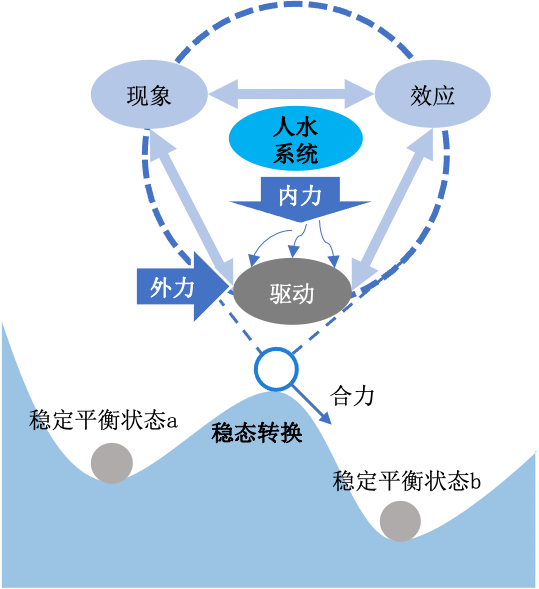
\includegraphics[width=0.5\textwidth]{img/ch2/ch2_framework.png}
    \caption{人水系统稳态转换的分析路径}\label{ch2:fig:identifying}
\end{figure}


\section{小结}\label{ch2:summary}
研究流域系统人\textendash{}水关系需要明确定义、范围和分析框架。
在流域尺度下,“人\textendash{}水关系”是一个存在尺度敏感性的概念,代表了利益相关者与水圈要素过程的联系状态。
为了研究方便,本研究将它定义为:在流域尺度下,主导人水复杂系统“自然\textendash{}社会二元循环结构”的利益相关者与地球表层系统中水圈要素过程的联系状态。
通过强调人\textendash{}水关系变化是流域系统反馈循环模式的重组,本章明确了稳态转换是识别人\textendash{}水关系变化的理论基础,识别稳态转换驱动力是理解作用机制的关键。
本章的定义和框架为流域人水研究提供了明确的方向,为分析其演变机制提供了关键的理论指导。


\label{chapter2}

\chapter{千年尺度的黄河流域人水关系演变}
\label{cha:3}


中国历史上长达3000多年的时间里,黄河流域一直是全国政治、经济和文化中心。
有说法认为“中国历史在某种程度上就是一部“治黄”史”,因为治理“善淤、善决”的黄河是历代中央王朝主导下人水关系的主旋律。
前人总结千年间历朝“黄河治理”的思想,认为虽先后有“堵”、“疏”、“分流”、“束水攻沙”等,但始终是着眼于河道的“治水为主”\cite{WangWeiJing2009}。
这种以“泥沙淤积”、“洪泛决溢”、“治水应对”所主导的人水关系,直到过去近百年间“从河道过渡至流域”的治理才得到改变。
近现代“水沙关系”的面上治理让黄河的年均泥沙排放量急剧下降至$0.1\sim0.2 Gt/yr$,有研究认为这个数字恰好与大约$2000$年前黄河原始的泥沙输送量相接近~\cite{wang2007}。
最近百年间的“水沙减少”的变化趋势已得到广泛研究\cite{wei2016, song2020, wang2016a},但对于过去$2000$年间,黄河水沙的变化过程何时发生、如何发生却尚缺乏系统认识。
于受人类主导之前黄河流域而言,梳理水沙关系变化对理解人水关系至关重要,因为水沙关系只是近代黄河流域治理的一部分,却是维系历史时期“泥沙淤积-洪泛决溢-治水应对”流域人水关系的核心。

% 黄河在距今$2000$年前仍处于较为原始的状态,其输沙量约为$0.1 \sim 0.2 Gt/yr$,仅为20世纪均值的十分之一\cite{xu2003a},黄河河道也相对较平稳,决溢灾害和治河活动相对较少(图\ref{fig:ch3:why_regime_shift})\cite{WangWeiJing2009, chen2012}。
% 但在$20$世纪以降,黄河流域已成为学界公认的、由人类主导“自然-社会二元水循环”的典型流域系统,“行洪输沙、生态环境、社会经济”多过程、多功能并重,由众多利益相关者共同组成了影响流域水循环的合力\cite{jiang2020b}。
% 但在历史时期,人类活动影响从微弱逐步变强大的过程中,黄河流域的人水关系一定经历了离开其原始稳态的过程,因为$2000$原始时期流域的生态环境与社会经济几乎不会在系统层面影响黄河,保障“行洪输沙”和社会安定是主要——甚至是利益相关者唯一的考虑。
% 在千年时间尺度上,除却气候的周期性波动,人类活动的影响虽总体呈增加趋势,也存在诸多非线性变量,因此识别“不可逆的结构重组”是识别稳态转换发生的关键标志\cite{GeQuanSheng2011}。

本章将流域系统“稳态转换”现象的分析框架应用在黄河,这些转换可能是由系统内部的渐进或累积性变化所引起,也可能是由人类或自然干扰所引起。
在$2000$余年前黄河流域的土地已开始被广泛地开垦使用,这一历史时期降水量主要由气候周期规律决定,但不断增强的人类活动导致黄河的泥沙排放总体呈现上升趋势\cite{wang2007}。
在历史时期,气候的变化和不断积累的人类活动双重作用对黄河由低输沙转化为高输沙状态的变化均有贡献,梳理其稳态转换何时、因何原因主导而发生,是理解人-水关系长时间尺度变化的重要基础。
研究昨日之黄河有助于理解今日之黄河,回望水沙关系的长时间尺度变化有助于在决策时看得更远。
本章就结合历史重建数据分析了过去两千年间黄河水沙排放的变化与其对流域的影响,特别关注历史时期黄河从原始水平到沉积物丰富水平的稳态转换,解析黄河流域脱离“泥沙淤积-洪泛决溢-治水应对”人水关系反馈关系的过程与机制。

% 黄河的频繁泛滥对中央王朝的治理带来严峻挑战,也积累有关黄河成灾的“集体记忆”。
% 史书累牍的黄泛之殇,是新中国成立伊始毛主席感慨“把黄河的事情办好”的动力,也可能是黄河人-水关系长期维持“洪水-响应”模式的内在机理。
% 这种有关长时间尺度的洪水灾害模型中,集体记忆已被认为是影响社会响应方式的核心变量之一~\cite{dibaldassarre2015, dibaldassarre2019,ciullo2017}。
% 因此,在识别稳态转换的基础上,使用集体记忆模型在气候周期波动变化下,预测人类社会对洪水的响应模式,是解释黄河长时间尺度上人-水关系演变的关键。

% 本章的研究首先从稳态转换的视角梳理了黄河从低输沙到高输沙的演变过程,从而区分周期性的气候驱动与不断积累的人为因素,继而利用洪水记忆模型解释了人类活动未突破稳态临界点之前,气候灾害的周期及集体记忆变化,是黄河人水关系在历史时期维持中央政府主导“洪水-响应”模式的内在机制。


\section{研究方法与数据来源}
\label{ch3:methods}
\subsection{研究路线与数据来源}
\label{sec:ch3:method}


距今$2000$年前,在人类干预较低的时期,尽管已获“黄河”之名,但这条中华民族的母亲河相较当今仍处于非常原始的状态(图\ref{fig:ch3_why_regime_shift}~A)。
Xu等人(2003)\cite{xu2003a}指出,当时黄河输沙量约为$0.1\sim0.2 Gt$,仅是20世纪均值的十分之一;Chen等人的研究(2012)\cite{chen2012}与王渭泾(2009)\cite{WangWeiJing2009}的著作也指出,黄河河道彼时正处于长时间较平稳的状态,决溢灾害、治河活动也相对较少。
但在20世纪以降,黄河流域几乎已成为学界公认的、是由人类影响主导水循环模式的典型代表,其人-水关系模式被总结为“行洪输沙、生态环境、社会经济”并重综合的复杂系统\cite{jiang2020b}。
因此,与寻找“人类世”的起点有异曲同工之妙,本章研究将假设历史时期人水关系的与近期(百年尺度)是不同的,设计方法在千年尺度上定量识别黄河人-水关系的稳态转换,并分析稳态转换前的人水关系模式。

具体来说,本章研究重点包括以下两个:
(1)识别黄河流域在历史时期内典型稳态转换的发生过程(图\ref{fig:ch3_why_regime_shift}~B)。
稳态转换的发生以“不可逆的大规模结构重组”的发生为标志,而在千年时间尺度上,气候多呈现周期波动的趋势,人类活动的影响总体呈持续增加趋势,且人口、治理、土地利用等变化大多是非线性的\cite{GeQuanSheng2011}。
因此,识别人-水关系稳态转换的关键是将气候的周期性变化、日益增长的人类活动压力各自对流域系统的影响相剥离,并识别人类活动驱动因素超越气候周期波动影响的时期。

(2)分析在该稳态转换发生前,黄河流域人水关系的模式(图\ref{fig:ch3_why_regime_shift}~C)。
根据本研究在\ref{ch2:definitions}\nameref{ch2:definitions}中所下的定义,对人水关系模式的总结需要考虑“决定社会-水文循环的利益相关者是谁”,以及“该利益相关者的认知或行动模式是怎样的”等问题。
由于历史时期可获取的数据或记载的局限性,研究中将利益相关者简单分为“中央政府”与“大众”,其影响社会-水文过程的主要因素分别是对河流的治理,以及对土地利用-覆被的改造。
因此,总结此时期人-水关系的关键,是在千年时间尺度下分析上述因素是否对社会-水文反馈循环产生明显影响。

\begin{figure}[H] % use float package if you want it here
    \centering
    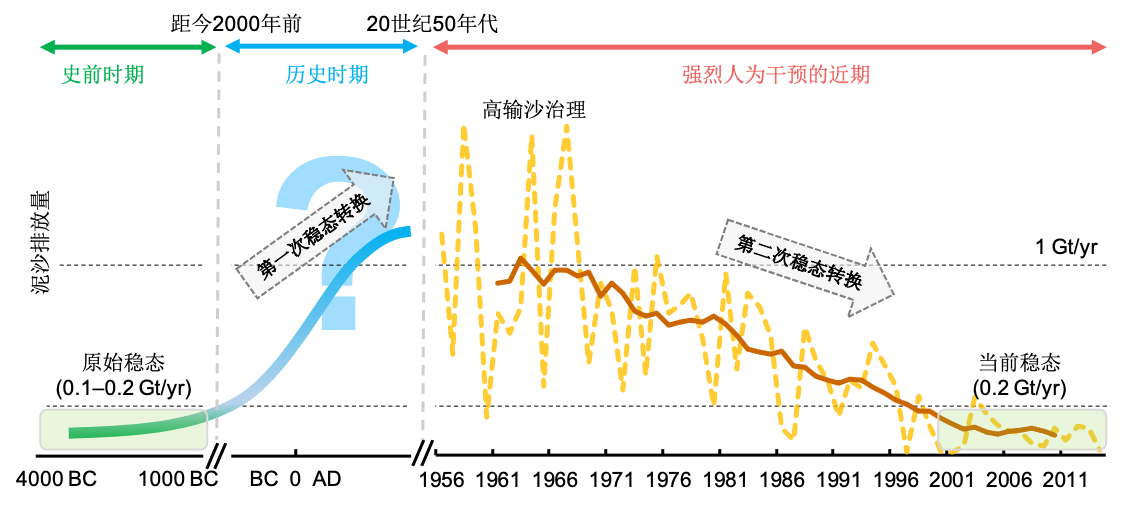
\includegraphics[width=\textwidth]{img/ch3/ch3_why_regime_shift.png}
    \caption[黄河流域千年尺度人-水关系变化的关键研究问题]{黄河流域千年尺度人-水关系变化的关键研究问题。第一次稳态转换发生在历史时期}
    \label{fig:ch3_why_regime_shift}
\end{figure}

此外,数据是开展历史时期研究的主要挑战,上述研究路线须根据可获得的、质量可靠的数据来设计具体方法和指标。本研究通过整理前人在沉积学、气候学、历史学等领域的著述,获取到公开发表、质量可靠的数据及其来源如表\ref{tab:data_source}所示。

% Table generated by Excel2LaTeX from sheet 'Sheet1'
\begin{table}[hbt]
  % \centering
  % \begin{minipage}[t]{0.8\linewidth}
  \caption[千年尺度黄河稳态转换识别的数据来源]{千年尺度黄河稳态转换识别的数据来源。}
    % \begin{tabular}{llllll}
    \begin{tabularx}{\textwidth}{ p{2cm} L p{5cm} L p{3cm} L}
    \toprule
    数据集   & 类型    & 描述    & 原始材料  & 可信度   & 参考 \\
    \midrule
    干旱和洪涝频率 & 气候驱动力 & 每五十年为一个时期,分别统计中原、华北平原地区的干旱、洪涝灾害的频次 & 官方和地方的史料记录 & 根据历史材料的丰富程度,在不同时期的可信度是不一致的 & 葛全胜,2011 \cite{GeQuanSheng2011} \\
    湿润指数累计距平 & 气候驱动力 & 根据史料中与湿度相关的记录,评估历史时期气候湿润程度的等级 & 官方和地方的史料记录 & 根据历史材料的丰富程度,在不同时期的可信度是不一致的 & Zheng,2006 \cite{zheng2006} \\
    黄河中游人口数量 & 人类活动驱动力 & 利用史料记录推断的黄河中游人口 & 历史户籍注册信息 & 数字不精确但可以反映趋势以供纵向比较 & Chen et al., 2012 \cite{chen2012} \\
    农牧交错带的北界位置 & 混合驱动力 & 农牧交界线距离潼关所在维度的平均距离 & 中国历史地图集 & 时间采样点比较少,但每个点的位置数据较为可信 & 谭其骧,1996 \cite{TanQiXiang1996} \\
    三门峡峡谷航运数据 & 影响$^*$    & 三门峡航运通行难易程度的等级 & 官方和地方的史料记录 & 数据从可靠的史料来源获得,但存在数据缺失情况 & 王守春,1993 \cite{WangShouChun1993} \\ %TODO 这里还需要参考,查证王老师那的书
    黄河下游决溢数据 & 影响    & 黄河下游堤防崩溃的次数 & 官方和地方的史料记录 & 根据历史材料的丰富程度,在不同时期的可信度是不一致的 & Chen et al., 2012 \cite{chen2012} \\
    黄河古河道沉积速率 & 影响    & 结合历史地图和取样测定的黄河古河道沉积速率 & 沉积样本  & 样本所在的古河道时间跨度越长样本越精确 & Xu 2003 \cite{xu2003a} \\
    \bottomrule
    % \end{tabular}%
  \end{tabularx}\\[2pt]
  % \leftalighn
  \footnotesize 注:*影响:指黄河关键特征变化带来的影响。\\\label{tab:data_source}%
  % \end{minipage}
\end{table}%



\subsection{稳态转换过程的识别途径}
\label{sec:ch3:approach}

在历史时期的黄河流域,由于缺乏对流域的系统性认识,不断增长的人为压力带来的影响主要是中游黄土区的开垦进而导致输沙量的提升\cite{wu2020a}。
针对此次稳态转换的特点,分析其发生过程的关键是识别黄河输沙量的变化与气候周期“脱钩”的时段,因此本研究设计了如图\ref{fig:ch3_regime_shift_detect}所示的稳态转换识别框架。
周期性气候变化和不断增长的人为因素(主要是中游易侵蚀区的粮食生产)共同驱动着产沙量、产水量两个关键特征的变化,二者的变化则会在流域内触发一系列影响因素变化。
在气候湿润时期,土壤侵蚀和径流增加了更丰富的降水,会导致产水量和产沙量同时增增加,因此二者也存在一定的正相关关系。
但而随着人类活动压力增大,开垦造成粮食产量增通常减少植被的覆盖范围,从而加剧水土流失,这主要导致产沙量增多。
因此通过分析与产沙过程、产水过程关系有所差异的三类影响因素变化趋势(图\ref{fig:ch3_impacts}),理论上可以找到“产沙量增加比产水量增加更显著”的关键变化时期。

% 总体潮湿的气候让宋代农牧交错带北移,但极端气候增多,干旱造就了土地退化,洪水增加了侵蚀,平水年份水量较多。
% 清朝乾隆之后航运断绝,平水时期的三门峡河道都难以行船了,这或许是明清黄河输沙持续恶化的体现。
% 由于直接证据的缺乏,河道兴废、三角洲扩张,结合决溢材料,三者结合起来才能说明河道的沉沙情况。

\begin{figure}[H] % use float package if you want it here
    \centering
    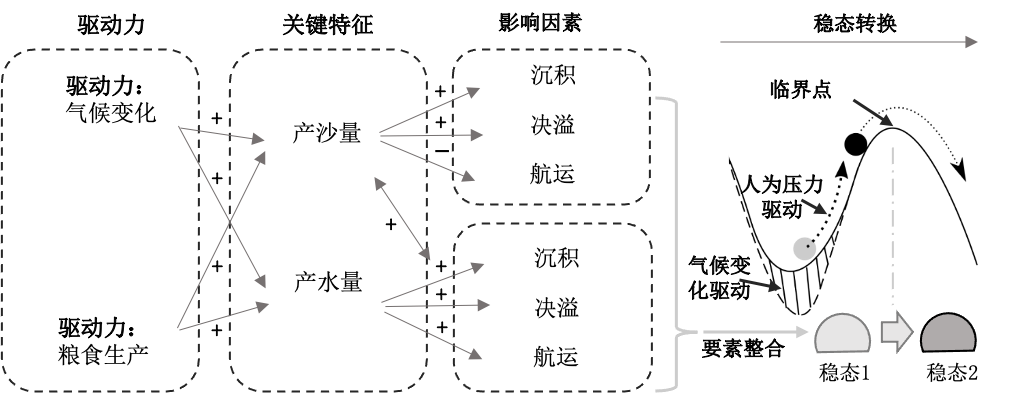
\includegraphics{ch3/ch3_workflow.png}
    \caption[黄河历史时期稳态转换识别的框架]{黄河历史时期稳态转换识别的框架。气候变化和粮食生产是致使稳态转换发生的潜在驱动力;稳态转换发生时影响的关键是产沙量和产水量;二者的变化又会触发流域一系列影响因素变化。灰色箭头及其旁边的符号表示消极或者积极的影响路径;在驱动力推动系统接近临界点时,所有受影响因素经整合后会展示稳态转换是否发生。}
    \label{fig:ch3_regime_shift_detect}
\end{figure}

\begin{figure}[H] % use float package if you want it here
    \centering
    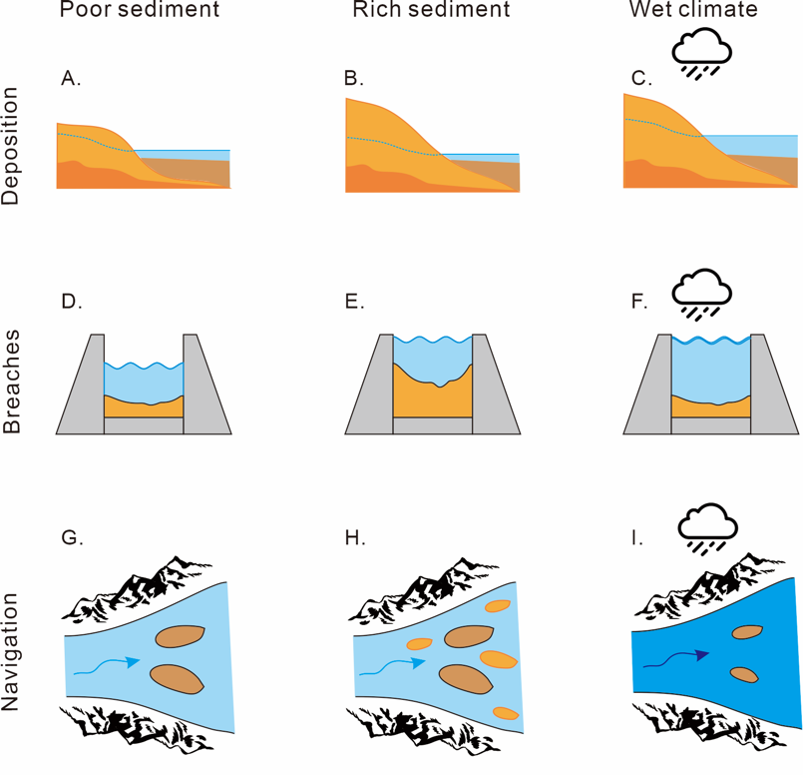
\includegraphics{img/ch3/ch3_impacts.png}
    \caption[黄河历史产水量和产沙量带来的影响]{黄河历史产水量和产沙量带来的影响。输沙和产水两个主要特征分别对沉积(A-C);决溢(D-F);航运(G-H)的影响。
    (1)对于沉积数据,产沙量高(从A到B)可能导致下游沉积速率增加\cite{xu2003a};
    (2)对于洪泛数据,产沙量高(从D到E)或者气候湿润期(从D到F)都有可能导致更多的决溢洪泛\cite{chen2012};
    (3)对于航运数据,产沙量高(从G到H)会增加浅滩数量,从而使航运变得更加困难,而潮湿的气候时期由于平均径流量变大,三门峡的通航将更加容易\cite{WangShouChun1993}。}
    \label{fig:ch3_impacts}
\end{figure}

用以分析稳态转换驱动因素的数据集匹配本研究需要,均不做进一步处理,而反映黄河特征变化带来的影响的三个数据集(黄河古河道沉积速率、洪泛决溢次数、三门峡航运情况)按表\ref{tab:ch3_impacts_magnitude}进行半定量化。
此外,由于历史资料难以避免具有不确定性,需依据上述三个数据集各自特点评估其置信度并进行整合。
我们先分别对沉积、决溢、航运三个数据集各自的置信度按公式\ref{eq:ch3_credibility}所示方法进行估计:
(1)由于沉积每个数据是对遗留河床样本的平均估计,遗留时间越长的古河床样本所估计值相对可靠;
(2)溃堤数据的置信度取决于官方史料的可靠程度,该时期的历史记录更可靠、存留的历史记录更多,则该时期的估计值也更可靠;
(3)航运数据出处未给出各时段的史料置信度,所以该数据的置信情况使用时段内航运相关记录的数量进行评估。
最后,再将每个数据集置信度按极大-极小归一化(公式\ref{eq:ch3_normalize})后同样划分为三个置信等级。

% Table generated by Excel2LaTeX from sheet '影响强度半定量化'
\begin{table}[!htbp]
    \caption{黄河关键特征变化影响强度的半定量分级}
      \begin{tabularx}{\textwidth}{p{1.5cm} LLL}
      \toprule
      \multicolumn{1}{l}{强度等级} & 古河道沉积速率 & 洪泛决溢频次 & 三门峡航运情况 \\
      \midrule
      1     & $0 \sim 2$ cm/yr & < 10次 / 20yrs & 自由通行 \\
      2     & $2 \sim 4$ cm/yr & 10~20次 / 20yrs & 需要人力辅助 \\
      3     & $\> 4cm/yr$ & >20次 / 20yrs & 完全无法通行 \\
      \bottomrule
      \end{tabularx}%
    \label{tab:ch3_impacts_magnitude}%
\end{table}%


\begin{equation}
    \label{eq:ch3_credibility}
    Credibility_X = 
    \left\{\begin{array}{l}
        \text{[沉积], } 1 / \frac{1}{n} \sum_{i=1}^n T_i\\
        \text{[决溢], } \prod_{i=1}^n C_i\\
        \text{[航运], } N_i
    \end{array}\right.
\end{equation}

其中$n$均为给定时段内各数据集样本/记录的数量。$T_i$为每个沉积样本所在古河道的时间跨度;$C_i$是每个历史记录所在时段的置信程度(由数据作者给出的评估,详见表\ref{tab:data_source});$N_i$是每个时期航运相关历史记录的数量。

\begin{equation}
    \label{eq:ch3_normalize}
    C_{nom}=\frac{C-C_{\min}}{C_{\max}-C_{\min}}
\end{equation}

其中$C_{X}$为参照公式\ref{eq:ch3_credibility}对数据集$X$进行评估后的置信程度,$C_{\min, X}$, $C_{\max, X}$分别为数据的最小值和最大值。$C_nom$为归一化后的置信程度。

\subsection{稳态转换过程的分析方法}

基于\nameref{fig:ch3_regime_shift_detect}的解释框架,我们首先识别不同驱动力(潮湿气候/人类活动)所主导的时段,再分析该时段之前、之中、之后受到影响的指标如何变化。
因为干燥和潮湿的气候在中国往往以$\sim100$年为周期\cite{GeQuanSheng2011},我们以100年最低阈值来检测气候驱动时段(Climate-driven Periods, CDPs)。
我们将分别能反映潮湿环境和极端降水的湿度数据和洪水频率数据作为识别过去两千年中历史气候驱动时段出现的指标。
因此,在每个$100$年时段中,若洪水的频次高于干旱事件频次,且累积湿度距平在上升,则可以认为是典型的气候驱动时段。

人类活动带来的主要压力来自于黄河中游的人口增长以及农业扩张。
尽管目前没有精确的人口数据,但是中国历史人口变化的趋势已在一些基于户籍统计的历史重建资料中得到反映(见表\ref{tab:data_source})。
此外,农牧交错带北界的移动也是人类活动的重要特征,我们将其作为人类活动驱动时段(Human-driven Periods)的辅助识别指标。
因为人口的增长不一定直接伴随农业开垦面积的扩张,仅当同时发生农业人口增长和农牧交错带北界的移动时,才能认为是人类活动驱动时段。

在识别出气候驱动时段和人类活动驱动时段后,我们将分析这些时段对是否可能发生黄河输沙量变化与气候周期“脱钩”的情况(正如\ref{sec:ch3:approach}\nameref{sec:ch3:approach}中所述,本研究认为其指示着稳态转换的发生。

\subsection{人水关系反馈回路识别}
% 以及缺乏系统性地“只关注河道”的河流治理模式\cite{WangWeiJing2009}


\section{历史时期稳态转换发生过程}
\label{ch3:process}

\subsection{稳态转换潜在驱动期识别}

根据气候湿润与人类活动两类驱动因素的组合,本章研究将黄河在历史时期的驱动因素变化过程分为七个时期(表\ref{tab:ch3:periods_division})。
在公元400年之前,由于所有原始数据的可信度均较低,因此本研究不再后续分析中讨论(图\ref{fig:ch3:drivers}~A)。
过去的2000年间,研究区的大多数时期均偏干燥,记录了223次极旱年和182个洪泛年,因此强烈湿润的气候驱动时段较少。
结合湿润指数,本章研究为黄河流域在过去两千年中识别出三个潜在的气候驱动期(CDPs),其中有两个在数据可靠的时期,分别开始于900AD和1700AD(图\ref{fig:ch3:drivers}~B)。
另一方面,在公元900年之前几乎没有人类活动驱动的迹象(图\ref{fig:ch3:drivers}~C)。
虽然900AD-1000AD间农业区域向北扩大可能指示人类活动的增强,但由于缺乏可靠的人口增长证据,且气候暖湿化也会引起农区扩张,所以此时段在本研究中不被认为是一个确定的人类活动驱动时段(HDP)。
而在这之后的1450年至1650年以及1900年后,随着人口显著增加和农牧交错带向北移动,本研究将这两个时段认为是需要分析的人类活动驱动时期(HDPs)。

% Table generated by Excel2LaTeX from sheet '历史时期特征划分'
\begin{table}[htbp]
    \centering
    \caption{基于驱动因素的历史时段划分及其特点}
      \begin{tabularx}{\textwidth}{LLL}
      \toprule
      时间跨度  & 时段划分  & 主要特征 \\
      \midrule
      200BC-400AD & 数据不可信时段 & 各数据集在此时期的可信度均偏低 \\
      400-900AD & CDP1前期 & 没有明显的驱动因素 \\
      900-1100AD & CDP1时期 & 气候驱动与低水平的人类活动驱动时期 \\
      1100-1350AD & CDP1后期 & 没有明显的驱动因素 \\
      1350-1700AD & CDP2前期 & 人类活动驱动时期 \\
      1700-1900AD & CDP2时期 & 气候驱动与人类活动共同驱动时期 \\
      1900-2000AD & HDP2时期 & 人口迅速增长的人类活动强烈驱动期 \\
      \bottomrule
      \end{tabularx}%
    \label{tab:ch3:periods_division}%
\end{table}%
  

% \begin{rotate
\begin{figure}[!ht]
    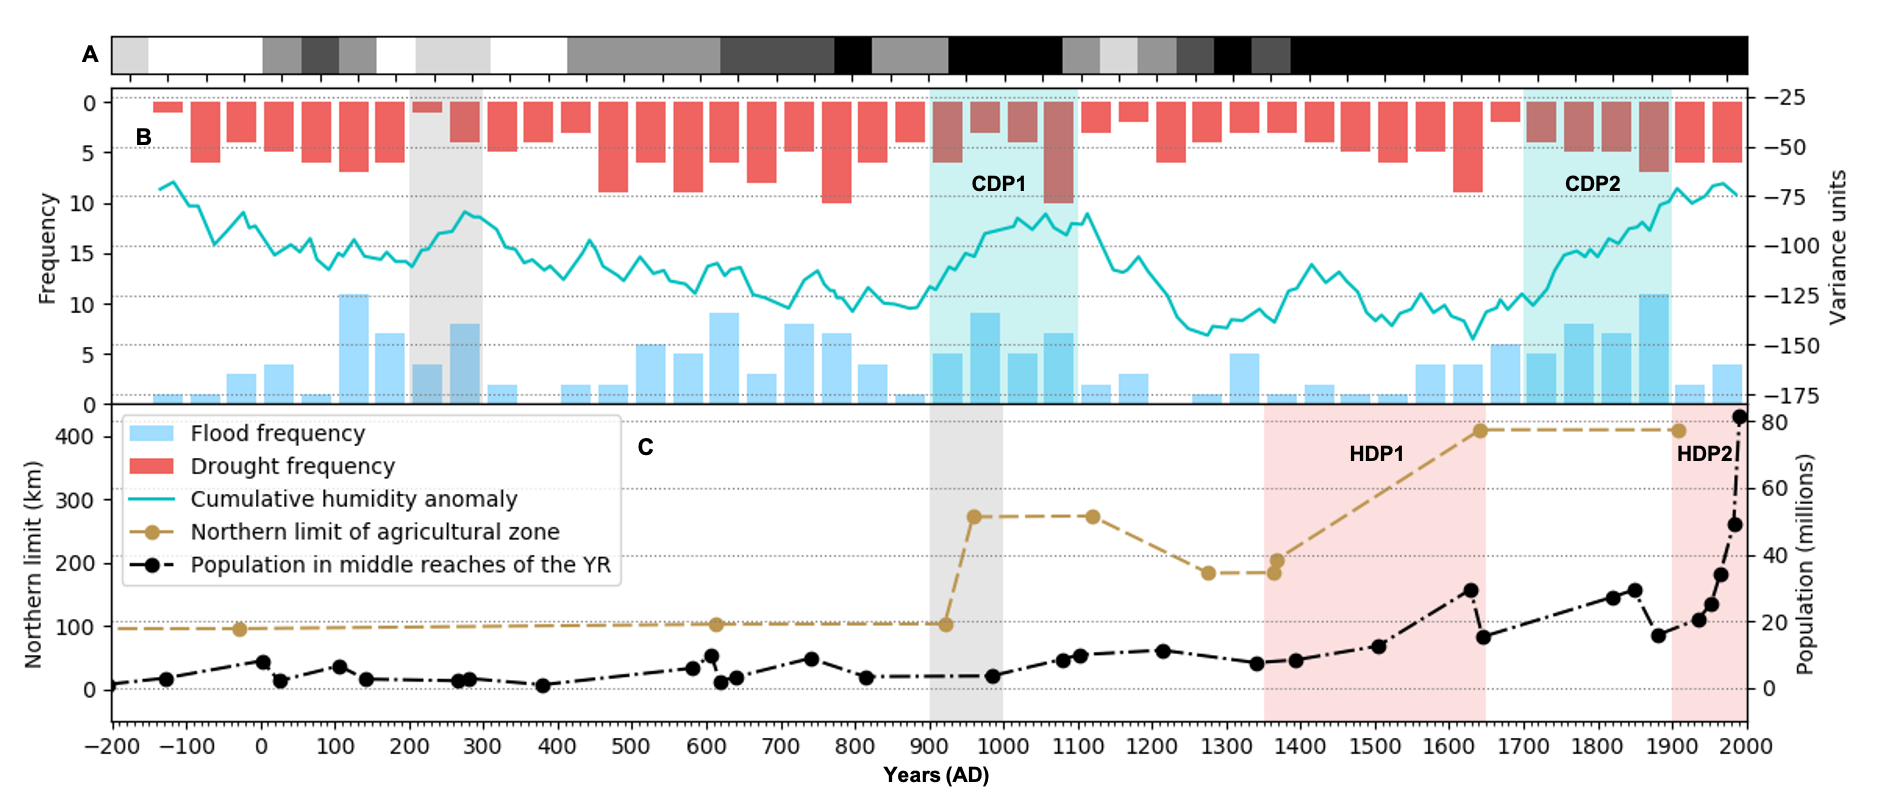
\includegraphics[width=\textwidth]{img/ch3/ch3_drivers.png}
    \caption[黄河流域历史时期稳态转换的驱动力变化]{黄河流域历史时期稳态转换的驱动力变化。
    \textbf{A} 原始数据有五级综合置信度(1 - 5),分别从极低置信度(白色)到极高置信度(黑色);
    \textbf{B} 气候驱动时期:用极端气候频率(干旱或洪水)以及累积湿润度距平共同确定的两个明显的气候驱动时段(CDPs),由蓝色阴影表示;
    \textbf{C} 人类活动驱动时期:根据黄河中游人口增长和农牧交错带北界的移动情况确定的人类活动驱动时段(HDPs),由红色阴影表示$^*$。}
    \footnotesize
    * 灰色阴影的部分表示农牧交错带北极界移动,但因缺乏可靠的人口增长证据且气候湿润也会引起农区扩张,所以不认为是一个人类活动驱动时段(HDP)。\label{fig:ch3:drivers}
\end{figure}

\subsection{稳态转换的影响因素变化}

根据上述时段划分,自CDP1开始(图\ref{fig:ch3:impacts}~CDP1),黄河的决溢现象更加频繁,三门峡通航也变得更容易,同时下游两个样品的沉积速率也超过了$4cm/yr$,显示出湿润气候驱动力的影响。
然而在CDP1之后,尽管没有通过沉积样品评估泥沙量,但洪泛频率的降低与重新变差的航运情况表明,黄河的情况重新回到了CDP1之前的时期。
最后,在进入第一个明显的人类驱动时期(HDP1)时,更多的沉积样品表现出下游泥沙沉积速率明显上升的趋势(图\ref{fig:ch3:impacts}~HDP1-HDP2),并伴随更频繁的洪泛和持续糟糕的航运水平。


根据数据的可信度,图\ref{fig:ch3:impacts}提供了两个气候驱动期(CDP)前、中、后期的情况对比。
首先,直接反映输沙量的沉积率指标在HDP1之后的可信度一直较低,直到第二个人类驱动时期(HDP2)结束后才有较为可靠的增加证据(图\ref{fig:ch3:impacts}~E和F)。
其次,尽管这两个湿润的气候驱动时期都让洪泛频率明显增加(图\ref{fig:ch3:impacts}~D和E),但只有在第一个气候驱动期(CDP1)时航运更加便利,而在第二个气候驱动期结束后(CDP2,恰好也是人类活动强烈驱动期 HDP2)反而航运更加困难了。
综上所述,虽然气候存在周期性,但第一个强烈的气候驱动期(CDP1,900AD - 1100AD)和第二个气候驱动期(CDP2,1700AD - 1900AD)已呈现出不同的流域系统过程。

\begin{figure}[!ht] % use float package if you want it here
    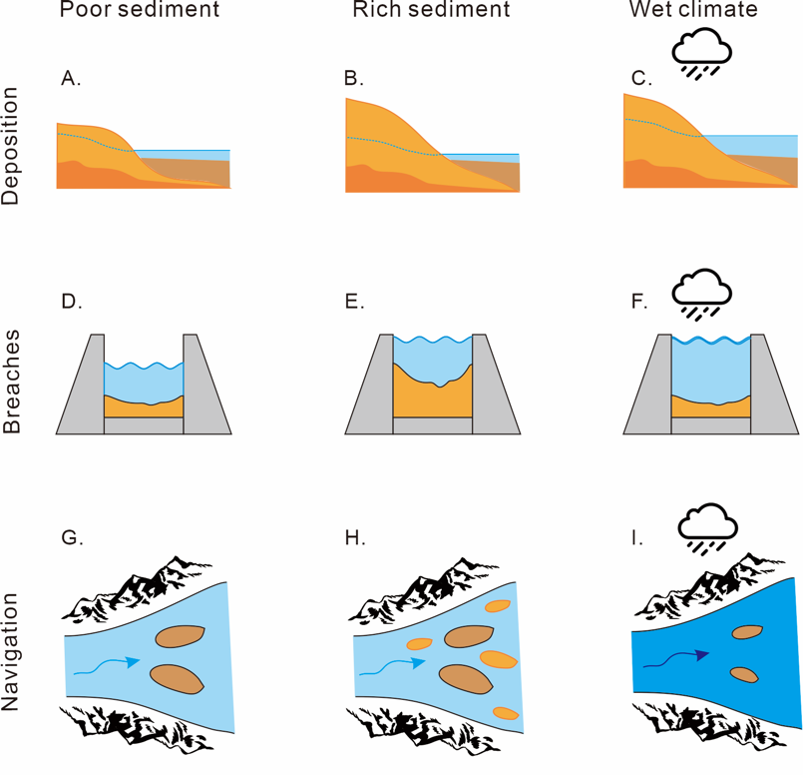
\includegraphics[width=\textwidth]{img/ch3/ch3_impacts.png}
    \caption[历史时期各时段的影响因素与信度变化]{历史时期各时段的影响因素与信度变化。每个时段内(气候驱动时段CDP,或人类活动驱动时段HDP),沉积(黄色)、洪泛(蓝色)、航运(红色)三个典型受影响因素的特征等级与可信度等级(见\ref{sec:ch3:approach}\nameref{sec:ch3:approach})。
    在每个半圆内,扇形的半径表明影响因素的强度等级,弧长表示其数据可信度。由于航运和洪泛滥同水量变化是相反的,本章研究将它们放在扇形的不同象限,从而使扇形左右两个方向分别代表更少的水量与更多的水量。简而言之,某个颜色的扇形面积更大,就有越大的把握说明该时段内的此影响因素强度。A - F分别代表被两次气候驱动期CDP所分割的不同时段: (A) 400AD - 900AD (B) 900AD - 1100AD (C) 1100AD - 1350AD (D) 1350AD - 1700AD (E) 1700AD - 1900AD 和 (F) 1900AD - 2000AD。}\label{fig:ch3:impacts}
\end{figure}



\section{稳态转换前黄河人水关系模式}
\label{ch3:mechanism}

\section{讨论}

% 总体潮湿的气候让宋代农牧交错带北移,但极端气候增多,干旱造就了土地退化,洪水增加了侵蚀,平水年份水量较多。
% 清朝乾隆之后航运断绝,平水时期的三门峡河道都难以行船了,这或许是明清黄河输沙持续恶化的体现。
% 由于直接证据的缺乏,河道兴废、三角洲扩张,结合决溢材料,三者结合起来才能说明河道的沉沙情况。


由于研究时段较长,本章使用的数据集是历史记录、历史时期重建数据、估算数据 以及 1949 年之后观测和统计数据的组合(表 2.1,2.2)。历史记录和重建数据高度依赖 相关典籍和文献的准确性,但由于隐匿和漏报等问题,一些历史档案中可能存在错误 或不确定性(葛全胜等, 2003)。而本章用到的历史时期估算数据也是来自其他研究根据 相关文献典籍或相关资料(如沉积速率等)的估算,虽然存在一定不确定性,时间分辨 率也有限,但指标的变化趋势基本可信。本章用到的大部分历史数据集是相应指标的 仅有的数据源,虽然对这些数据的可靠性持谨慎态度,我们还是相信本研究基本体现 了黄土高原社会-生态系统变化的总体趋势。

\section{小结}
\label{chapter3}

\chapter{百年尺度的黄河流域人水关系演变}\label{cha:4}
第三章研究表明,人为压力和气候变化因素仅触发了黄河泥沙量的稳态转换,黄河流域在千年尺度上是由层级制度主导的“洪泛-响应”关系。除此之外,非中央政府主导的开发利用、生产贸易、综合治理等因素,尚没有显著影响人水关系稳态。而现代黄河流域人水关系出现的关键变化之一就是对黄河流域全面的综合开发、利用、以及治理。黄河流域的战略瓶颈已经由保护黄河泛滥转向应对高质量发展面临的水资源短缺、人水关系不协调问题之上。第三章研究已经表明,这是19世纪以降短短百余年间经济社会高速发展带来的问题,而新中国成立以来,高强度的黄河流域综合治理,使得近六十年间黄河流域人水关系的演变模式与过去千年相比显得截然不同。

首先在流域内部,积累的取水压力让这个位于干旱-半干旱区的流域迅速不堪重负,取水量一度接近年径流的$80\%$,其中近$90\%$均为农业取水。因此,黄河自1970年代开始频繁断流,这引起中央高度重视,开始采取一系列水资源管理的工程、非工程措施来协调水资源供需矛盾。与此同时,大规模的经济建设和城市发展也让宝贵水资源的流域内分配成为了挑战。而跨区域贸易带来了水资源以农产品形式向流域外的转移,让水资源分配的问题变得更加复杂严峻。因此,黄河流域已从过去的调水调沙与防洪等河道内外的“工程问题”,转向了“谁、在何时得到水”的流域层面的“非工程问题”,这是近现代人水关系演变的体现。而这种稳态转变何时发生、如何发生,仍需要定量研究。本章在黄河流域市级统计数据的支持下,利用断点识别、复杂网络分析等方法量化分析了上世纪七十年代以来的黄河人水关系演变过程及驱动因素。

黄河流域是世界上第五大、最富沉积物的河流,由于地质和人类历史的原因,需要综合的水治理
\cite{mostern2021,best2019}。
自20世纪60年代以来,水库、堤坝和保护措施等治理措施已经遏制了数千年来高沉积物负荷所困扰的问题
\cite{wang2016e,song2020a}。
然而,最近出现了新的挑战,如流量减少和水资源枯竭,导致了用水调节和跨流域的水转移——不同的重点水治理策略
\cite{wang2019c}。
目前,还不可能完全解决长江流域水资源压力、生态系统服务之间的权衡、不同区域的不平衡发展问题,使各方都满意
\cite{wohlfart2016a}。
由环境、经济、社会和政治因素引发的治理挑战导致长江流域成为世界上治理最密集的大型流域之一。
因此,确定长江流域内水治理的政权变化,可以为快速变化的大流域以及治理如何应对其可持续性挑战提供重要的见解。

\section{研究方法与数据来源}\label{ch4:methods}

\subsection{分析框架}

% 根据本研究的定义,人类活动主导下的人\textendash{}水关系是社会\textendash{}水文二元循环中由人类主导的决策模式
% 而水治理(Water Governance)是指影响水使用和管理的政治、社会、经济、和行政系统相互作用的全部过程,本质上是关于``谁获得水,何时获得水,如何获得水''(``who gets water, when and how'')。
联合国开发计划署(UNDP)提出\cite{mariajacobson2013},水治理决定了与水有关的三个核心方面:``什么时候有多少水用?''、``水如何为人类福祉提供不同的生态系统服务?''以及``谁能平等有效地用水?''——简而言之,水治理是决定水资源``稀缺情况''、``使用目的''、和``分配方式''的关键。
为此,本章研究将水治理的三个核心方面(``稀缺情况''、``使用目的''和``分配方式'')各自选择指标进行量化,对它们进行等权平均得到综合水治理指数(Integrated Water Governance Index, IWGI)用以识别水治理的稳态变化(图\ref{ch4:fig:framework})。
然后,通过将该指数应用在黄河这个典型的人类活动主导的流域,利用突变点检测的方法分析了$1965\sim2013$年间IWGI的变化,展示该IWGI如何有助于检测和描述复杂的水治理稳态变迁。
最后,在综合分析了水资源供需、经济发展、环境变迁,以及制度变化后,本章解释了黄河流域水治理稳态变化的主要驱动因素,并总结提出了一个过渡模式,为人类活动主导大河流域面临的治理挑战提供了抓手。

\begin{figure}[!ht]
\centering
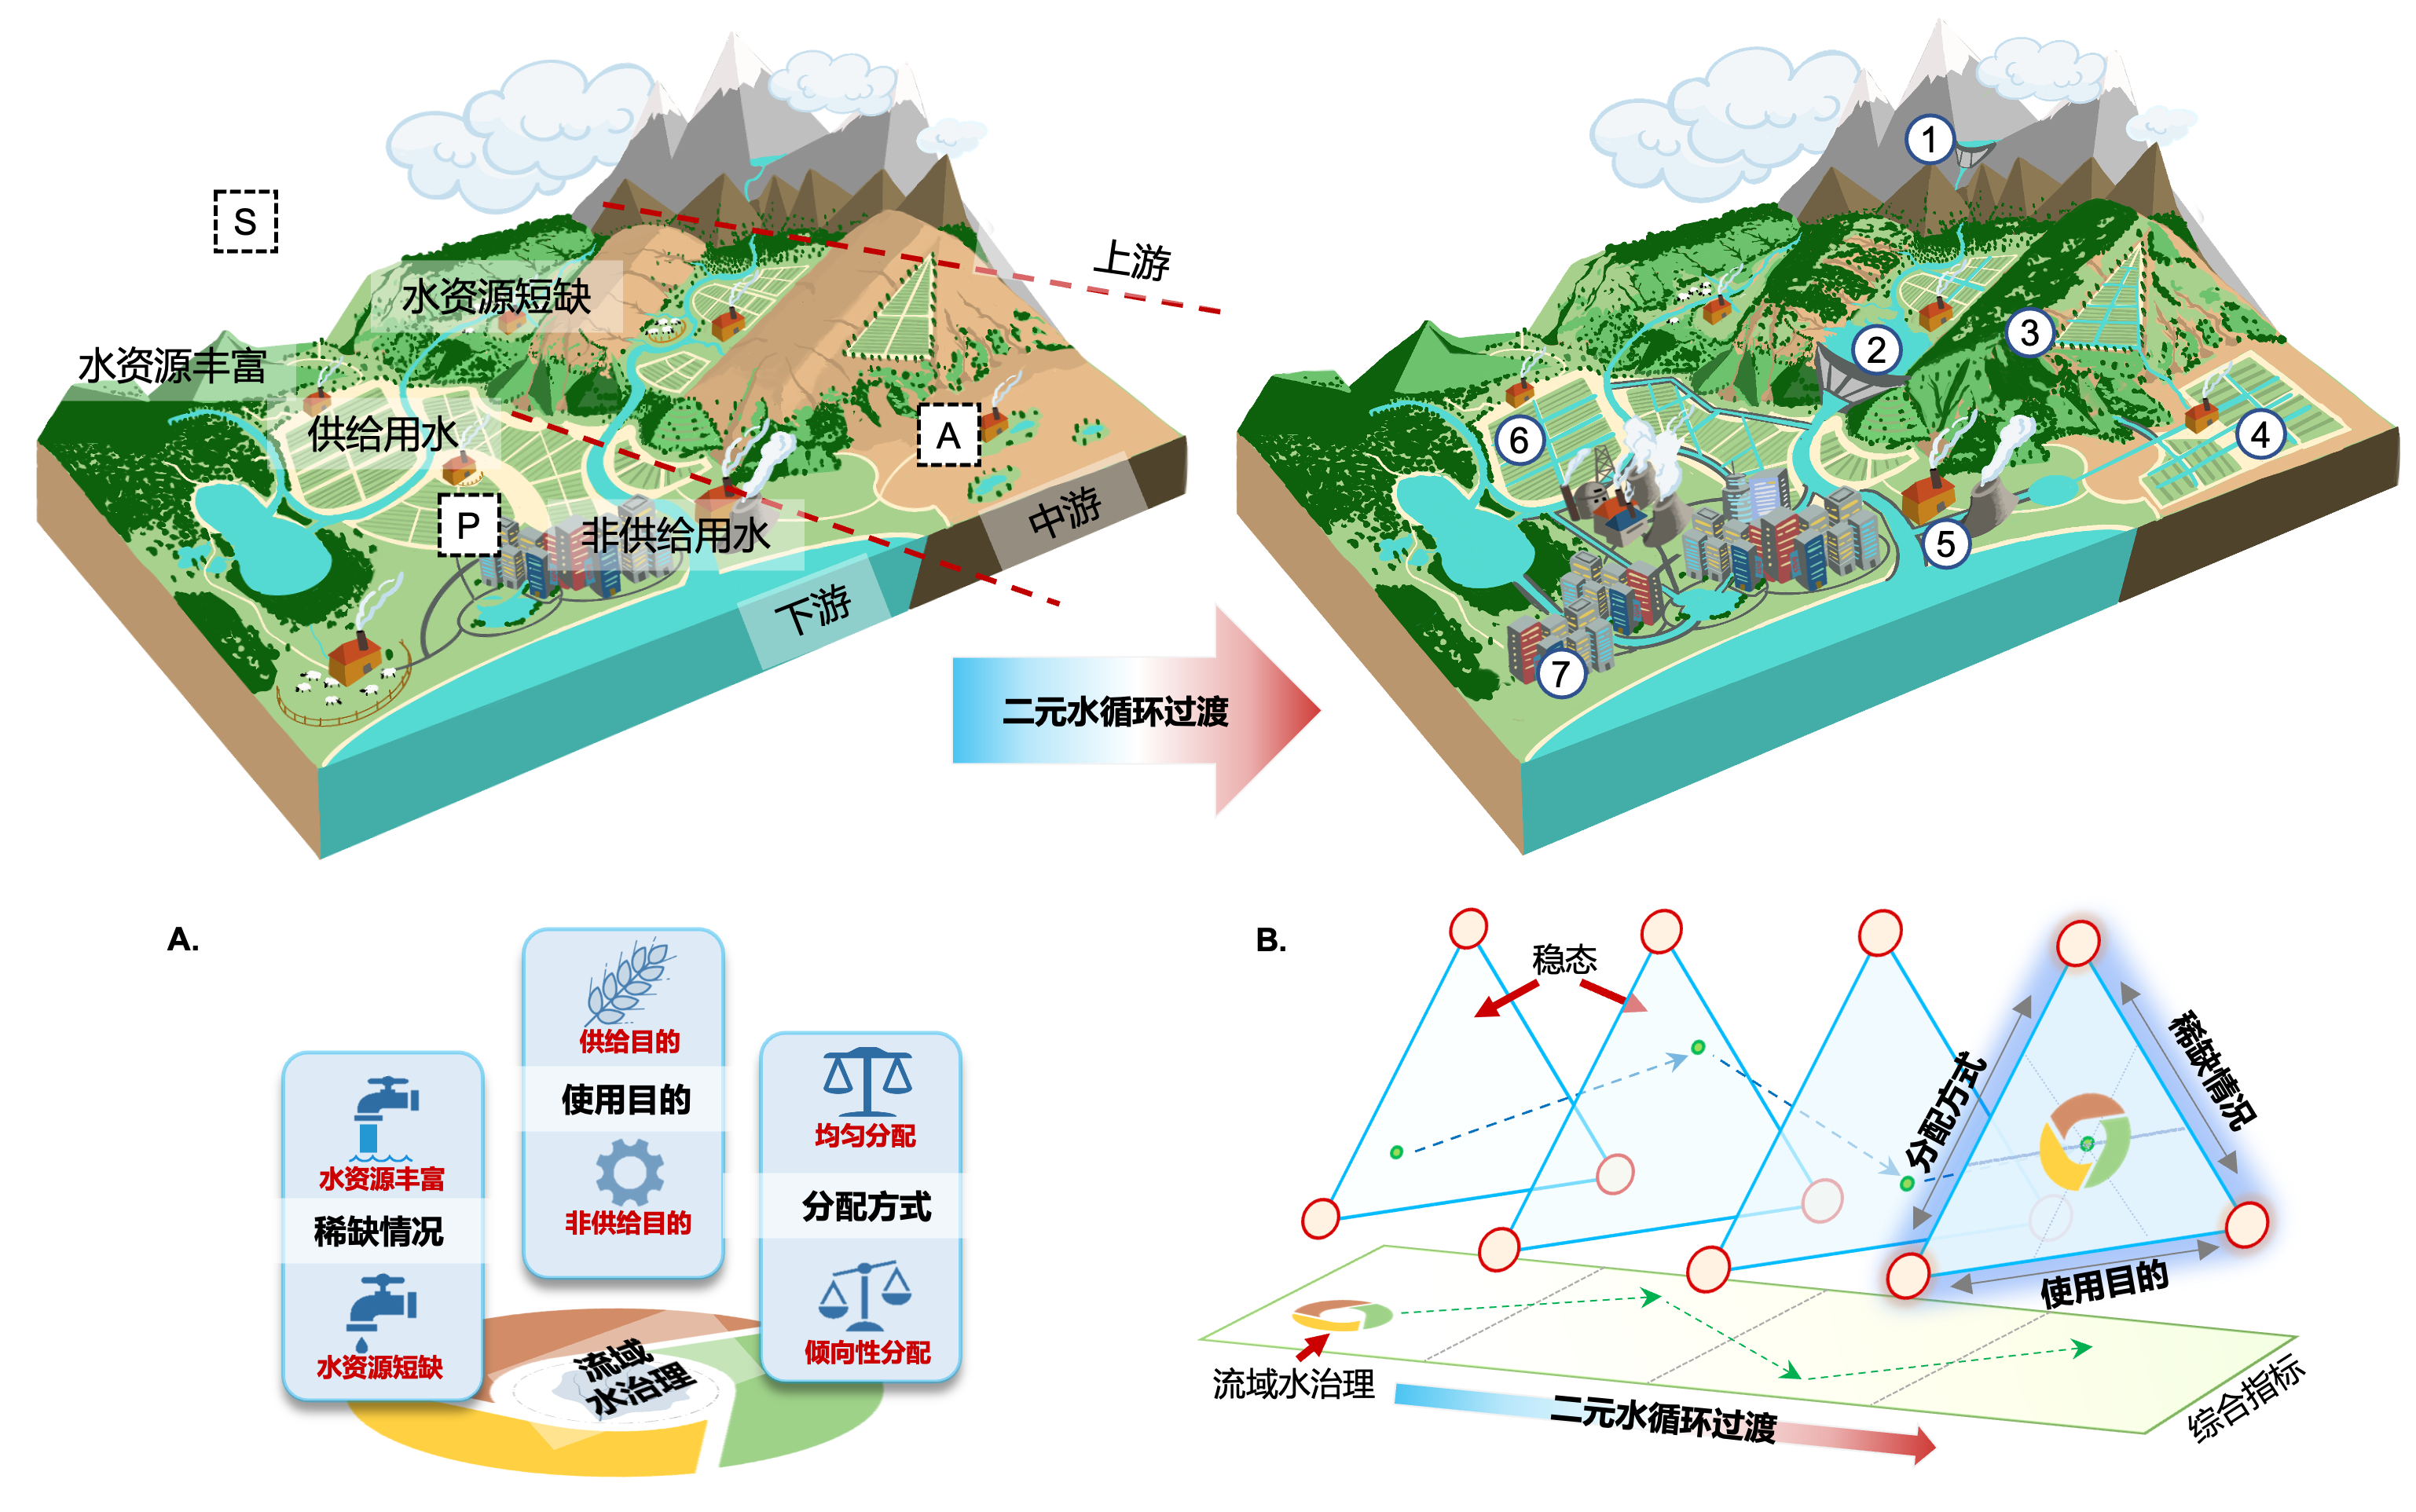
\includegraphics[width=\textwidth]{img/ch4/ch4_framework.png}
\caption[定量识别流域水治理转变的分析框架]{
    定量识别流域水治理转变的分析框架。
    \textbf{A} 利用综合水治理指数(IWGI)识别水自然\textendash{}社会二元循环过渡时期中的水治理机制,可以从稀缺情况(S)、使用目的(P)和分配方式(A)这三方面切入,三者会随着人类活动主导社会\textendash{}水文循环而变化。
    例如,水库建设(\ding{172}和\ding{173})可以缓解局地水资源压力;集约化灌溉农业的发展(\ding{174})以及能源和工业增长(\ding{175})会改变水的利用方式;输水系统控制了流域系统的水分配(\ding{176}和\ding{177})。
    \textbf{B} IWGI方法结合三个方面的相应指标,因此其突变可以指示水治理的稳态转换。}\label{ch4:fig:framework}
\end{figure}

\subsection{研究区域划分}\label{ch4:sec:region}

为便于研究的计算需要,本章参考前人研究和黄河水利委员会的标准将黄河流域划分为四个区域\cite{shuilibuhuangheshuiliweiyuanhui2010,wang2019c},以四个重要的控制水文站反映各区域的径流变化,各区域特点鲜明,便于后文对水资源治理的变化原因进行分析:

黄河源区(SR,控制水文站为唐乃亥站)人口稀少,经济欠发达,主要生态功能是水源涵养,黄河超$50\%$的天然径流来自这里。
黄河上游(UR,控制水文站为头道拐站)人均灌溉土地面积最高的区域,大量引黄河水发展灌溉农业,但灌溉效率相对较低。
黄河在中游(MR,控制水文站为花园口站)流经著名的富沙区——黄土高原,作为土壤侵蚀风险最高的地区,是黄河产沙最多的地区,近三十年的``退耕还林''生态工程显著改变了这里的土地利用覆被。
黄河下游(LR,控制水文站为利津站)人口密集,传统的农业发达地区,也曾是最大的黄河水资源使用地区。随着产业升级和节水工程的持续实施,农业用水的比重不断下降,但仍是总用水最多的地区。


% % 补充图片1:研究区示意图
% \begin{figure}[hbtp!]
% \centering
% 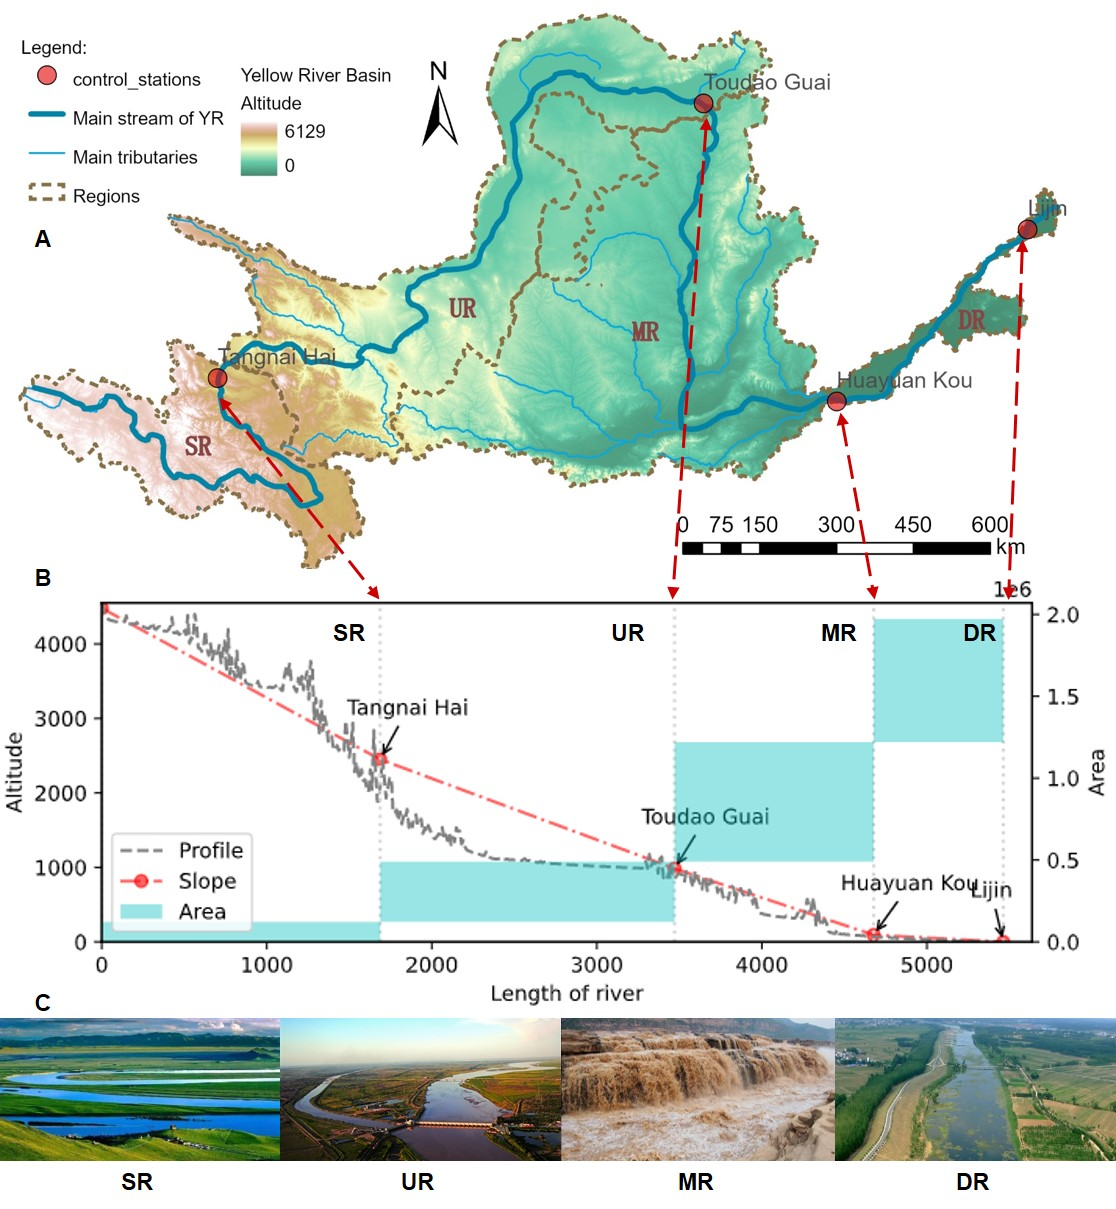
\includegraphics[width=\textwidth]{img/ch4/s1_study_area.jpg}
% \caption[黄河流域子区域划分]{黄河流域子区域划分。
%     \textbf{A.}黄河流域划分示意图(SR:源区,UR:上游,MR:中游,DR:下游);
%     \textbf{B.}黄河主河道剖面图,四个水文观测站分别控制SR、UR、MR和DR;
%     \textbf{C.}黄河流域不同地区的典型景观。}\label{fig:YRB}
% \end{figure}

\subsection{综合治理指数}

\subsubsection{综合指标构建方法}

% 将三者合一起,即:
如本章前文介绍以及框架图~\ref{ch4:fig:framework}所示,本研究定义的水资源治理综合指数(IWGI)应结合水治理的三个方面(``稀缺情况(S)''、``使用目的(P)''和``分配方式(A)'')。
由于每个指标维度都有升高和降低两个方向,在整合指标前应假设随着人类活动主导社会\textendash{}水文循环的进程,三者在其中某个方向对齐:
\begin{equation}
    Transformation \propto S*P*A
\end{equation}

接下来为三个方面选择了一个指标($I_x$, $x=S$, $P$,或$A$,分别对应``稀缺情况(S)''、``使用目的(P)''和``分配方式(A)'',来有效地量化这些方面,并将上式转化为自然对数,便于计算各指标对综合指数变化的贡献:
\begin{equation}
    Transformation \propto \ln(I_S) + \ln(I_P) + \ln(I_A)
\end{equation}
那么,综合水治理指数(IWGI)是标准化指标$I'_x$的平均值:
\begin{equation}
    IWGI = (I'_S + I'_P + I'_A) / 3
    \label{ch4:eq:IWGI}
\end{equation}
其中:
\begin{equation}
    I'_x = (I_x - I_{x, \min}) / (I_{x, \max} - I_{x, \min})
\end{equation}

对三个方面各自的指标选取如下文所述。

\subsubsection{子指标:水的稀缺情况}

水的``稀缺情况''既取决于气候能提供稀缺情况资源,还取决于灌溉和工业等经济活动的需求,更可以被水库蓄水、跨流域调水等工程所人为改变\cite{qin2019,wada2014,huang2021}。
本章研究采用Qin等人(2019)提出的稀缺性\textendash{}弹性\textendash{}易变性(SFV)水稀缺指数来评价``稀缺情况''的问题\cite{qin2019}。
这一指标考虑了管理措施(如水库的建设)和用水结构变化(有些用水方式如能源用水是难以被短期替代的),对水资源短缺情况做出评估。
此外,SFV指数从发展的角度关注水资源的动态,同时考虑了水资源的灵活性和易变性(例如气候差异带来的降水波动),是衡量水资源压力\cite{qin2019}时间变化的有效指标。
整个黄河流域的水分胁迫指标$I_S$为本章划分的四个二级区域$i$——源区(SR)、上区(UR)、中游(MR)、和下游(DR)指数$SFV_{i}$的平均值:

\begin{equation}
    I_S = \frac{1}{4} * \sum_{i=1}^4 SFV_{i}
    \label{ch4:eq:scarcity}
\end{equation}

其中$SFV_i$为区域$i$的SFV指数$SFV_i$,SFV结合了以下三个指标:

首先,对于稀缺性(Scarcity, S),$A_{i, j}$为区域$i$在第$j$年的耗水量占多年平均径流量的比例(本研究将为黄河流域划分为四个子区域,见\ref{ch4:sec:region}\nameref{ch4:sec:region}):

\begin{equation}
    A_{i, j} = \frac{WU_{i,j}}{R_{i, avg}}
\end{equation}

% TODO 完整的不灵活用水分类?
其次,对于灵活性(Flexibility, F),$F_{i, j}$是第$i$年和第$j$区域的不灵活用水$WU_{inflexible}$(例如能源行业冷却用水或人类和牲畜)占平均多年径流量的比例:

\begin{equation}
    F_{i, j} = \frac{WU_{i, j, inflexible}}{R_{i, avg}}
\end{equation}

最后,易变性(Variability, V)还考虑了水库容量和蓄水对自然径流波动的积极影响:
\begin{gather}
    C_i = C1_i * (1 - C2_i) \\
    C1_{i, j} = \frac{R_{i, std}}{R_{i, avg}} \\
    C2_{i} = \frac{RC_{i}}{R_{i, avg}}, \ if RC < R_{i, avg} \\
    C2_{i} = 1, \ if RC \geq  R_{i, avg}
\end{gather}

上式中,$R_{i, avg}$为$i$区域的平均径流量,$RC_i$为$i$区域水库的总库容,$R_{i, std}$为$i$区域径流量的标准差。

最后,该方法将三个指标(稀缺性S、灵活性F和易变性V)以相同的权重进行归一化后加权计算出$SFV$指标:

\begin{gather}
    V = \frac{A_{normalize} + B_{normalize} + C_{normalize}}{3}\\
    a = \frac{1}{V_{\max} - V_{\min}};\\
    b = \frac{1}{V_{\min} - V_{\max}} * V_{\min}\\
    SFV = a * V + b
\end{gather}


\subsubsection{子指标:水的使用目的}

水的``使用目的''与水能够提供的生态系统服务有关,但目前对文化、调节服务等缺乏成熟统一的评估框架,且受限于数据,本研究仅将用水分为供给用途(例如,日常饮用和食品生产)和非供给用途(例如能源冷却用水)的用水\cite{liu2017,florke2018,jaeger2019}。
本章研究使用供给服务目的在全部用水量中所占比例(Provisioning Purpose Shares, PPS)作为量化``使用目的(P)''$I_P$的指标。

\begin{equation}
    PPS = \frac{WU_{pro}}{WU_{pro} + WU_{non-pro}}
\label{ch4:eq:priority}
\end{equation}

其中($WU_{pro}$)为供给服务用水,包括家庭用水、灌溉用水和牲畜用水;非供给服务的用水($WU_{non-pro}$)包括工业用水和城市服务用水。
% 本章研究将牲畜用水、城乡生活用水和农业用水作为供应用水,因为它们直接服务于生存。其他的是非供应:服务和工业用水,因为它们主要为经济服务。

\subsubsection{子指标:水的分配方式}

最后,水的``分配方式''并非取决于区域的社会经济水平和自然环境背景,流域的水资源分配还会受到流域系统调度的工程(如水库统一调度)、非工程因素(如水资源分配制度)的影响\cite{schmandt2021,speed2013}。
本章借鉴使用熵作为刻画分配均匀程度的指标(式\ref{ch4:eq:allocation})\cite{peet1974},当不同区域间水资源使用完全平均时,当完全平均分配时该指标达到最大值$I_{A, \max} = 1$,当区域的用水量相差悬殊时$I_A \in [0, 1]$趋近于零。

\begin{equation}
    I_A = \sum_{i=1}^N - \log(p_{i}) * p_{i}
    \label{ch4:eq:allocation}
\end{equation}

其中$p_{i}$为区域$i$与整个流域的水量比例,由于本研究将黄河流域分为源区和上中下游,因此$N=4$。

\subsection{突变点检测}

本章研究采用Pettitt提出的的突变点检测方法,在不假设数据分布的情况下,对时间序列数据的单个变化点进行检测\cite{pettitt1979},它测试的原假设$H_0$是:变量不存在变化趋势差异,备择假设则为存在一个显著的趋势变化点。
通过将随机变量序列分为$\mathrm{x}_{1}, \mathrm{x}_{1}, \ldots, x_{t_{0}}$和$x_{t_{0}+1}, x_{t_{0}+2}, \ldots, x_{T}$表示的两段,如果每段都有一个共同的分布函数,即$F_1(x)$、$F_2(x)$和$F_1(x) \neq F_2(x)$,则在$t_0$处确定变化点。

为实现变化点的识别,定义统计指标$U_{t,T}$如下:

\begin{equation}
    U_{t, T} = \sum_{i=1}^t\sum_{j=t+1}^T sgn(X_i - X_j), 1 \leq t < T
\end{equation}

其中:
\begin{equation}
    \operatorname{sgn}(\theta)= \begin{cases}1 & \text { if } \theta>0 \\ 0 & \text { if } \theta=0 \\ -1 & \text { if } \theta<0\end{cases}
\end{equation}

找到最可能的变化点$\tau$,其值满足$K_{\tau} = \max|U_{t, T}|$,与值$K_{\tau}$相关的显著性概率近似计算为:

\begin{equation}
    p=2 \exp \left(\frac{-6 K_{\tau}^{2}}{T^{2}+T^{3}}\right)
\end{equation}

给定某个显著性水平$\alpha$,如果$p < \alpha$,则拒绝原假设并得出结论$x_{\tau}$是水平$\alpha$的显著突变点。

本章研究使用$\alpha = 0.001$作为显著性$p$的阈值,这意味着统计上显著的变化点判断有效的概率大于$99.9\%$。
迭代使用Pettitt算法:反复识别一个突变点从而将时间序列分为该时间点前后两段,并再次分别对两序列进行分析,直到检测到所有显著的突变点。
虽然接下来的结果展示的是阈值$\alpha = 0.001$的结果(识别出两个断点),但是经过敏感性分析,从$0.0005$到$0.05$的阈值范围选取都不影响本研究结果的鲁棒性(参见图\ref{ch4:fig:sensitivity})。

\begin{figure}[!ht] % use float package if you want it here
    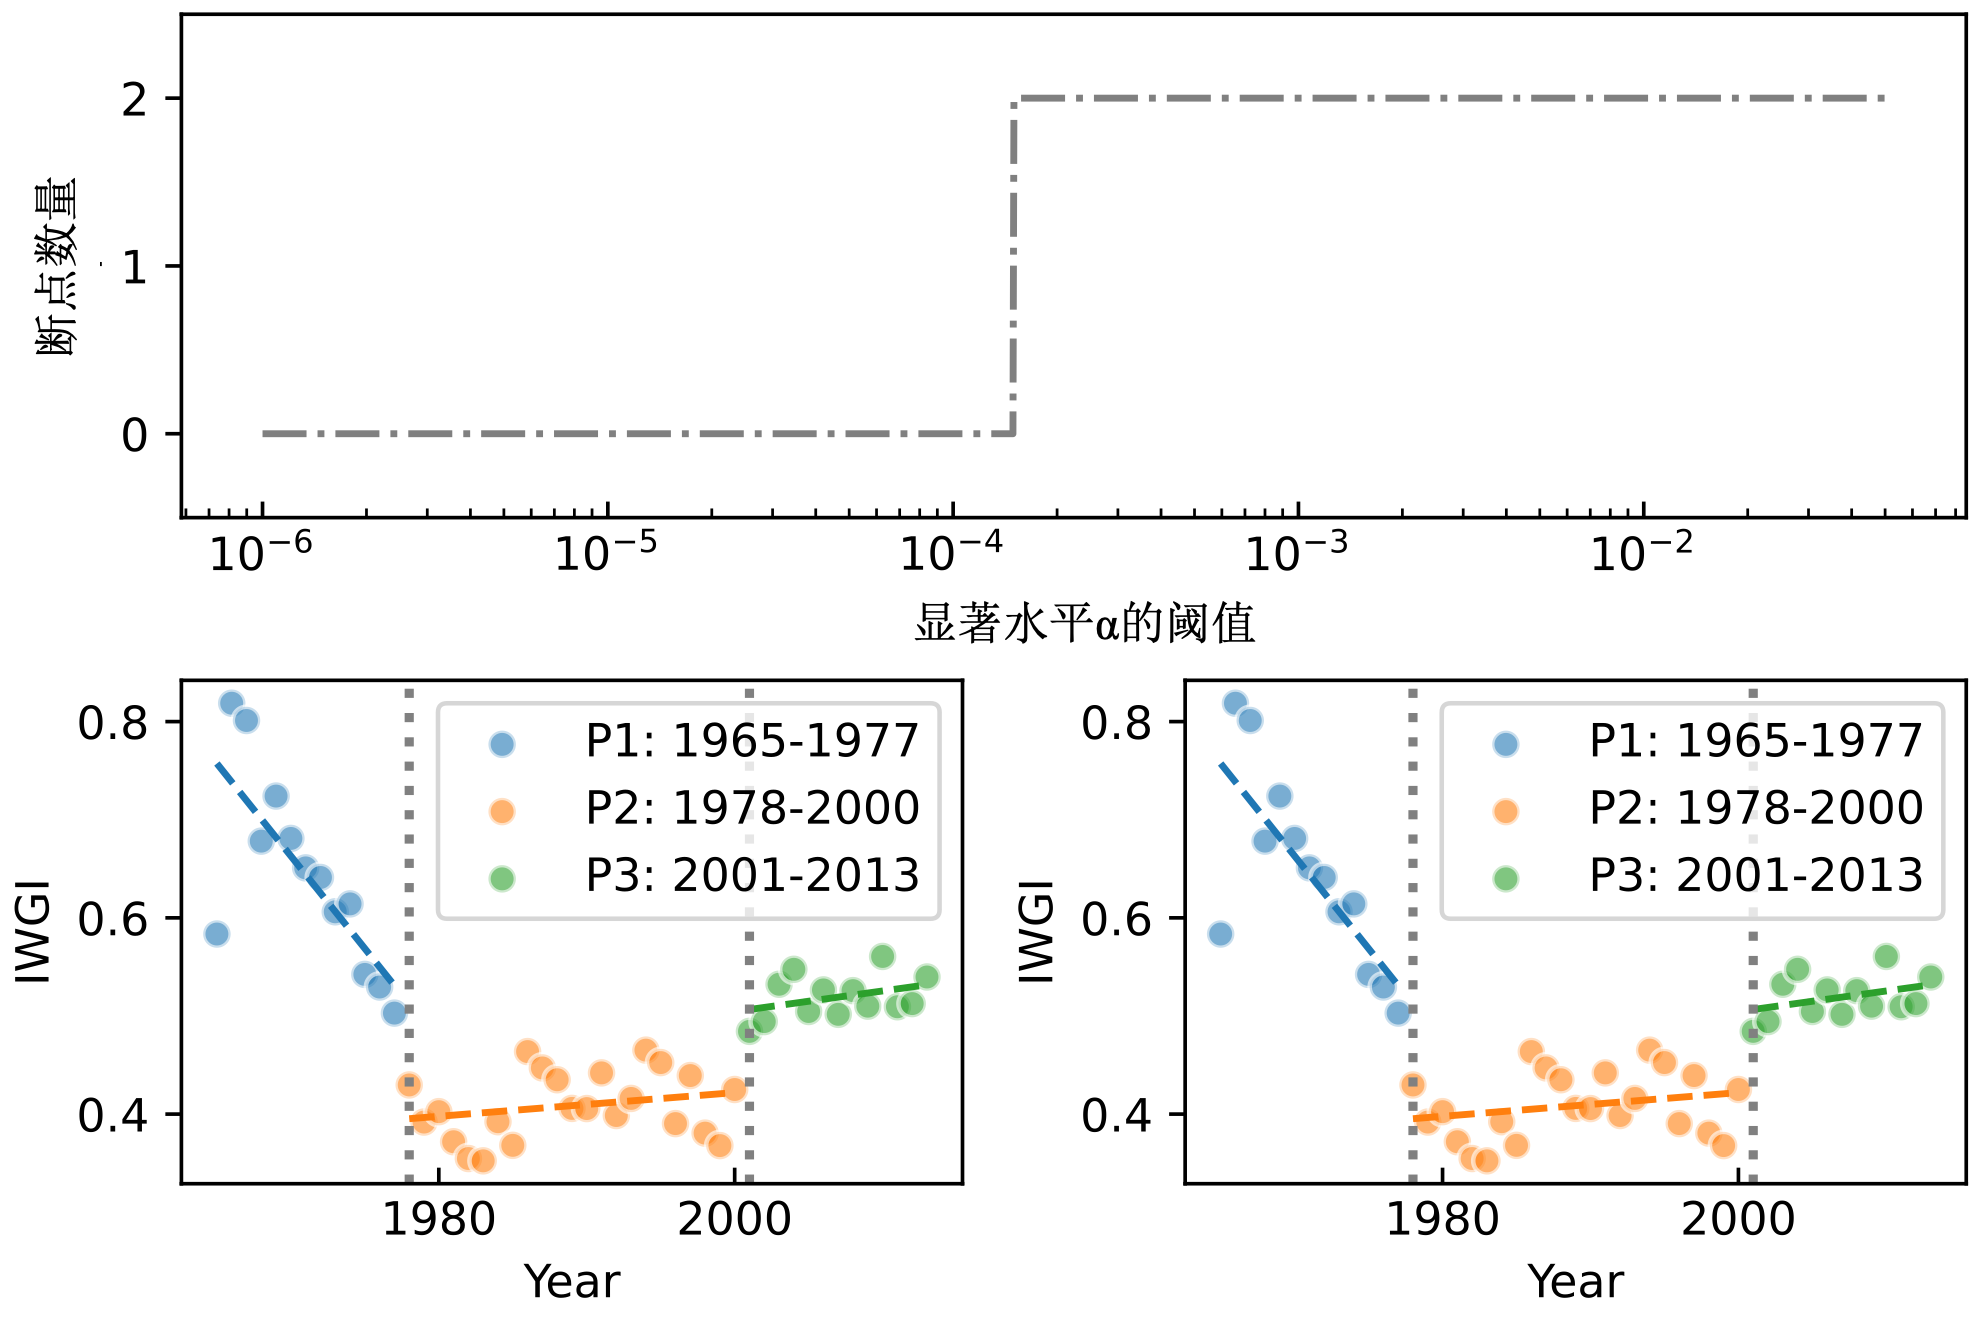
\includegraphics[width=\textwidth]{img/ch4/ch4_sensitivity.png}
    \caption[突变点检测中显著性阈值选取的敏感性测试]{突变点检测中显著性阈值选取的敏感性测试结果。
    \textbf{A} 选取不同阈值$\alpha$后识别的突变点个数,所有的方案都识别了两个断点。
    \textbf{B} 阈值选取为 $\alpha=0.0005$.
    \textbf{C} 阈值选取为 $\alpha=0.05$.}\label{ch4:fig:sensitivity}
\end{figure}

\subsection{数据来源}

% % Table generated by Excel2LaTeX from sheet '数据集'
\begin{table}[htbp]
    \centering
    \caption{数据分类与来源}
      \begin{tabularx}{\textwidth}{LLLLL}
      \toprule
      数据集   & 数据类型  & 空间尺度  & 时间尺度  & 数据来源 \\
      \midrule
      行政区水资源利用 & 统计    & 市级行政单元 & $1965-2013$ & Zhou等人2020 \\
      子流域水资源使用 & 统计    & 二级子流域 & $2003-2019$ & 水资源公报 \\
      GDP数据 & 统计    & 省级行政单元 & $1949-2019$ & 万德数据库 \\
      水库数据集 & 水文    & 站点数据  & $1949-2015$ & Wang等人2019 \\
      实测泾流量 & 水文    & 站点数据  & $1949-2019$ & Wang等人2019 \\
      黄河流域相关法律 & 文献    & 流域相关文件 & $1949-2013$ & 黄河流域规划 \\
      黄河水利委员会历史 & 文献    & 流域相关文件 & $1949-2002$ & 黄河水利委员会档案馆 \\
      黄河大事件 & 文献    & 流域相关文件 & $1949-2015$ & 黄河水利委员会档案馆 \\
      \bottomrule
      \end{tabularx}%
    \label{ch4:tab:data_source}%
\end{table}%
  

为了计算IWGI,使用了三个数据集:水库、实测径流、和用水。
水库数据集由Wang等人~\cite{wang2019c}收集,其中包括1956年以来新建的重要水库。
在所有水库中,黄河水利委员会已经将主要用于调节和管理的水库称为``主要水库''(见\url{http://www.yrcc.gov.cn/hhyl/sngc/})。
此外,每年的实测径流数据来自《黄河泥沙公报》(\url{http://www.yrcc.gov.cn/nishagonggao/}),分别由四个控制站(唐乃亥、头道拐、花园口、利津)在黄河的不同河段(源区、上游、中游、下游)进行测量得到。
水资源利用数据来源于Zhou等人\cite{zhou2020}发布的中国国家长期水资源利用数据集(NLWUD),包括地级市不同部门的用水量、用水经济变量和用水强度,我们以$95\%$相交面积为阈值筛选该数据集中的地级市,得到属于黄河流域的子数据集。

为了分析其变化的原因,灌溉面积、工业增加值和服务业总增加值以及用水强度数据也来自NLWUD数据集~\cite{zhou2020}。
此外,还使用了两个水治理政策数据集:法律政策和``大事件''文件数据集。
法律政策记录(表~\ref{ch4:tab:policies})来源于2013年公开批准的``黄河流域综合规划'',其中回顾了建国以来全流域尺度上的重要法律法规。
与黄河有关的``大事件''的原始文件则来自黄河水利委员会的记录和汇编(\url{http://www.yrcc.gov.cn/hhyl/hhjs/})。

本研究中使用或分析的所有数据,包括水库数据集、测量径流、用水数据集、规律和大事件,都已储存在公开获取的数据仓库中(\url{https://doi.org/10.5281/zenodo.7955500}~\cite{shuang_song_2023_7955500})。

% Table generated by Excel2LaTeX from sheet '黄河流域法律政策'
\begin{table}[htbp]
    \centering
    \caption{黄河流域法律政策}
      \begin{tabularx}{\textwidth}{L p{1.5cm} L}
      \toprule
      法律或政策名称 & \multicolumn{1}{l}{施行或修订时间} & 颁布机构 \\
      \midrule
      中华人民共和国水法 & 1,988 & 全国人民代表大会常务委员会 \\
      中华人民共和国水法  修正 & 2,002 & 全国人民代表大会常务委员会 \\
      中华人民共和国水法  第一次修订 & 2,009 & 全国人民代表大会常务委员会 \\
      中华人民共和国水法  第二次修订 & 2,016 & 全国人民代表大会常务委员会 \\
      中华人民共和国水污染防治法 & 1,984 & 全国人民代表大会常务委员会 \\
      中华人民共和国水污染防治法  修正 & 1,996 & 全国人民代表大会常务委员会 \\
      中华人民共和国水污染防治法  第一次修订 & 2,008 & 全国人民代表大会常务委员会 \\
      中华人民共和国水污染防治法  第二次修订 & 2,018 & 全国人民代表大会常务委员会 \\
      取水许可和水资源费征收管理条例 & 2,006 & 中华人民共和国国务院 \\
      取水许可和水资源费征收管理条例  第一次修订 & 2,017 & 中华人民共和国国务院 \\
      黄河水量调度条例 & 2,006 & 中华人民共和国国务院 \\
      黄河可供水量分配方案 & 1,987 & 中华人民共和国国务院 \\
      取水许可管理办法 & 2,008 & 中华人民共和国水利部 \\
      取水许可管理办法  第一次修订 & 2,015 & 中华人民共和国水利部 \\
      取水许可管理办法  第二次修订 & 2,017 & 中华人民共和国水利部 \\
      黄河水量调度条例 & 2,006 & 中华人民共和国国务院 \\
      黄河可供水量年度分配及干流水量调度方案 & 1,998 & 国家发展计划委员会,水利部 \\
      黄河水量调度管理办法 & 1,998 & 国家发展计划委员会,水利部 \\
      黄河水权转换管理实施办法 & 2,004 & 水利部 \\
      取水许可和水资源费征收管理条例 & 2,006 & 中华人民共和国国务院 \\
      取水许可证制度实施办法 & 1,993 & 中华人民共和国国务院 \\
      建设项目水资源论证管理办法 & 2,002 & 国家发展计划委员会,水利部 \\
      水利工程管理体制改革实施意见 & 2,006 & 中华人民共和国国务院 \\
      \bottomrule
      \end{tabularx}%
    \label{ch4:tab:policies}%
  \end{table}%
  

\subsection{数据分析}

\subsubsection{相关分析与显著性检验}

皮尔逊相关系数(Pearson correlation coefficient,通常用 $r$ 表示)是用于衡量两个连续变量之间线性关系强度的指标。它的值范围在 $-1$ 到 $1$ 之间,其中 $-1$ 表示完全负相关,$1$ 表示完全正相关,$0$ 表示无相关性,本研究使用该指标反映某时段内IWGI的趋势同哪些子指标变化趋势更密切,为了计算两个变量之间的皮尔逊相关系数,我们可以使用以下公式\cite{freedman2007}:

\begin{equation}
    r = \frac{\sum_{i=1}^{n}(x_i - \bar{x})(y_i - \bar{y})}{\sqrt{\sum_{i=1}^{n}{(x_i - \bar{x})}^2}\sqrt{\sum_{i=1}^{n}{(y_i - \bar{y})}^2}}
\end{equation}

其中,$x_i$ 和 $y_i$ 分别表示第 $i$ 个观察值,$\bar{x}$ 和 $\bar{y}$ 分别表示 $x$ 和 $y$ 的均值,$n$ 表示观察值的数量。计算出皮尔逊相关系数后,我们需要进行显著性检验来确定这种关系是否具有统计显著性。这里我们使用 $t$ 检验来计算显著性水平。根据 $r$ 和样本大小,我们可以计算 $t$ 值\cite{freedman2007}:

\begin{equation}
    t = \frac{r\sqrt{n-2}}{\sqrt{1-r^2}}
\end{equation}

根据统计量$t$的值查表判断显著性水平,如果 $p$ 值低于预先设定的显著性水平$0.01$,则我们可以认为两个变量之间的关系具有统计显著性。在实际应用中,我们使用 scipy 1.10.1~\cite{2020SciPy-NMeth}完成这些计算。

\subsubsection{基于平均的指标贡献度}

本研究中,表征稀缺情况的SFV指数就是稀缺性(S)、弹性(F)、易变性(V)三个指标在不同区域(源区、上游、中游、下游)之间的等权重平均(见式\ref{ch4:eq:scarcity}),综合水治理指标(IWGI)则是稀缺情况、使用目的、分配方式三个子指标取对数后的等权重平均(见式\ref{ch4:eq:IWGI})。
对此类指数,本研究中使用如下方法计算某时段某子指标($X$)对总指标变化(或指标/地区均值)的贡献度$Contribution_{X}$:

\begin{equation}
    Contribution_{X} = \Delta_{X} / \Delta_{Index}
\end{equation}

其中$\Delta_{X}$是该子指标在给定时段(从$t=start$到$t=end$)内的总变化值,$\Delta_{I}$是该子指标参与贡献的总指标总变化,两者都可以使用如下公式计算:

\begin{equation}
    \Delta=\sum_{t=start}^{end}(X_{t}-X_{t-1})
\end{equation}

上述计算方法可以计算不同时间段、不同指标的贡献度,帮助了解各指标在特定时间段内对总体变化的影响程度。

\subsubsection{基于比例的指标贡献度}

本研究中供给性用水比例(表征使用目的,见式\ref{ch4:eq:priority})以除法形式进行计算,在分解各部门用水对比例变化的贡献时应取对数:

\begin{equation}
    \log{(\text{ratio})}=\log{\frac{A}{B}} = \log{A} - \log{B}
    \label{ch4:eq:log}
\end{equation}

本章感兴趣的是在时段开始($start$)到结束($end$)之间 $C$、$A$ 和 $B$ 的变化,我们可以将 C 的变化量表示为 A 和 B 变化量的加权和:

\begin{equation}
    \begin{aligned}
    & \Delta \log (C)=\log \left(C_{end}\right)-\log \left(C_{start}\right) \\
    & \Delta \log (A)=\log \left(A_{end}\right)-\log \left(A_{start}\right) \\
    & \Delta \log (B)=\log \left(B_{end}\right)-\log \left(B_{start}\right) \\
    & \Delta \log (C)=k_1 \cdot \Delta \log (A)+k_2 \cdot \Delta \log (B)
    \end{aligned}
\end{equation}

结合式\ref{ch4:eq:log},可以得到A 和 B 分别对 C 变化的贡献比例 $k_1$ 和 $k_2$:

\begin{equation}
    \begin{gathered}
    k_1=\frac{\Delta \log (C)}{\Delta \log (A)} \\
    k_2=\frac{\Delta \log (C)-\Delta \log (A)}{-\Delta \log (B)}
    \end{gathered}
\end{equation}


\section{人类活动主导时期人水关系演变过程}\label{ch4:process}
\subsection{综合指标变化过程}\label{ch4:sec:process}

\begin{figure*}[ht!]
	\centering
	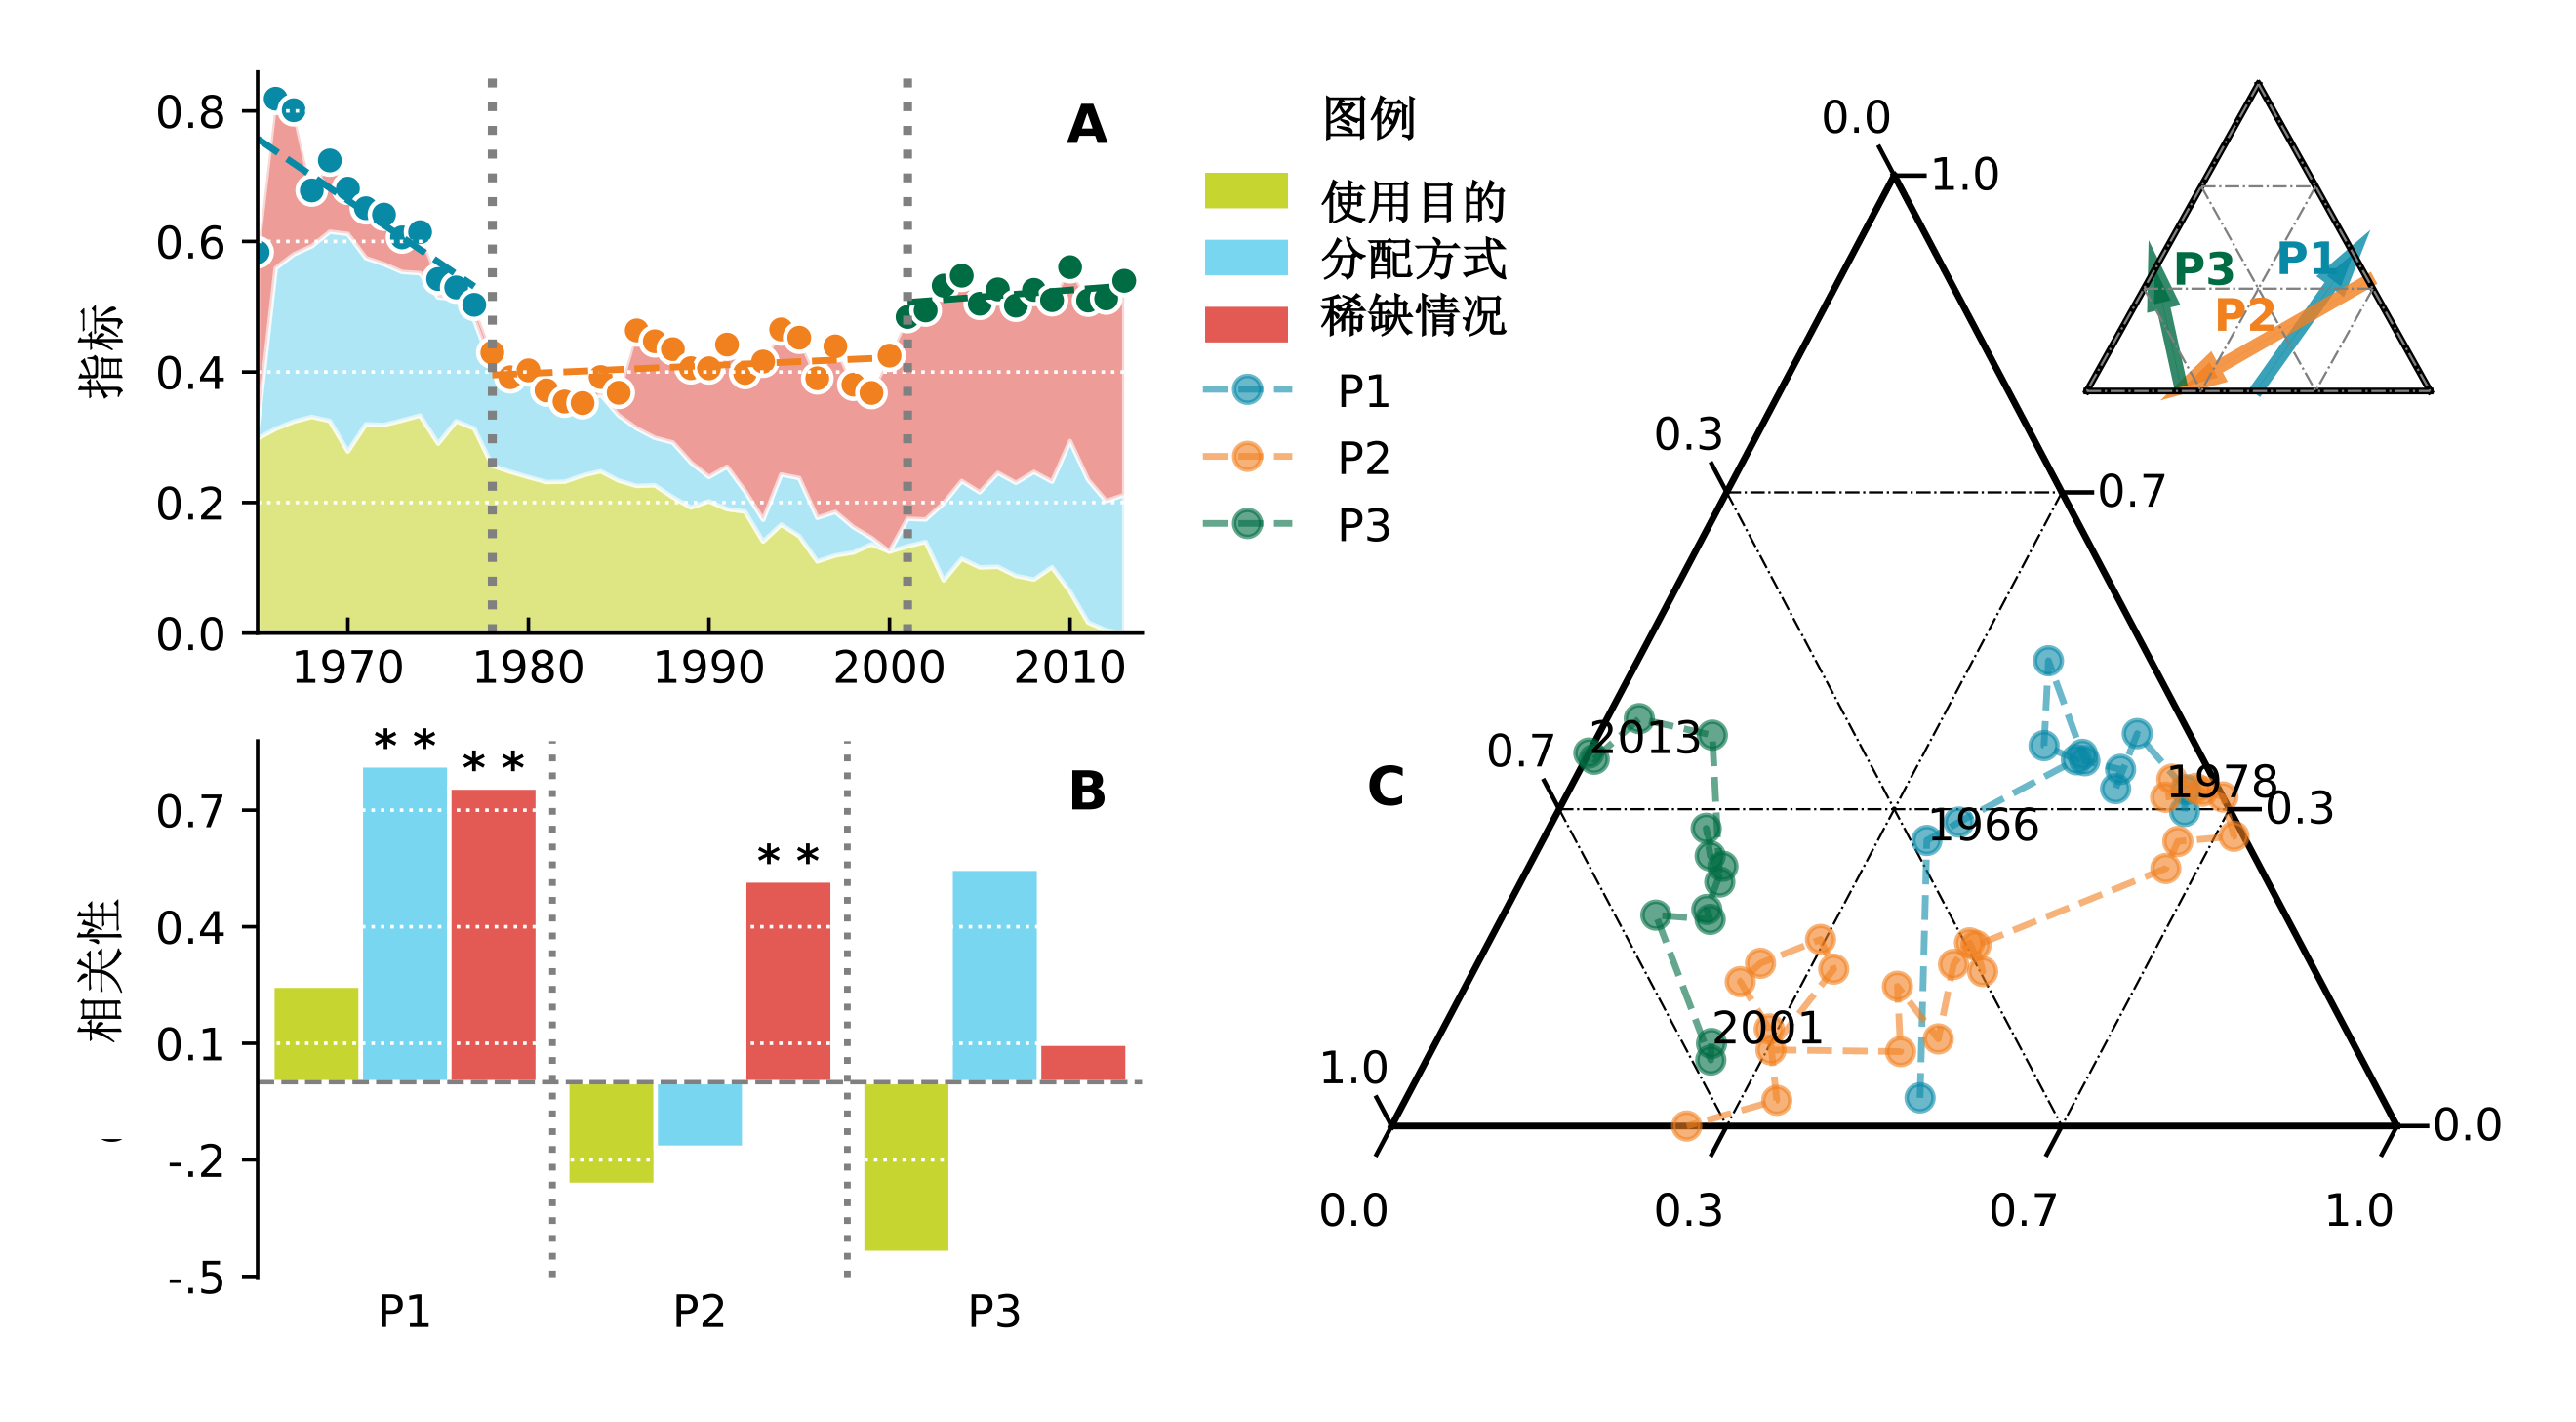
\includegraphics[width=\textwidth]{img/ch4/ch4_index.png}
	\caption[IWGI指数反映黄河流域的水治理变化阶段]{IWGI指数反映黄河流域的水治理变化阶段。两个突变点将1965年以来的黄河流域水治理划分为三个阶段,第一阶段(P1): $1965 \sim 1978$,第二阶段(P2): $1979 \sim 2001$,第三阶段(P3): $2002 \sim 2013$。
	\textbf{A,} 检测IWGI的突变点和三个指标的各自贡献:“稀缺情况(S)”、“使用目的(P)”和“分配方式(A)”。1978年和2001年出现了两个显著的变化点($p<0.01$)。
	\textbf{B,}  各阶段的IWGI变化与三个指标各自变化的相关性。
	\textbf{C,} IWGI随时间变化的同时,三个指标贡献比例的组合不断改变,致使水治理向不同方向发生阶段性转移。
	}\label{ch4:fig:IWGI}
\end{figure*}

IWGI在研究时段内存在两个突变点,将1965年以来的黄河流域水治理划分为三个阶段,第一阶段(P1): $1965 \sim 1978$,第二阶段(P2): $1979 \sim 2001$,第三阶段(P3): $2002 \sim 2013$,而“稀缺情况(S)”、“使用目的(P)”和“分配方式(A)”的三个指标在每个阶段的贡献不同(图~\ref{ch4:fig:IWGI}A)。
% 第一阶段
在第一个时期(P1, $1965 \sim 1978$)水资源压力对IWGI的贡献很小,“使用目的”和“分配方式”的指标的贡献更大(平均分别为$49.45\%$和$34.95\%$),但均呈现出显著的下降趋势($p<0.01$,图~\ref{ch4:fig:IWGI}~B),导致此时期IWGI迅速下降。
% 第二阶段
在第二阶段(P2, $1979 \sim 2001$),水资源压力指标的显著增加($p<0.01$)并为IWGI的略微上升做出主要贡献($p<0.01$,图~\ref{ch4:fig:IWGI}~A),而“使用目的”和“分配方式”的指标对IWGI的变化起了消极作用。
% 第三阶段
最后,在第三个时期(P3, $1995 \sim 2013$),尽管水资源压力指标在贡献中保持着$57.11\%$的最突出份额,但其数值已几乎保持不变,反而是“使用目的”的指标的降低和“分配方式”指标的增加,共同推动了综合指标IWGI的变化。
%的整体
综上所述,“稀缺情况(S)”、“使用目的(P)”和“分配方式(A)”的三个指标在不同时期对黄河流域水治理整体特征变化的贡献不同,将其演变历史划分为明显的三个阶段,依据其各自特点可命名为:集中供水时期、治理转变时期、适应增强时期(对应时间阶段分别为$1965 \sim 1978$、$1979 \sim 2001$、$2002 \sim 2013$(图~\ref{ch4:fig:IWGI}~C)。

\subsection{稀缺情况指标变化}

构成稀缺情况的指标(SFV指数)在研究时段(包括三个不同时期)内呈现出先降低、然后迅速增加、最后再次略微降低的变化趋势(图~\ref{ch4:fig:scarcity}~A)。
% ,表明水资源压力先减少再迅速增加,后趋于稳定
源区、上游、中游、下游这四个不同的区域中(图~\ref{ch4:fig:scarcity}~B),源区对三个时段的SFV指标变化几乎没有贡献,下游也仅在治理转变时期和适应增强时期呈现微弱的负向贡献。
对稀缺情况影响最大的是黄河的上游和中游,上游在集中供水时期和治理转变时期都是SFV变化的最大贡献区域,中游则在适应增强时期做出最大贡献。

\begin{figure}[!ht]
  \centering
  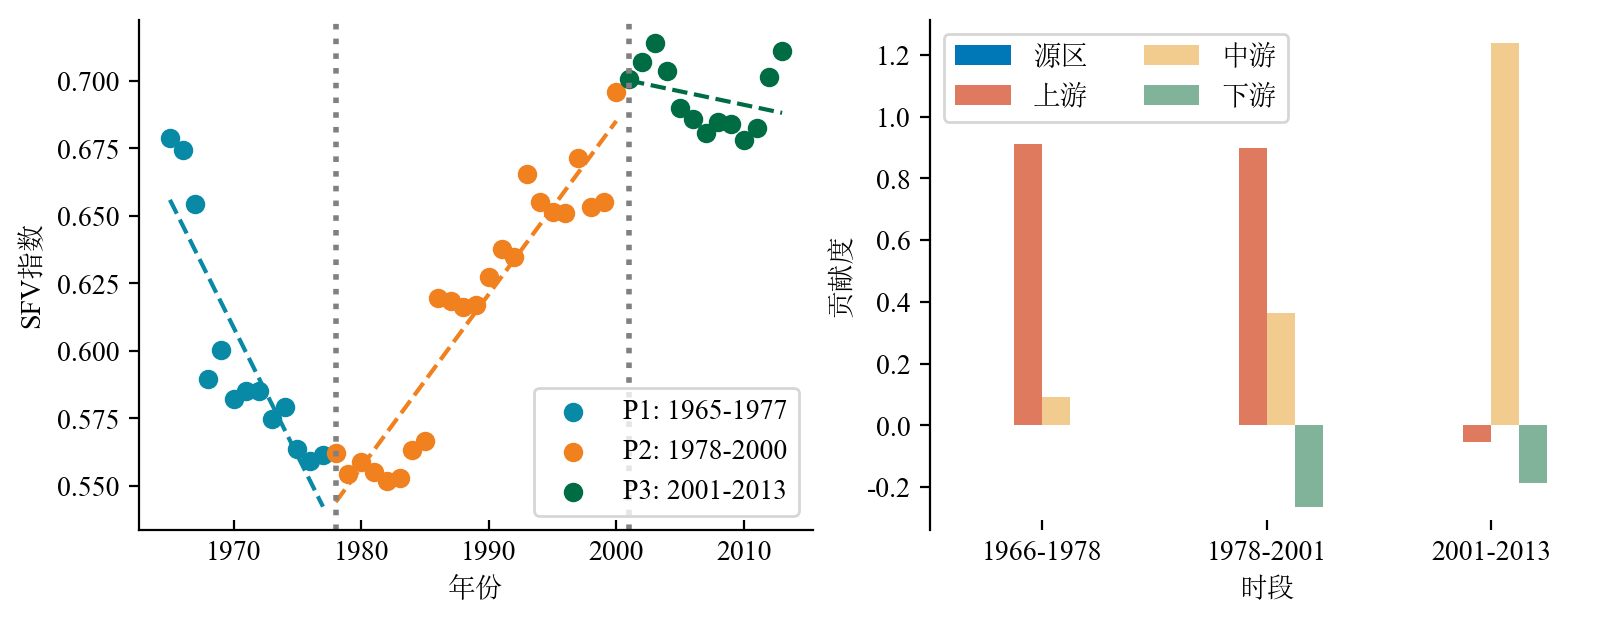
\includegraphics[width=\textwidth]{img/ch4/ch4_scarcity.png}
  \caption{稀缺性SFV指标变化趋势及各区域贡献}\label{ch4:fig:scarcity}
\end{figure}


\subsection{使用目的指标变化}

在用水目的上,供给性用水比例在集中供水时期基本保持不变,但在治理转变时期和适应增强时期呈现迅速下降的趋势(图\ref{ch4:fig:priority}~A)。
三个时段都是由灌溉用水的变化主导了该比例变化,城市、农村的人居用水、农村牲畜用水等几乎对该比例的变化没有影响(图\ref{ch4:fig:allocation}~B)。

\begin{figure}[!ht]
	\centering
	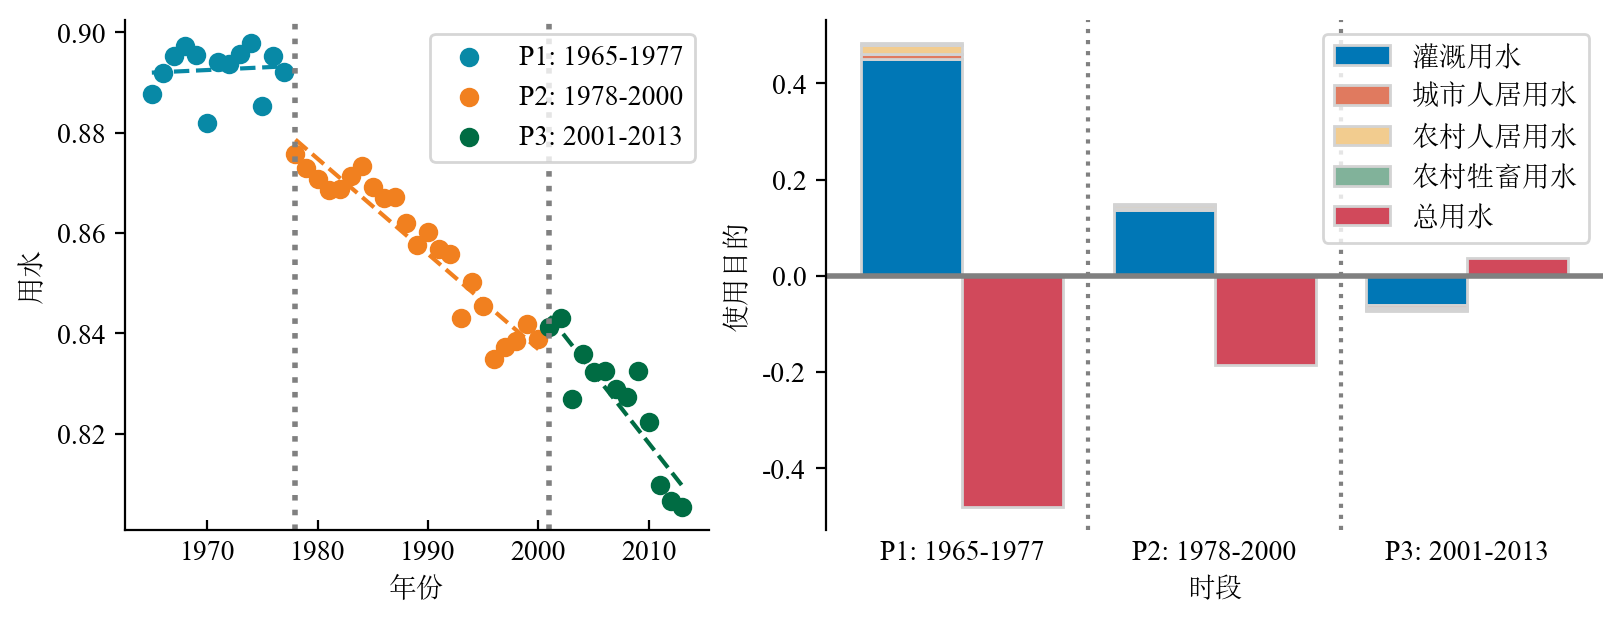
\includegraphics[width=\textwidth]{img/ch4/ch4_priority.png}
	\caption{供给性用水所占比例的变化趋势及各部门贡献}\label{ch4:fig:priority}
\end{figure}

\subsection{分配方式指标变化}

分配方式的指标变化呈现明显“V形”趋势,表明黄河的源区、上游、中游、下游之间水资源呈现先逐渐远离均匀分配,又在2000年后逐渐趋于平均的变化过程(图\ref{ch4:fig:allocation})。

\begin{figure}[!ht]
	\centering
	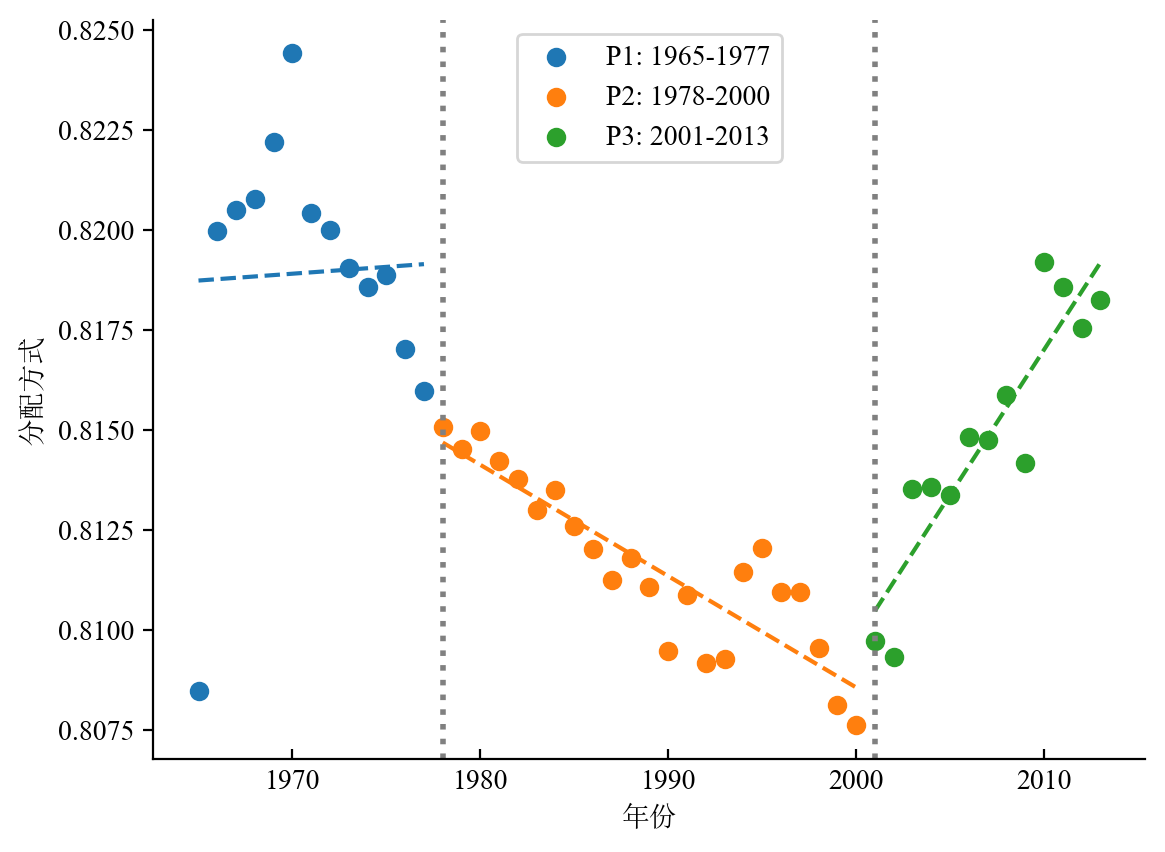
\includegraphics[width=0.6\textwidth]{img/ch4/ch4_allocation.png}
	\caption{分配方式指标的变化趋势}\label{ch4:fig:allocation}
\end{figure}

\section{人类活动主导时期人水关系演变机制}\label{ch4:mechanism}

% \subsection{水治理变化的驱动力分析}\label{ch4:sec:mechanism}

\begin{figure}[th!]
	\centering
	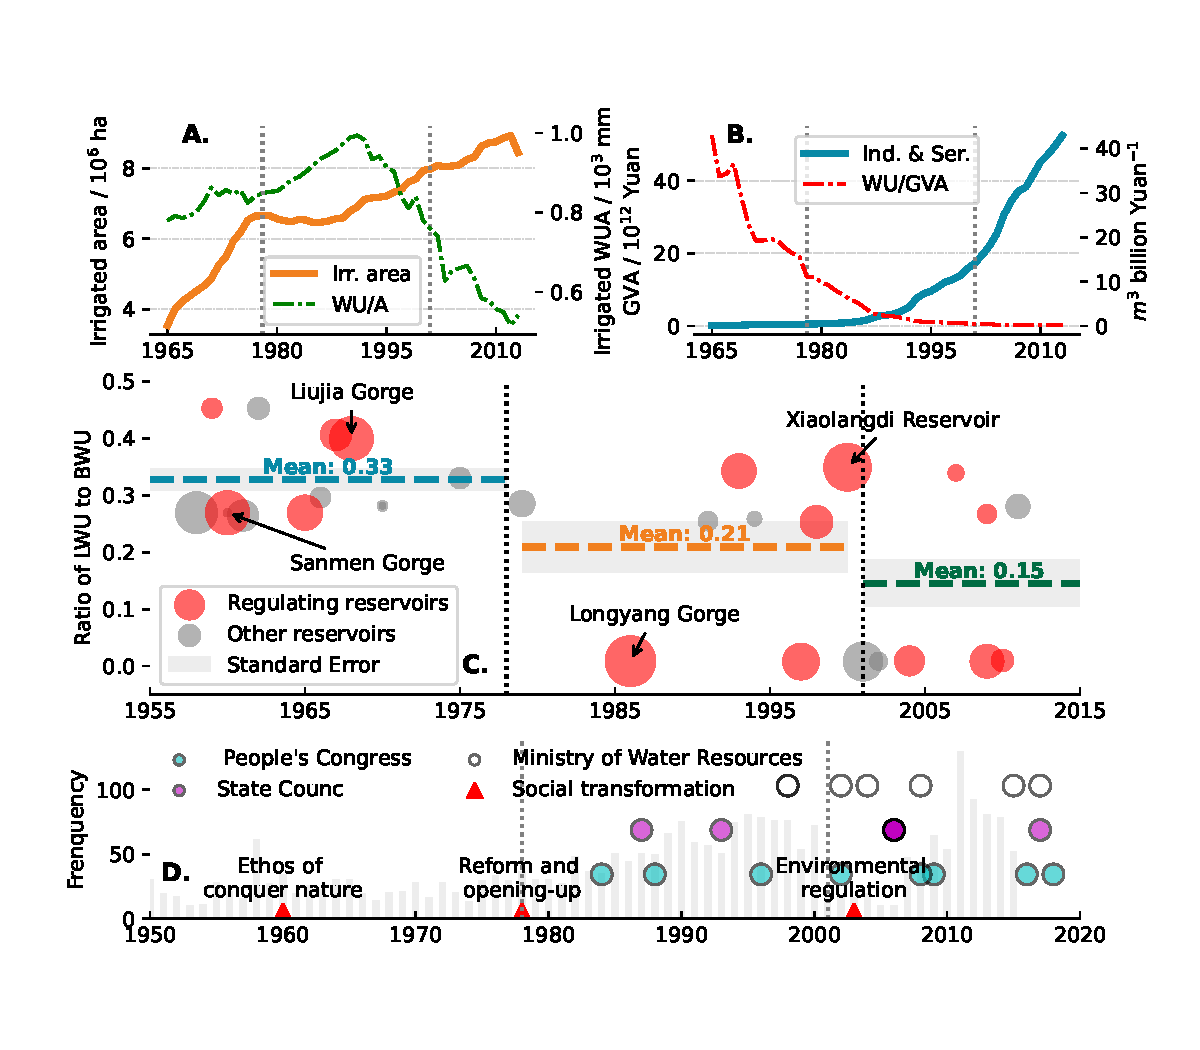
\includegraphics[width=\textwidth]{img/ch4/causes.pdf}
	\caption[黄河流域水治理阶段变化的驱动因素]{
		黄河流域水治理阶段变化的驱动因素。
		\textbf{A.}总灌溉面积($A$, 橙色线)和用水强度($WU/A$,用水量除以灌溉面积,绿点线)的变化。
        \textbf{B.}工业和服务业的总增加值(蓝线,$GVA$)变化及其用水强度($WU/GVA$,WU除以GVA,红点线)。
        \textbf{C.}每个水库的完工时间及其所在区域的用水量(Local Water Use, LWU)占水库完工时流域总用水量(Basinal Water Use, BWU)的百分比。红圈为负责黄河流域综合调度的水库。每个圆圈的大小表示其储水能力的大小。
        \textbf{D.}社会转型(红色三角形)和国家层面的治理政策(圆圈,不同颜色表示由不同的国家机构签署,越靠上代表国家机构的登记越高,详见表\ref{ch4:tab:policies})。浅灰色条形图以流域尺度(黄河大事件)计算与黄河流域有关的官方治理文献记录。}\label{ch4:fig:mechanism}
\end{figure}


\begin{figure}[tb]
    \centering
    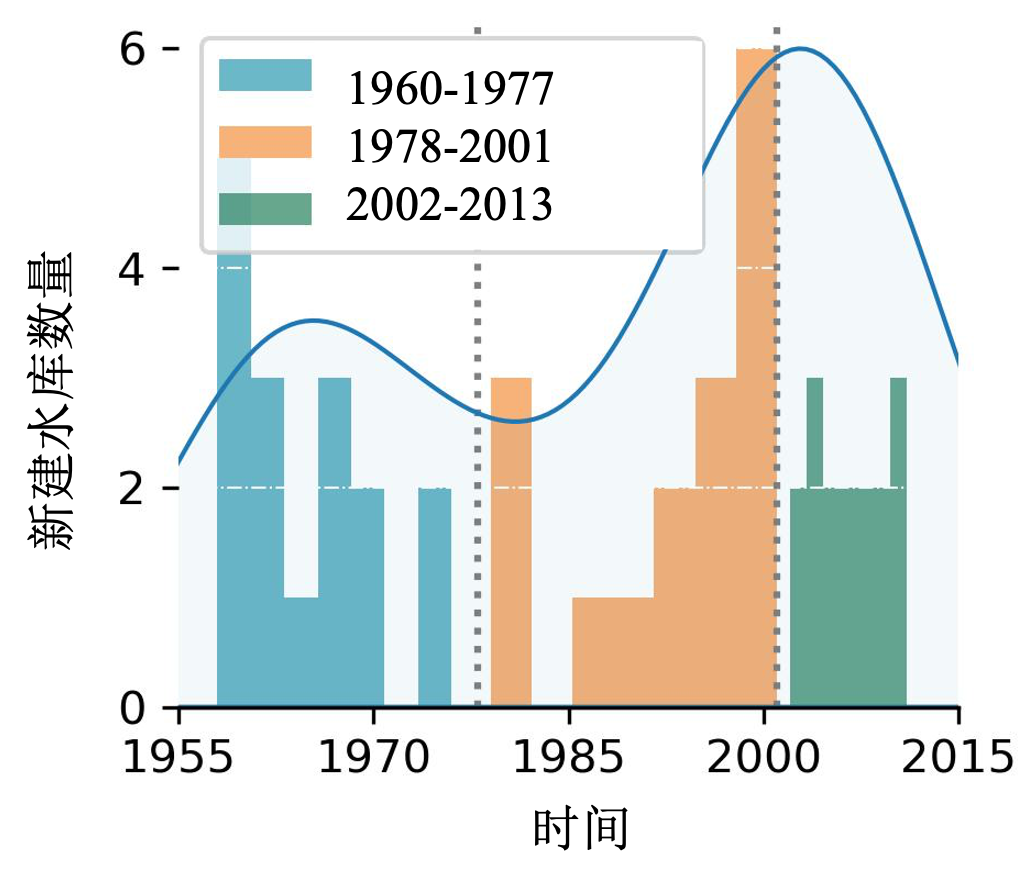
\includegraphics[width=0.6\linewidth]{img/ch4/ch4_reservoirs.png}
    \caption{黄河流域新增水库数量的时间分布}\label{ch4:fig:reservoirs}
\end{figure}


本节进一步探讨了致使IWGI变化的原因,灌溉区扩张和工业和服务业的经济增长是推动“集中供水时期”和“治理转变时期”两个阶段变化的关键。
黄河流域的用水需求在“集中供水时期”迅速增加,尤其是灌溉农业面积以$0.25*10^6 ha/yr$的速度迅速扩张(图\ref{ch4:fig:mechanism}~A),同时通过建设水库增加供应(图~\ref{ch4:fig:reservoirs})。
进入“治理转变时期”后,尽管灌溉区扩张停滞,但工业和服务业的发展开始增长,共同推动流域用水需求的进一步增加(图\ref{ch4:fig:mechanism}~A和B)。
接下来从“治理转变时期”到“适应增强时期”的演变过程中,水分利用效率变化最明显。
在“适应增强时期”,不仅工业和城市服务也承担了更重要的经济角色(由总增加值GVA表示,图\ref{ch4:fig:mechanism}~B),灌溉面积也恢复了缓慢扩张(图\ref{ch4:fig:mechanism}~A)。
但因用水效率的普遍提高,单位灌溉面积或单位产量的用水量都显著下降(图~\ref{ch4:fig:mechanism}~A和图~\ref{ch4:fig:mechanism}~B),因此部门和地区之间的用水差异在不断缩小,但流域水资源压力总体、持续维持在较高水平,公平合理分配宝贵水资源的压力越来越大(图~\ref{ch4:fig:IWGI}~A)。

最后,环境背景、社会文化、水治理政策等因素为三个时期的指标变化都产生了影响。
本研究首先计算了每个水库的区域用水量和流域用水量之比,较高的比值代表了该水库等潜在作用更有可能是旨在为该流域供水而不是流域调度;此外,流域调度的枢纽水库也以红色进行了标记(图~\ref{ch4:fig:mechanism}~C)。
可以看到,在阶段一的“集中供水时期”,受“人定胜天”的社会环境引领,大部分水库都建在需水量较大的地区,因此区域用水量和流域用水量之比值明显较高($p<0.01$,见图~\ref{ch4:fig:mechanism}~C)。
进入“治理转变时期”之后,新建水库的数量明显减少且多为枢纽水库,但全流域层次的法律法规(包括著名的“八七”分水方案)开始被不断提出,流域内的治理记录也迅速增加,可见此时期层出不穷的流域政策已深刻影响了流域水治理,流域水治理正在进行一场从工程措施向非工程措施的“治理转变”(图~\ref{ch4:fig:mechanism}~D, $p<0.01$和图\ref{ch4:fig:reservoirs})。
最后在“适应增强时期”,持续高位的水压力已成为制约区域发展的瓶颈,亟需通过节水转型和跨区域协调、调水来满足经济发展的用水需求,因此并且“大规模进行环境治理和节水转型”的国家战略指导下,有关部门提出了更多的、级别更高的水治理决策(图~\ref{ch4:fig:mechanism}~D)。
综上所述,从“集中供水时期”到“治理转变时期”的转变与当时水资源供需的增加相一致;而“治理转变时期”到“适应增强时期”的演变过程则是在水资源压力趋于稳定的同时,由社会监管政策和节水转型带来的效率提高所驱动的。

\section{讨论}\label{ch4:discussion}
\section{流域水治理演变模式}

研究结果显示黄河流域在人类主导时期有三种不同的流域治理模式:集中供水时期(P1: $1965 \sim 1978$)、治理转变时期(P2: $1979 \sim 2001$)和适应转向时期(P3: $2002 \sim 2013$)(图~\ref{ch4:fig:IWGI})。
在黄河流域水资源压力相对较低的集中供水时期($1965 \sim 1978$年),主要的水资源需求是为牲畜和作物等供给服务为目的,水治理也倾向于通过建造水库和引水渠等来增加水资源供给。
然而,正如当时“人定胜天”的口号所暗示的那样,水资源供应的增加并不能促进人-水关系和谐,因为它在不考虑生态保护的情况下急剧增加了用水,且这常常是一种不可逆转的变化\cite{zhou2020}。
在接下来的十年内,灌溉农田和引水设施的迅速扩张使黄河流域超负荷取水,在1972年以来,超过$80\%$的地表水被使用,导致河流频繁枯竭,造成了额外的生态问题,如湿地萎缩和生物多样性下降\cite{wang2019c}。
此外,由于水资源压力也限制了新兴的、更有利可图的工业与服务业的发展,这让流域的水治理模式接近了社会-生态危机的临界点,因为继续增加供应无论如何都是不切实际的\cite{loch2020, wohlfart2016a}。

治理体制转型时期的开始(P2: $1979 \sim 2001$)恰逢“改革开放”后,水资源竞争的持续加剧,但枯竭的黄河已经开始断流。
黄河流域在此时期开始水治理转变,这一结果与理论分析的结果高度一致:在流域总供应稳定的情况下,水资源需求在接近可供给水资源上限后的持续增长,将为流域水治理带来重大转型,流域社会-水文系统将通过制度措施让快速增强社会适应力,以响应该水资源供小于求的临界点\cite{loch2020}。
因此黄河流域在此时期发起了诸多水治理举措,包括控制灌溉面积的增长、倡导节水设施建设、制定全国首个水资源配额制度、并初步制定跨流域调水方案(南水北调)等\cite{wang2019b,long2020,nickum2021},成为了中国九大流域的制度变革先驱。
因此,尽管黄河流域的水资源压力仍然很大,且因径流减少和用水灵活性降低而持续增加,但黄河的断流问题却得到了解决,$1999$年的最后一次断流向世人昭示着此次水治理转变的巨大影响\cite{wang2019b}。

在随后的适应增强时期(P3: $2002 \sim 2013$)为适应稳定在高位的水资源压力,许多国家层面的黄河流域水治理实践都在这一时期提出,以期用最经济地方式,在保护生态的同时实现流域高质量发展。
二十一世纪初提出的“环境整治”和$2011$年提出的“最严格水资源管理”都是对水资源粗放式开发利用的响应,不断使流域水治理模式变得更高效。
这一时期除了中央政府主导的适应举措,地区各部门之间为了追求生产效率,社会经济过程为“水怎么用、水怎么分”的权衡发挥了重要作用。
典型的例子是黄河流域的水权转换工作,许多地区都积极推动了农业节水转型,并将节约的水额供给到经济效益更高的工业服务业之中。
通过不同行业和地区对流域水资源的广泛重建,通过日益强化的社会-经济过程调整以前粗放的发展模式以及刚性的制度约束,这些都是水治理适应性增强的体现,才能在有限的供水条件下优化平衡来自不同地区、不同行业的需求\cite{dalin2015,song2022}

黄河流域的水治理演化过程是“增大供给、治理转变、适应增强”的突出的案例,而其中变化的内在机制已在世界人类主导流域社会-水循环的过程中广泛出现(图~\ref{fig:summary})。
随着社会-经济过程对水循环影响加深,不同时期的流域面临不同的水治理挑战:在前期主要是经济和环境方面,在后期集中于与制度和政策方面。
放眼全球其它流域,以水资源短缺和供水困难为代表的水治理挑战是制约发展中流域的瓶颈\cite{allan2019,speed2013,liu2012a}。
人类社会-经济过程主导的发达流域(特别是跨界河流)则须重点解决结构性挑战,如水纠纷或缺乏公平\cite{mirumachi2015}。
本章研究开发并使用的综合水治理指数(IWGI)可以将流域水治理变化过程与这些挑战联系起来,提供了一种解释人类活动主导下人-水关系变化的方法。

\begin{figure}[htbp!]
	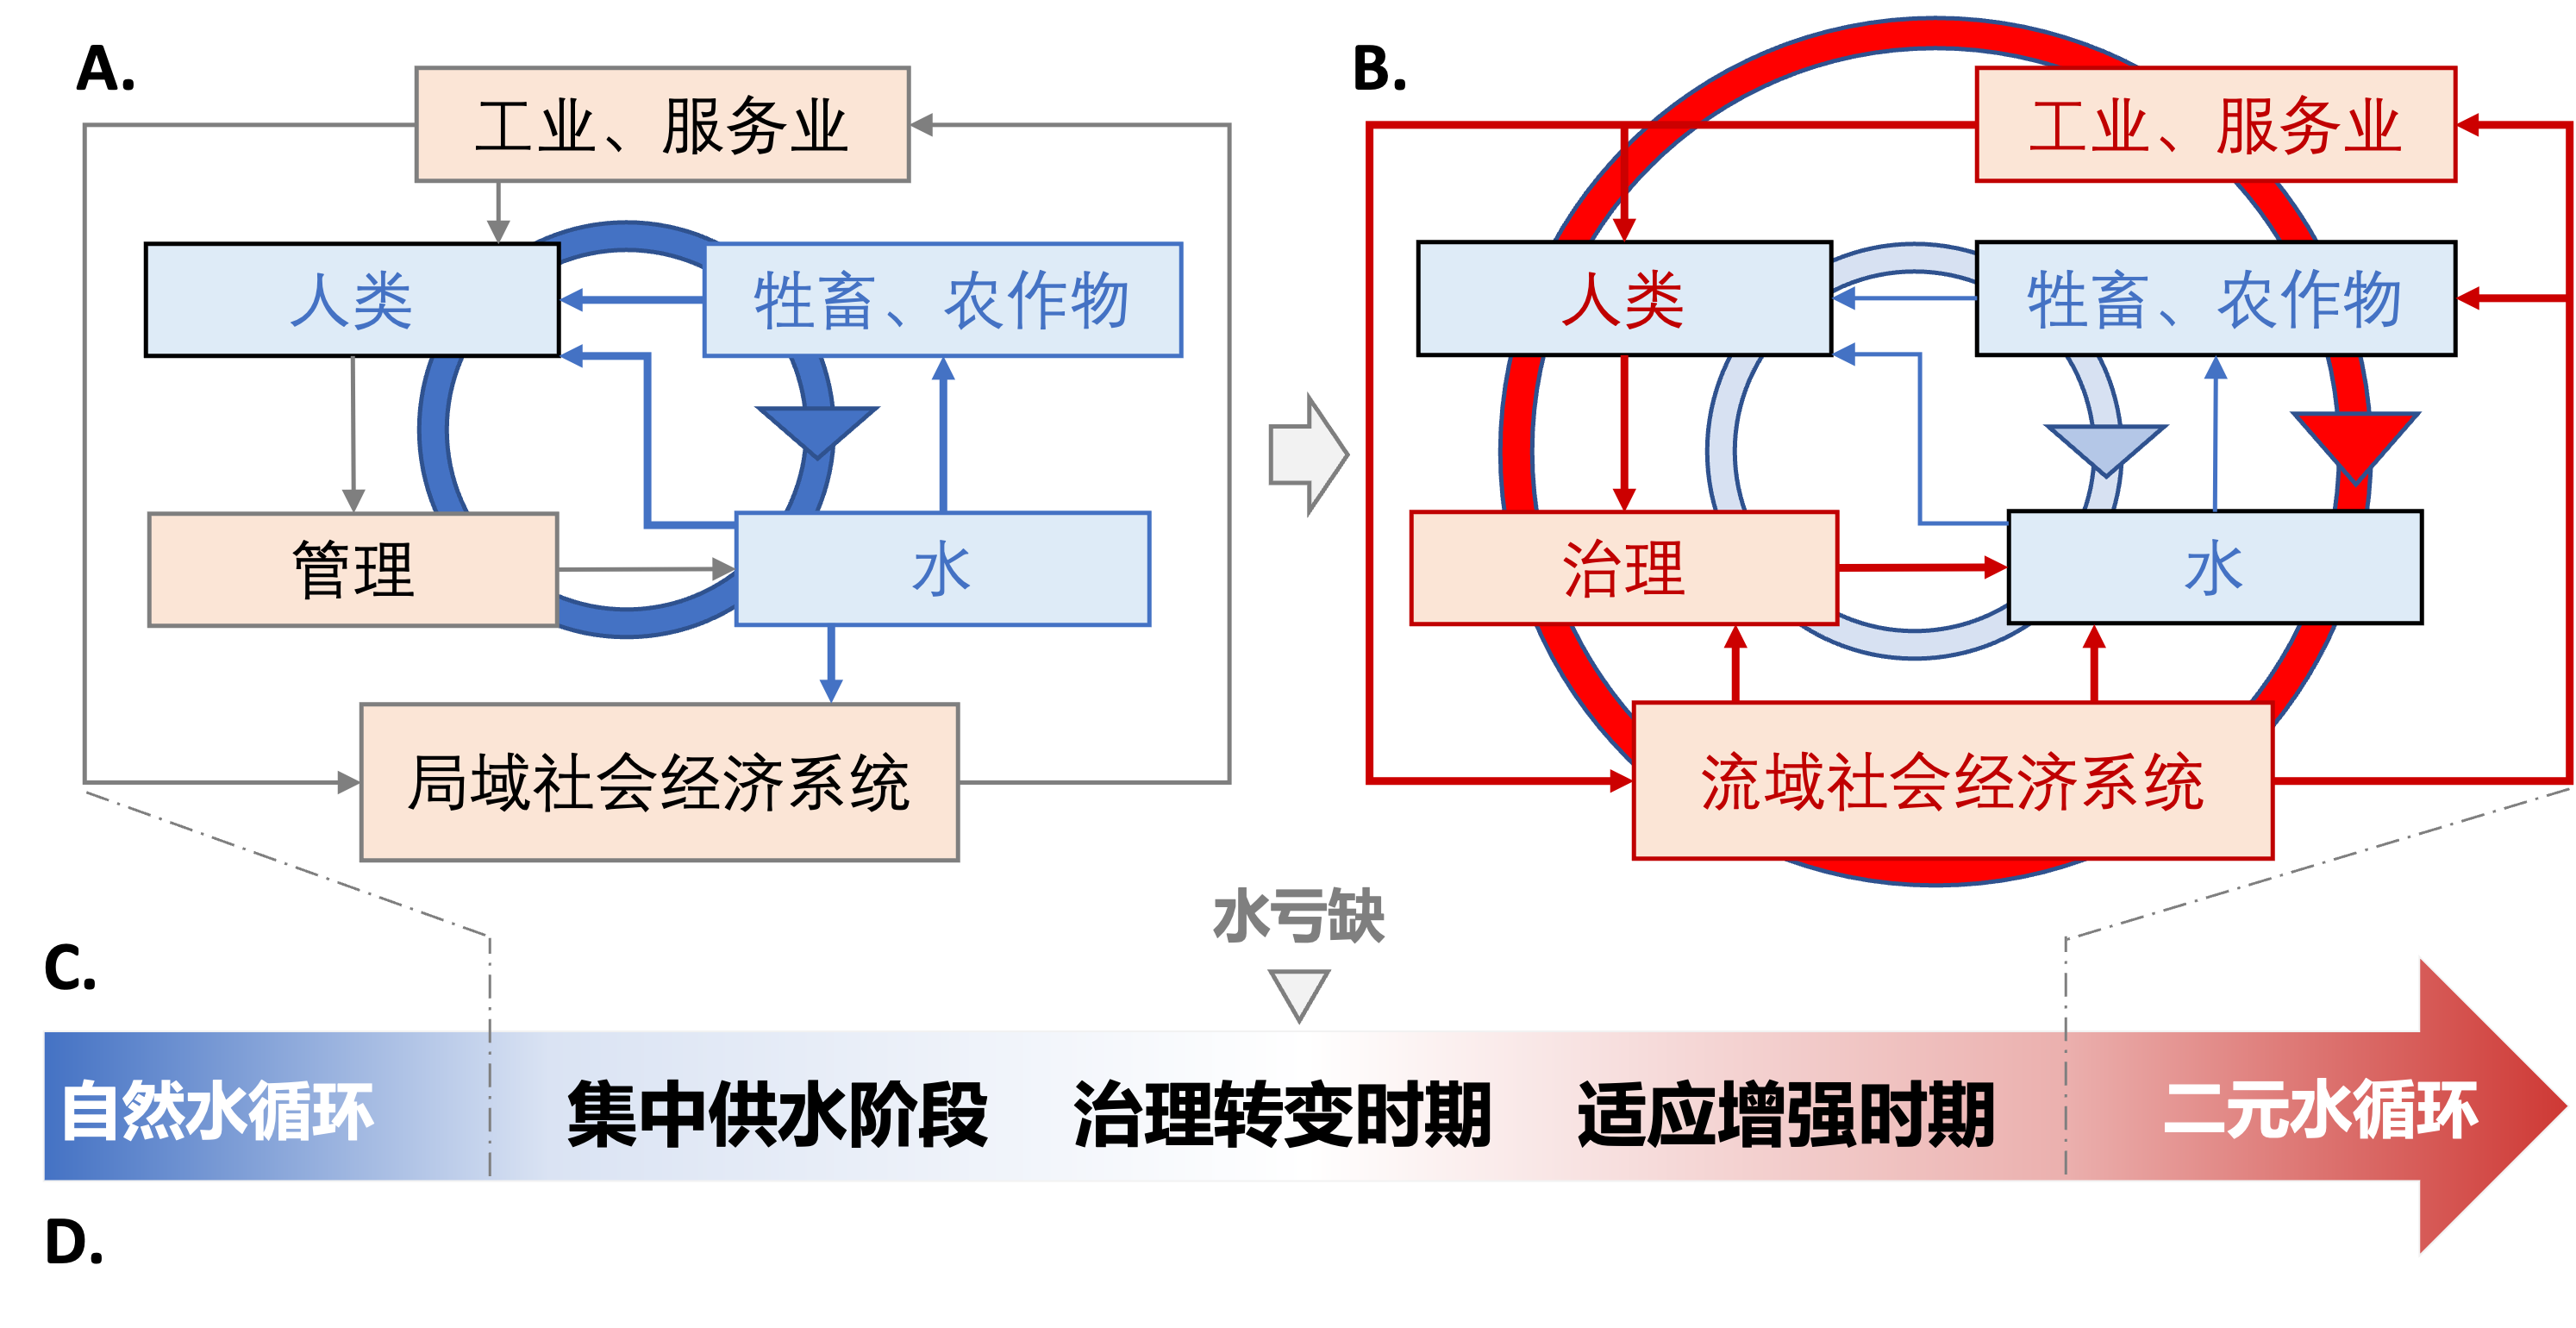
\includegraphics[width=\textwidth]{img/ch4/ch4_transition.png}
	\caption[人类主导下流域系统的水治理阶段过渡]{
		人类主导下流域系统的水治理变化过程。蓝色代表人类活动尚未成为主导的社会-水文循环,红色代表由社会经济过程主导的流域水过程。
        \textbf{A.}随着社会经济系统的发展,用以非供给服务的水需求增加;同时,通过水库等工程措施使人们能够控制水循环并局部缓解水资源压力。
        \textbf{B.}随着人为干预升级,不同地区和部门间的用水权衡愈发突出;流域亟需提升利用效率和调度能力,并组织起的更具适应性的水治理。
        \textbf{C.}在人类主导的流域社会-水文循环模式下,水治理转变常发生在水资源亏缺之后,在社会-经济过程主导下推动适应能力快速增长。在此之前水治理主要面临经济和环境挑战,但随后面临社会和政策挑战。
	}\label{fig:summary}
\end{figure}

\section{对流域治理规律的启示}

通过在数据丰富的黄河流域进行应用,本章研究表明所有的水治理问题都会导致“谁获得水、何时获得水以及如何获得水”的改变,因此监测“有多少水、怎么用、怎么分”三个关键问题对识别流域水治理变化有极大帮助。
但在世界范围内广泛应用该方法的主要局限是缺乏全球尺度的长时间序列数据,这意味着IWGI的可能缺点是难以推广。
在数据相对不足的流域应用IWGI时,建议不同方面的指标选择可根据现有数据集进行调整,因为底层指标之间关系的变化趋势比精确计算指标更重要。
在当今这个“人类世”,人-水关系由人类活动所主导的情况越来越普遍,应对层出不穷的治理挑战已成为复杂的人-水系统的核心\cite{cumming2018,cumming2014,jaeger2019}。
许多流域仍在不断接近系统随时可能崩溃的“地球界限”\cite{gleeson2020, wang-erlandsson2022},只有更深入地理解流域水治理系统,结合非线性稳态变化和转型的思想,才能维持流域社会-生态系统的韧性并实现可持续、高质量发展\cite{falkenmark2019}。

% Implications
由于大型河流流域是生态系统服务、经济发展和人类福祉的关键来源,水治理逐渐从主要的地方问题成为国家或国际问题\cite{best2019,best2020}。
随着远程耦合在联系日益紧密的世界中提出了更多的水治理挑战,水治理的政权转变与不同的人与水的关系相一致\cite{diaz2019}。
这一过程反映了社会如何通过增强其在水社会循环中的适应能力来改变治理实践的建议,IWGI定量地确定了这一转变\cite{loch2020,turton1999}。
科学家和决策者认识到不断变化的治理挑战是至关重要的,因为在一个阶段下开发的模型、制度、工程和方法不一定适用于另一个治理阶段\cite{reyers2018}。


\section{小结}\label{ch4:summary}
% 本章整合了水文数据、统计数据、历史文献材料等多源数据,开发流域水治理综合指数(Integrated Water Governance Index, IWGI),利用突变点检测方法量化识别了二十世纪六十年代以来的黄河流域治理的阶段变化,并分析了转变发生的驱动因素。

本章研究表明,两个突变点可以将1965 - 2013 年的黄河流域水治理演变历史划分为明显的三个阶段,依据其各自特点可命名为:集中供水时期(1965 - 1978,P1)、治理转变时期(1979 - 2001,P2)、适应增强时期(2002 - 2013,P3),而“稀缺情况(S)”、“使用目的(P)”和“分配方式(A)”的三个方面的指标在各阶段为黄河流域水治理的特征变化做出了不同贡献。
进一步探讨致使IWGI变化的原因,灌溉区扩张及工业和服务业的经济增长是推动“集中供水时期”和“治理转变时期”两个阶段变化的主要原因,环境背景、社会文化等因素对不同阶段的指标变化都产生了影响,水治理政策是将“治理转变时期”推向“适应增强时期”的主要驱动力。

黄河流域的水治理演化过程是“增大供给、治理转变、适应增强”的突出的案例,而其变化规律已在全球由人类主导的流域社会-水文循环过程中广泛出现。
理解黄河流域水治理的变化规律,可以为快速变化的大河流域提供实现可持续性的重要理论依据。

% Implications
由于大型河流流域是生态系统服务、经济发展和人类福祉的关键来源,水治理逐渐从主要的地方问题成为国家或国际问题\cite{best2019,best2020}。
随着远程耦合在联系日益紧密的世界中提出了更多的水治理挑战,水治理的政权转变与不同的人与水的关系相一致\cite{diaz2019}。
这一过程反映了社会如何通过增强其在水社会循环中的适应能力来改变治理实践的建议,IWGI定量地确定了这一转变\cite{loch2020,turton1999}。
科学家和决策者认识到不断变化的治理挑战是至关重要的,因为在一个阶段下开发的模型、制度、工程和方法不一定适用于另一个治理阶段\cite{reyers2018}。

\label{chapter4}

%%% 其它部分
%\backmatter

% 
 % 参考文献
 \bibliographystyle{bnubib}
 \bibliography{ref/refs}

% 附录
%\begin{appendix}
%% !Mode:: "TeX:UTF-8"
%%% Local Variables: 
%%% mode: latex
%%% TeX-master: "../main"
%%% End: 

\chapter{外文资料原文}
\label{cha:engorg}
As one of the most widely used techniques in operations research, {\em
  mathematical programming} is defined as a means of maximizing a quantity known
as {\em objective function}, subject to a set of constraints represented by
equations and inequalities. Some known subtopics of mathematical programming are
linear programming, nonlinear programming, multiobjective programming, goal
programming, dynamic programming, and multilevel programming$^{[1]}$.

It is impossible to cover in a single chapter every concept of mathematical
programming. This chapter introduces only the basic concepts and techniques of
mathematical programming such that readers gain an understanding of them
throughout the book$^{[2,3]}$.


\section{Single-Objective Programming}
The general form of single-objective programming (SOP) is written
as follows,
\begin{equation}\tag*{(123)} % 如果附录中的公式不想让它出现在公式索引中,那就请
                             % 用 \tag*{xxxx}
\left\{\begin{array}{l}
\max \,\,f(x)\\[0.1 cm]
\mbox{subject to:} \\ [0.1 cm]
\qquad g_j(x)\le 0,\quad j=1,2,\cdots,p
\end{array}\right.
\end{equation}
which maximizes a real-valued function $f$ of
$x=(x_1,x_2,\cdots,x_n)$ subject to a set of constraints.

\newtheorem{mpdef}{Definition}[chapter]
\begin{mpdef}
In SOP, we call $x$ a decision vector, and
$x_1,x_2,\cdots,x_n$ decision variables. The function
$f$ is called the objective function. The set
\begin{equation}\tag*{(456)} % 这里同理,其它不再一一指定。
S=\left\{x\in\Re^n\bigm|g_j(x)\le 0,\,j=1,2,\cdots,p\right\}
\end{equation}
is called the feasible set. An element $x$ in $S$ is called a
feasible solution.
\end{mpdef}

\newtheorem{mpdefop}[mpdef]{Definition}
\begin{mpdefop}
A feasible solution $x^*$ is called the optimal
solution of SOP if and only if
\begin{equation}
f(x^*)\ge f(x)
\end{equation}
for any feasible solution $x$.
\end{mpdefop}

One of the outstanding contributions to mathematical programming was known as
the Kuhn-Tucker conditions\ref{eq:ktc}. In order to introduce them, let us give
some definitions. An inequality constraint $g_j(x)\le 0$ is said to be active at
a point $x^*$ if $g_j(x^*)=0$. A point $x^*$ satisfying $g_j(x^*)\le 0$ is said
to be regular if the gradient vectors $\nabla g_j(x)$ of all active constraints
are linearly independent.

Let $x^*$ be a regular point of the constraints of SOP and assume that all the
functions $f(x)$ and $g_j(x),j=1,2,\cdots,p$ are differentiable. If $x^*$ is a
local optimal solution, then there exist Lagrange multipliers
$\lambda_j,j=1,2,\cdots,p$ such that the following Kuhn-Tucker conditions hold,
\begin{equation}
\label{eq:ktc}
\left\{\begin{array}{l}
    \nabla f(x^*)-\sum\limits_{j=1}^p\lambda_j\nabla g_j(x^*)=0\\[0.3cm]
    \lambda_jg_j(x^*)=0,\quad j=1,2,\cdots,p\\[0.2cm]
    \lambda_j\ge 0,\quad j=1,2,\cdots,p.
\end{array}\right.
\end{equation}
If all the functions $f(x)$ and $g_j(x),j=1,2,\cdots,p$ are convex and
differentiable, and the point $x^*$ satisfies the Kuhn-Tucker conditions
(\ref{eq:ktc}), then it has been proved that the point $x^*$ is a global optimal
solution of SOP.

\subsection{Linear Programming} 
\label{sec:lp}

If the functions $f(x),g_j(x),j=1,2,\cdots,p$ are all linear, then SOP is called
a {\em linear programming}.

The feasible set of linear is always convex. A point $x$ is called an extreme
point of convex set $S$ if $x\in S$ and $x$ cannot be expressed as a convex
combination of two points in $S$. It has been shown that the optimal solution to
linear programming corresponds to an extreme point of its feasible set provided
that the feasible set $S$ is bounded. This fact is the basis of the {\em simplex
  algorithm} which was developed by Dantzig as a very efficient method for
solving linear programming.
\begin{table}[ht]
\centering
  \centering
  \caption*{Table~1\hskip1em This is an example for manually numbered table, which would not appear in the list of tables}
  \label{tab:badtabular2}
  \begin{tabular}[c]{|c|m{0.8in}|c|c|c|c|c|}\hline
    \multicolumn{2}{|c|}{Network Topology} & \# of nodes & 
    \multicolumn{3}{c|}{\# of clients} & Server \\\hline
    GT-ITM & Waxman Transit-Stub & 600 &
    \multirow{2}{2em}{2\%}& 
    \multirow{2}{2em}{10\%}& 
    \multirow{2}{2em}{50\%}& 
    \multirow{2}{1.2in}{Max. Connectivity}\\\cline{1-3}
    \multicolumn{2}{|c|}{Inet-2.1} & 6000 & & & &\\\hline
    \multirow{2}{1in}{Xue} & Rui  & Ni &\multicolumn{4}{c|}{\multirow{2}*{\bnuthesis}}\\\cline{2-3}
    & \multicolumn{2}{c|}{ABCDEF} &\multicolumn{4}{c|}{} \\\hline
\end{tabular}  
\end{table}

Roughly speaking, the simplex algorithm examines only the extreme points of the
feasible set, rather than all feasible points. At first, the simplex algorithm
selects an extreme point as the initial point. The successive extreme point is
selected so as to improve the objective function value. The procedure is
repeated until no improvement in objective function value can be made. The last
extreme point is the optimal solution.

\subsection{Nonlinear Programming}

If at least one of the functions $f(x),g_j(x),j=1,2,\cdots,p$ is nonlinear, then
SOP is called a {\em nonlinear programming}.

A large number of classical optimization methods have been developed to treat
special-structural nonlinear programming based on the mathematical theory
concerned with analyzing the structure of problems.

Now we consider a nonlinear programming which is confronted solely with
maximizing a real-valued function with domain $\Re^n$.  Whether derivatives are
available or not, the usual strategy is first to select a point in $\Re^n$ which
is thought to be the most likely place where the maximum exists. If there is no
information available on which to base such a selection, a point is chosen at
random. From this first point an attempt is made to construct a sequence of
points, each of which yields an improved objective function value over its
predecessor. The next point to be added to the sequence is chosen by analyzing
the behavior of the function at the previous points. This construction continues
until some termination criterion is met. Methods based upon this strategy are
called {\em ascent methods}, which can be classified as {\em direct methods},
{\em gradient methods}, and {\em Hessian methods} according to the information
about the behavior of objective function $f$. Direct methods require only that
the function can be evaluated at each point. Gradient methods require the
evaluation of first derivatives of $f$. Hessian methods require the evaluation
of second derivatives. In fact, there is no superior method for all
problems. The efficiency of a method is very much dependent upon the objective
function.


\chapter{外文资料的调研阅读报告或书面翻译}
\section{单目标规划}
北冥有鱼,其名为鲲。鲲之大,不知其几千里也。化而为鸟,其名为鹏。鹏之背,不知其几
千里也。怒而飞,其翼若垂天之云。是鸟也,海运则将徙于南冥。南冥者,天池也。 
\begin{equation}\tag*{(123)}
 p(y|\mathbf{x}) = \frac{p(\mathbf{x},y)}{p(\mathbf{x})}=
\frac{p(\mathbf{x}|y)p(y)}{p(\mathbf{x})}
\end{equation}

吾生也有涯,而知也无涯。以有涯随无涯,殆已!已而为知者,殆而已矣!为善无近名,为
恶无近刑,缘督以为经,可以保身,可以全生,可以养亲,可以尽年。

\subsection{线性规划}
庖丁为文惠君解牛,手之所触,肩之所倚,足之所履,膝之所倚,砉然响然,奏刀騞然,莫
不中音,合于桑林之舞,乃中经首之会。
\begin{table}[ht]
\centering
  \caption*{表~A1\hskip1em 这是手动编号但不出现在索引中的一个表格例子}
  \label{tab:badtabular3}
  \begin{tabular}[c]{|c|m{0.8in}|c|c|c|c|c|}\hline
    \multicolumn{2}{|c|}{Network Topology} & \# of nodes & 
    \multicolumn{3}{c|}{\# of clients} & Server \\\hline
    GT-ITM & Waxman Transit-Stub & 600 &
    \multirow{2}{2em}{2\%}& 
    \multirow{2}{2em}{10\%}& 
    \multirow{2}{2em}{50\%}& 
    \multirow{2}{1.2in}{Max. Connectivity}\\\cline{1-3}
    \multicolumn{2}{|c|}{Inet-2.1} & 6000 & & & &\\\hline
    \multirow{2}{1in}{Xue} & Rui  & Ni &\multicolumn{4}{c|}{\multirow{2}*{\bnuthesis}}\\\cline{2-3}
    & \multicolumn{2}{c|}{ABCDEF} &\multicolumn{4}{c|}{} \\\hline
\end{tabular}  
\end{table}

\begin{table}[ht]
\centering
  \caption{正常附录表格的例子}
  \label{tab:badtabular3}
  \begin{tabular}[c]{|c|m{0.8in}|c|c|c|c|c|}\hline
    \multicolumn{2}{|c|}{Network Topology} & \# of nodes & 
    \multicolumn{3}{c|}{\# of clients} & Server \\\hline
    GT-ITM & Waxman Transit-Stub & 600 &
    \multirow{2}{2em}{2\%}& 
    \multirow{2}{2em}{10\%}& 
    \multirow{2}{2em}{50\%}& 
    \multirow{2}{1.2in}{Max. Connectivity}\\\cline{1-3}
    \multicolumn{2}{|c|}{Inet-2.1} & 6000 & & & &\\\hline
    \multirow{2}{1in}{Xue} & Rui  & Ni &\multicolumn{4}{c|}{\multirow{2}*{\bnuthesis}}\\\cline{2-3}
    & \multicolumn{2}{c|}{ABCDEF} &\multicolumn{4}{c|}{} \\\hline
\end{tabular}  
\end{table}

文惠君曰:“嘻,善哉!技盖至此乎?”庖丁释刀对曰:“臣之所好者道也,进乎技矣。始臣之
解牛之时,所见无非全牛者;三年之后,未尝见全牛也;方今之时,臣以神遇而不以目视,
官知止而神欲行。依乎天理,批大郤,导大窾,因其固然。技经肯綮之未尝,而况大坬乎!
良庖岁更刀,割也;族庖月更刀,折也;今臣之刀十九年矣,所解数千牛矣,而刀刃若新发
于硎。彼节者有间而刀刃者无厚,以无厚入有间,恢恢乎其于游刃必有余地矣。是以十九年
而刀刃若新发于硎。虽然,每至于族,吾见其难为,怵然为戒,视为止,行为迟,动刀甚微,
謋然已解,如土委地。提刀而立,为之而四顾,为之踌躇满志,善刀而藏之。”

文惠君曰:“善哉!吾闻庖丁之言,得养生焉。”


\subsection{非线性规划}
孔子与柳下季为友,柳下季之弟名曰盗跖。盗跖从卒九千人,横行天下,侵暴诸侯。穴室枢
户,驱人牛马,取人妇女。贪得忘亲,不顾父母兄弟,不祭先祖。所过之邑,大国守城,小
国入保,万民苦之。孔子谓柳下季曰:“夫为人父者,必能诏其子;为人兄者,必能教其弟。
若父不能诏其子,兄不能教其弟,则无贵父子兄弟之亲矣。今先生,世之才士也,弟为盗
跖,为天下害,而弗能教也,丘窃为先生羞之。丘请为先生往说之。”

柳下季曰:“先生言为人父者必能诏其子,为人兄者必能教其弟,若子不听父之诏,弟不受
兄之教,虽今先生之辩,将奈之何哉?且跖之为人也,心如涌泉,意如飘风,强足以距敌,
辩足以饰非。顺其心则喜,逆其心则怒,易辱人以言。先生必无往。”

孔子不听,颜回为驭,子贡为右,往见盗跖。


\chapter{其它附录}
前面两个附录主要是给本科生做例子。其它附录的内容可以放到这里,当然如果你愿意,可
以把这部分也放到独立的文件中,然后将其 \verb|\input| 到主文件中。
%\end{appendix}
% 
% % 学术成果
% !Mode:: "TeX:UTF-8"
% chktex-file 8

\begin{paper}
\begin{enumerate}
	\item \textbf{Song, S.}, Wang, S., Wu, X., Huang, Y. \& Fu, B. Decreased virtual water outflows from the Yellow River basin are increasingly critical to China. Hydrology and Earth System Sciences 26, 2035-2044 (2022). % (IF = 6.62) 
	\item \textbf{Song, S.} et al. Sediment transport under increasing anthropogenic stress: Regime shifts within the Yellow River, China. Ambio 49, 2015-2025 (2020). % (IF = 6.94) 
	\item \textbf{Song, S.} et al. Improving representation of collective memory in socio-hydrological models and new insights into flood risk management. J Flood Risk Management 14, (2021). % (IF = 4.01) 
	\item \textbf{Song, S.} et al. The responses of Spinifex littoreus to sand burial on the coastal area of Pingtan Island, Fujian Province, South China. Écoscience 1-10 (2021). % (IF = 1.34) 
	\item Wang, S., \textbf{Song, S.}, Zhang, J., Wu, X. \& Fu, B. Achieving a fit between social and ecological systems in drylands for sustainability. Curr. Opin. Environ. Sustain. 48, 53-58 (2021). % (IF = 7.96) 
	\item \textbf{宋爽}, 王帅, 傅伯杰, 陈海滨, 刘焱序, 赵文武. 社会—生态系统适应性治理研究进展与展望. 地理学报, 74, 2401-2410 (2019). % (IF = 10.14) 
	% 接下来是合著
	\item Wu, X., Fu, B. J., Wang S., \textbf{Song S.}, et al. Decoupling of SDGs followed by re-coupling as sustainable development progresses. Nature Sustainability (2022) doi:10.1038/s41893- 022-00868-x. % (IF = 27.2)
	\item Jiao, C., Wang, S., \textbf{Song, S.}, Fu B., Long-term and Seasonal Variation of Open-surface Water Bodies in the Yellow River Basin during 1990-2020. Hydrological Processes, e14846 (2023).
	\item Chen, P., Wang, S., \textbf{Song, S.}, Wang Y., Wang Y., Gao D., Li Z. Ecological restoration intensifies evapotranspiration in the Kubuqi Desert. Ecological Engineering 175, 106504 (2022). % (IF = 4.37) 
	\item Yao, Y., Fu, B., Liu, Y., Wang, Y., \& \textbf{Song, S.} The contribution of ecosystem restoration to sustainable development goals in Asian drylands: A literature review. Land Degrad Dev ldr.4065 (2021). % (IF = 4.38)
	\item Zhang, M., Wang S., Fu, B.J., Wei, X. H., Wang, C., \textbf{Song, S.} Structure Disentanglement and Effect Analysis of the Arid Riverscape Social-Ecological System Using a Network Approach. Sustainability 11, 5159 (2019). % (IF = 3.89) 
	\item Gao, D. Wang, S. Li, Z.D., Wei. F. L., Chen, P., \textbf{Song, S.}. Threshold of vapour- pressure deficit constraint on light use efficiency varied with soil water content. Ecohydrology (2021) doi:10.1002/eco.2305. % (IF = 3.17) 
	\item Li, Z., Wang, S., \textbf{Song, S.}, Wang, Y. \& Musakwa, W. Detecting land degradation in Southern Africa using Time Series Segment and Residual Trend (TSS-RESTREND). Journal of Arid Environments 184, 104314 (2021). % (IF = 2.76) 
	\item 王奕佳, 刘焱序, \textbf{宋爽}, 姚莹, 傅伯杰. 社区尺度社会\textendash{}生态系统适应途径述评. 地理科学进展, 41, 935-944 (2022). % (IF = 6.05) 
	\item 王奕佳, 刘焱序, \textbf{宋爽}, 傅伯杰. 水—粮食—能源—生态系统关联研究进展. 地球科学进展, 36, 684-693 (2021). % (IF = 6.04) 
	
	% \item Yang Y, Ren T L, Zhang L T, et al. Miniature microphone with silicon-based ferroelectric thin films. Integrated Ferroelectrics, 2003, 52:229-235. (SCI 收录, 检索号:758FZ.)
	% \item 杨轶, 张宁欣, 任天令, 等. 硅基铁电微声学器件中薄膜残余应力的研究. 中国机械工程, 2005, 16(14):1289-1291. (EI 收录, 检索号:0534931 2907.)
	% \item 杨轶, 张宁欣, 任天令, 等. 集成铁电器件中的关键工艺研究. 仪器仪表学报,2003, 24(S4):192-193. (EI 源刊.)
	% \item Yang Y, Ren T L, Zhu Y P, et al. PMUTs for handwriting recognition. Inpress. (已被 Integrated Ferroelectrics 录用. SCI 源刊.)
	% \item Wu X M, Yang Y, Cai J, et al. Measurements of ferroelectric MEMS microphones. Integrated Ferroelectrics, 2005, 69:417-429. (SCI 收录, 检索号:896KM.)
	% \item 贾泽, 杨轶, 陈兢, 等. 用于压电和电容微麦克风的体硅腐蚀相关研究. 压电与声光, 2006, 28(1):117-119. (EI 收录, 检索号:06129773469.)
	% \item 伍晓明, 杨轶, 张宁欣, 等. 基于MEMS技术的集成铁电硅微麦克风. 中国集成电路, 2003, 53:59-61.
\end{enumerate}
\end{paper}


% 致谢
% !Mode:: "TeX:UTF-8"


\begin{ack}

    转眼间,我研究了五年的人与河。河有四时,有盈亏,有荣枯,亦有喜乐哀愁。河没有名字,我在河中打着水漂,所有想说的话河便替我说了——

    人顺河而下,可期百川入海。
    
    感谢恩师傅伯杰院士,学研若沧茫大海,取扁舟一叶横渡,他是“大渡海”的引路人。傅老师的教诲总是简单直接又具有启发性,帮助我这位五年前还徘徊在海边「面朝西边,指向北方」的少年找到了渡海的起点。感谢王帅教授,他包容着我的自由随性,倾听我的理想主义,给我开卷阅读的空间,给我自主探索的时间。渡海途中,我不止一次想对他说「Oh, captain, my captain」!
    
    感谢武旭同老师,从五年前野外相识起,他见证并影响着我的学术思想之演变,几乎每一篇研究工作我都曾向他请教,并总是能得到极有价值的建议。还要感谢北京师范大学许多优秀的老师们,包括但不限于赵文武老师、刘焱序老师、李琰老师、周沙老师、沈妙根老师、缪驰远老师,感谢你们曾在不同场合对我的研究工作做出的指点和帮助。感谢中山大学一直同我保持联系的杜建会老师和胡亮老师,杜老师的敢想敢做与亮哥的认真严谨,都是我学术路途中后知后觉的宝贵财富。
    
    人沿河而行,可辨成长足迹。
    
    感谢可爱的品言,她是不断让我清醒地认识到“人生不止有一个奖章”的灵魂伴侣,她淬炼我的天真与敏锐,使我的好奇心与求知欲常驻。感谢我博士期间的两位舍友卢文路与骆玉川,与他们同处的日常绝不会有一丝枯燥无趣。感谢王奕佳师妹,从中山大学到北师大,从青藏高原到维也纳,她永远是最值得信赖的的战友。感谢其他同院的挚友们,陈鹏、宋佳熙、张疋亥、冯思远,在学术和生活中他们都是能与之畅所欲言的伙伴。感谢课题组各位同仁,尤其是王亚萍、张皓宇、焦晨泰、叶冲冲、高德新、谭子敏,他们在举不胜举的琐事上提供的帮助与支持,使科研生活的点滴得以汇聚成流。
    
    感谢香港大学的李研师兄,五年来他恰到好处的点拨让本不会编程的我逐步将短板补长。感谢北京大学的王文宇与黄永源,中国人民大学的牛昱尧、张炼、与温慧瑜,同他们在经济、历史、考古、社会学等领域的定期探讨极大地开拓了我的视野。感谢我的桥牌搭档、北京大学的肖逸南,他在许多数学问题上给予了我莫大帮助,对我而言好似数次雪中送炭。感谢所有为我提供过资料、信息、修改意见的老师同学乃至陌生审稿人们,我想对你们付出的答谢已毋需言表——我从来没有忽视过任何有价值的建议。
    
    人溯河回望,可见源头活水。
    
    感谢我的父母,他们一直努力为我营造着独立自主、无忧无虑的学习环境。他们默默操持着我们的家,即便来探望我,也会说着「我们看过北京了,我们看过珠海了,我们回家吧」之类的话,只因不想从学业中分走我太多精力。文章我自甘沦落,不觅封侯但觅诗,也许我永远无法成为一个世俗意义上的成功者,但多亏他们的支持,我才能在自己喜欢的道路上坚定前行,我走过的每一段路,笔下的每一个字符,都饱含他们的理解与厚爱。
    
    感谢互联网世界为我提供过帮助的众多开源社区和开源工具,你们使我能够自由勾勒出脑海里的玉宇琼楼,而不必从「先造一颗轮子」开始。功不唐捐无须先磨细铁杵,我心中本有的针才不会荒芜。工具的快速迭代也督促着我保持终身学习,哪怕世上的一切终将腐朽,拥抱开源的人也不必在一天内吃掉五十罐凤梨罐头。
    
    最后,致敬我的精神导师们——爱德华·威尔逊,段义孚,大卫·爱登堡,你们的作品是指引我前进的光,去追寻那个人与自然和谐共处的世界。你们用一份了不起的优雅,维持住了那个世界的幻觉,尽管那里的一切要么未曾到来,要么已经逝去\ldots
    
    悠悠五载换拙文百页,忽忽万绪聚笔尖一言。读博乃极尽自私之事,沿途固多承善意,然答报时光益疏,纵有穷尽感恩之思,终渺沧海之一粟。未尽之人事,今朝情谊铭心坊,来日重逢待报梅。
\end{ack}


\end{document}
